\documentclass[a4paper, oneside, 11pt]{book}

\textwidth 145mm
\topmargin -2mm
\textheight 235mm

\usepackage[czech]{babel}
\usepackage[utf8]{inputenc}
\usepackage[T1]{fontenc}
\usepackage{amsmath}
\usepackage{amsfonts}
\usepackage{amssymb}
\usepackage{graphicx}
\usepackage{fancyhdr}
\usepackage[]{quotchap}
\usepackage{mdwlist}
\usepackage{verbatim}




% nastaveni zahlavi
\pagestyle{fancy}
\fancyfoot{}
\fancyfoot[L]{} 
\fancyfoot[R]{} 
\fancyfoot[C]{\thepage}
\renewcommand{\headrulewidth}{0.4pt} 
\fancyhead{}
\fancyhead[RO]{\rightmark}
\fancyhead[LE]{\leftmark}

% nastaveni nazvu kapitoly
\renewcommand\chapterheadstartvskip{\vspace*{-4\baselineskip}}

% nastaveni tučného bezpatkového písma
\DeclareMathAlphabet{\mathsfb}{T1}{lcmss}{b}{sl}

\newcommand{\me}{\mathrm{e\,}} % Eulerovo cislo
\newcommand{\mi}{\mathrm{i}} % komplexni jednotka
\newcommand{\mj}{\mathrm{j}} % komplexni jednotka
\newcommand{\dif}{\,\mathrm{d}} % diferencial
\newcommand{\mat}[1]{\mathrm{\mathbf{{#1}}}} % tenzor nebo matice
\renewcommand{\vec}[1]{\mbox{\boldmath$#1$}} % vektor
\newcommand{\faz}[1]{{\underline{#1}}} % fazor
\newcommand{\vecfaz}[1]{\mbox{\underline{\boldmath$#1$}}} % fazor vektoru
\newcommand*{\unit}[1]{\ensuremath{\mathrm{\ #1}}} % jednotky
\newcommand{\degree}{\ensuremath{^{\circ}\mathrm{C}}} % stupne Celsia
\renewcommand{\Re}{\mathrm{Re}} % imaginarni cast
\renewcommand{\Im}{\mathrm{Im}} % realna cast
\newcommand{\tg}{\mathrm{tg}\ } % tangens
\newcommand{\grad}{\mathrm{grad}\ } % gradient
\newcommand{\curl}{\mathrm{curl}\ } % rotace
\newcommand{\rot}{\mathrm{rot}\ } % rotace
\renewcommand{\div}{\mathrm{div}\ } % divergence
\newcommand{\const}{\mathrm{const}} % konstanta
\newcommand{\konst}{\mathrm{konst}} % konstanta

% nastaveni vysky bunek tabulek
\renewcommand\arraystretch{1.2}

\makeatletter
\g@addto@macro\@verbatim\footnotesize
\makeatother 

% nastavení dělení/nedělení slov
% \hyphenation{de-finovaném}
\hyphenation{ele-ktro-mag-ne-ti-cké}

\begin{document}
%% !TeX root = Main.tex

\begin{titlepage}
\begin{center}

\noindent {\Large \textbf{Katedra aplikované elektroniky a telekomunikací}} \\
\vspace*{0.3cm}
\noindent {\Large \textbf{Fakulta elektrotechnická}} \\
\vspace*{0.5cm}
\noindent {\Large \textbf{Západočeská univerzita v~Plzni}} \\
\vspace*{9cm}
%\noindent {\LARGE \textsc{Diplomová práce}} \\
\noindent {\LARGE \textbf{DIPLOMOVÁ PRÁCE}} \\
\vspace*{11cm}
\noindent {\Large \textbf{2011}} \hspace{8cm} {\Large\textsc{Bc. Lukáš Koudela}} \\
\end{center}
\end{titlepage}
\titlepage
%% !TeX root = Main.tex

\begin{titlepage}
\begin{center}

\noindent {\Large \textbf{Západočeská univerzita v~Plzni}} \\
\vspace*{0.5cm}
\noindent {\Large \textbf{Fakulta elektrotechnická}} \\
\vspace*{0.5cm}
\noindent {\Large \textbf{Katedra elektromechaniky a výkonové elektroniky}} \\
\vspace*{4cm}
\noindent {\Large \textsc{Lukáš Koudela}} \\
\vspace*{3cm}
\noindent {\huge \textbf{SIMULACE ŠÍŘENÍ ELEKTROMAGNETICKÝCH VLN}} \\
\vspace*{3cm}
%\noindent {\LARGE \textsc{Diplomová práce}} \\
\noindent {\LARGE \textbf{DIPLOMOVÁ PRÁCE}} \\
\vspace*{8cm}
\noindent {\Large \textbf{2011}} \\
\end{center}
\end{titlepage}
\titlepage
%% !TeX root = Main.tex

\renewcommand\thepage{}
\begin{figure}[!h]
	\centering
	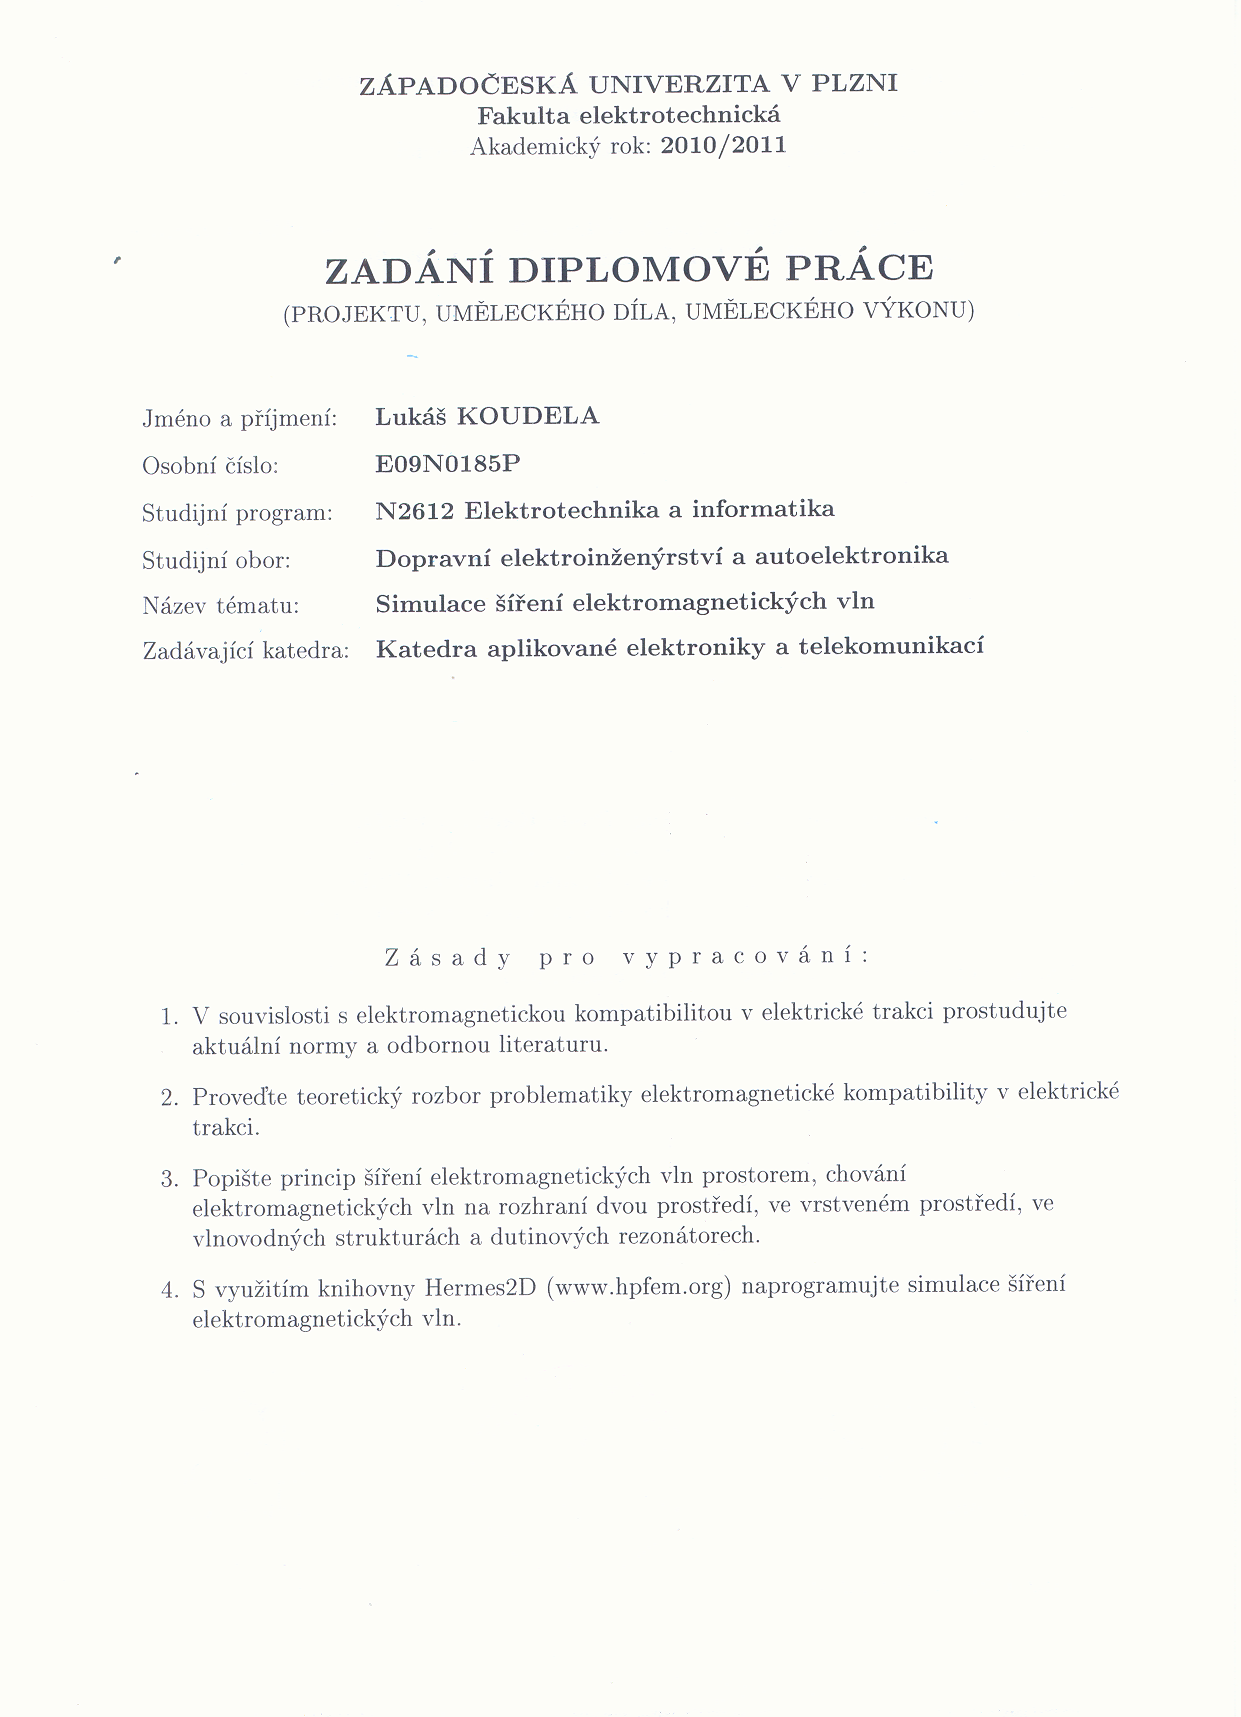
\includegraphics[width=15cm]{zadani1.png}
\end{figure}
\titlepage
\begin{figure}[!h]
	\centering
	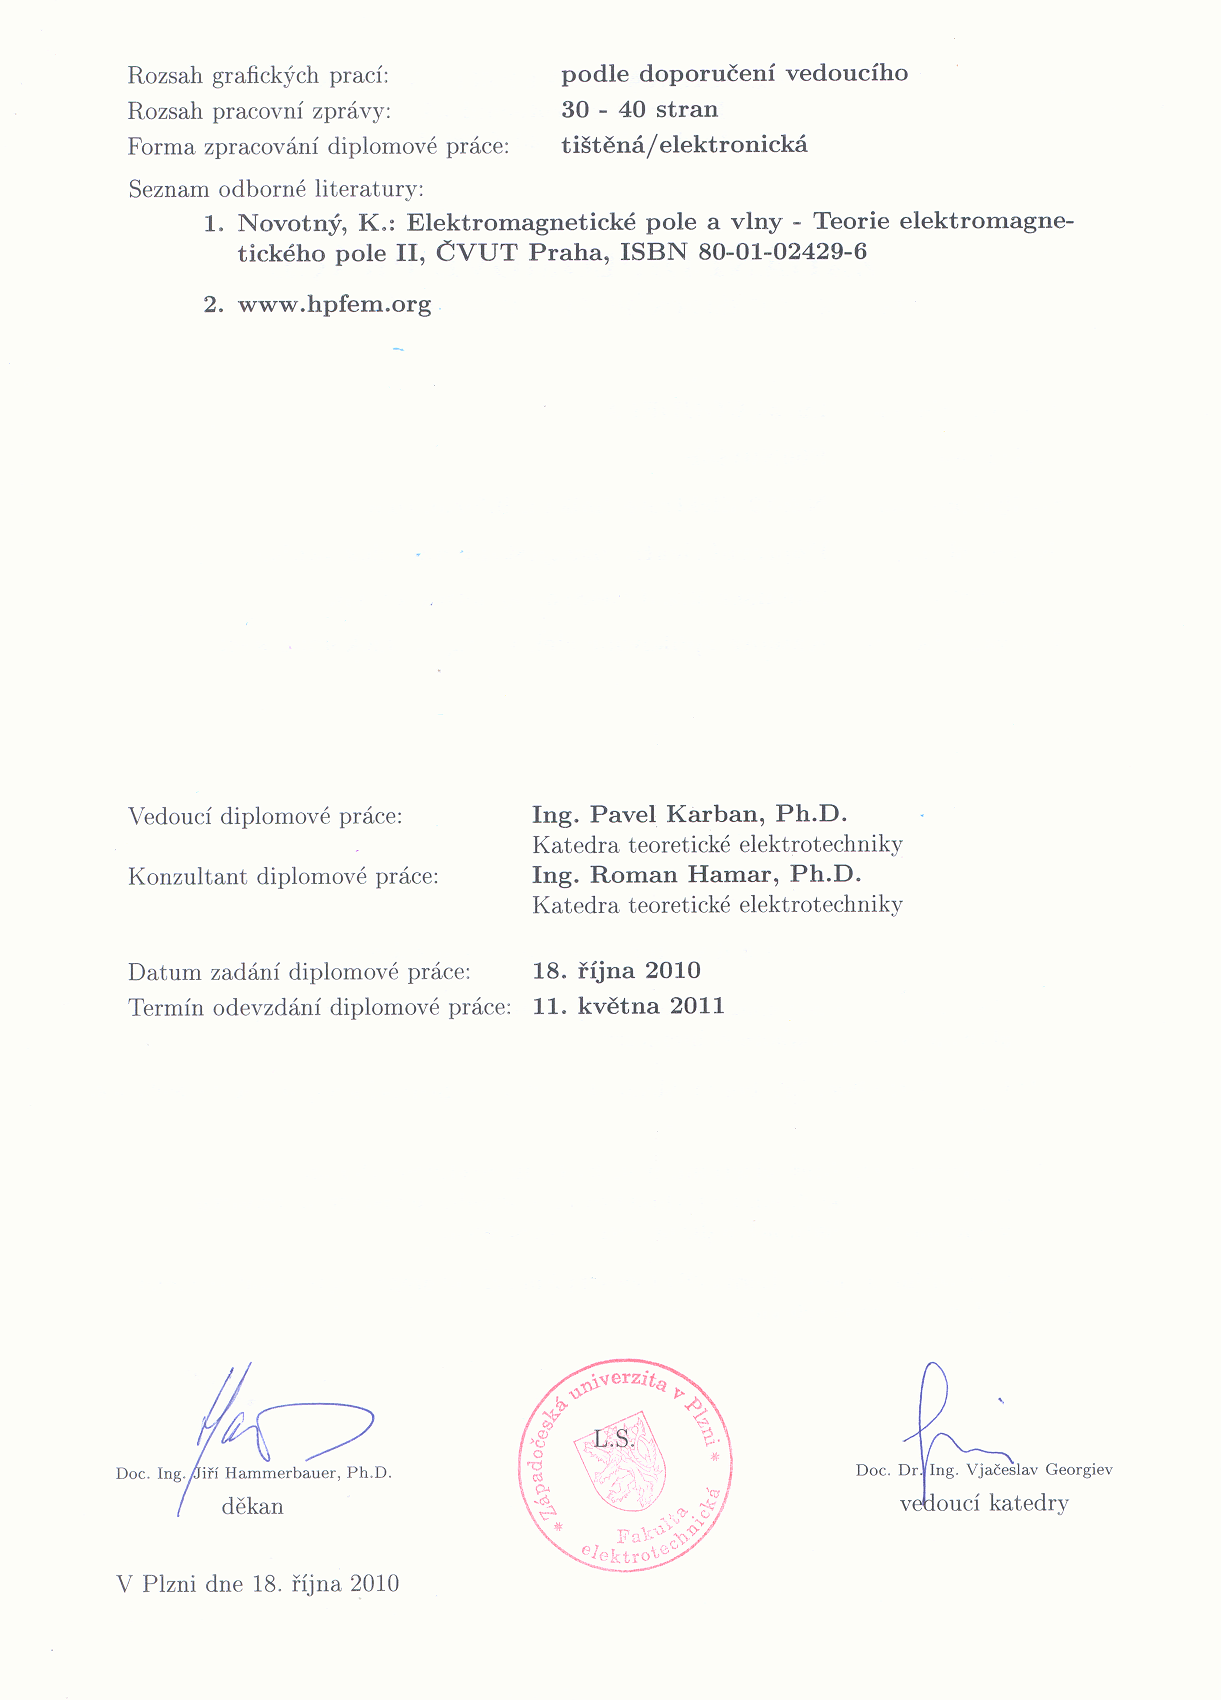
\includegraphics[width=15cm]{zadani2.png}
\end{figure}
\newpage

\section*{Anotace}
Diplomová práce se zabývá principem šíření elektromagnetických vln a jejich chování v~různých fyzikálních prostředích. Pojednává o~problematice elektromagnetické kompatibility v~elektrické trakci a uvádí související normy. Praktická část popisuje realizaci softwarové aplikace pro simulaci s~využitím knihovny Hermes2D.

\section*{Klíčová slova}
EMC, elektrická trakce, programovací jazyk C++,  Qt SDK, Hermes2D, Agros2D

\bigskip
% The Simulation of Electromagnetic Wales Propagation

\section*{Annotation}

The present thesis deals with the principle of electromagnetic waves propagation and their behavior in different physical environments. It discusses the issues of electromagnetic compatibility in electric traction and provides related standards. In the practical part, the realization of software application for simulation using the library Hermes2D is described.

\section*{Keywords}
EMC, Electric traction, programming language C++, Qt SDK, Hermes2D, Agros2D
\newpage

\section*{Prohlášení}
Předkládám tímto k~posouzení a obhajobě diplomovou práci zpracovanou na závěr studia na Fakultě elektrotechnické Západočeské univerzity v~Plzni.

\hyphenation{literatury}
Prohlašuji, že jsem diplomovou práci vypracoval samostatně s~použitím odborné literatury a pramenů uvedených v~seznamu, který je součástí této diplomové práce.
Dále prohlašuji, že veškerý software, použitý při řešení této diplomové práce, byl využit podle pravidel stanovených autorem.\bigskip \bigskip \\

\noindent V~Plzni, dne 23. dubna 2011 \hfill \ldots \ldots \ldots \ldots \ldots \ldots \ldots \ldots \ldots \ldots
\noindent \begin{flushright}Bc. Lukáš Koudela ~~~~~~~\end{flushright}
\newpage

\section*{Poděkování}
Na tomto místě bych rád vyjádřit poděkování vedoucímu diplomové práce Ing. Pavlu Karbanovi, Ph.D., a konzultantu Ing. Romanu Hamarovi, Ph.D., za veškeré cenné rady, konstruktivní připomínky, ochotu a čas, který mi při řešení problémů spojených s~touto prací věnovali.

\hyphenation{Mlsnové}
Také bych touto cestou chtěl poděkovat svým rodičům a přítelkyni Stanislavě Mlsnové za veškerou jejich nedocenitelnou podporu během studia. Bez jejich pomoci by tato práce nikdy nevznikla.\bigskip \bigskip \\

\noindent V~Plzni, dne 23. dubna 2011 \hfill \ldots \ldots \ldots \ldots \ldots \ldots \ldots \ldots \ldots \ldots
\noindent \begin{flushright}Bc. Lukáš Koudela ~~~~~~~\end{flushright}
\newpage
%% !TeX root = Main.tex
\chapter*{Seznam použitých symbolů}
\begin{tabular}{lll}
	$\vec{E}$ & $\unit V\cdot m^{-1}$ & intenzita elektrického pole\\
	$\vec{D}$ & $\unit C\cdot m^{-2}$ & elektrická indukcel\\
	$\vec{B}$ & $\unit T$ & magnetická indukce\\
	$\vec{H}$ & $\unit A\cdot m^{-1}$ & intenzita magnetického pole\\
	$\vec{J}$ & $\unit A\cdot m^{-2}$ & proudová hustota\\	
	$f$ & $\unit Hz$ & frekvence\\
	
	
	$\phi$ & $\unit Wb$ & magnetický indukční tok\\
	$i(t)$ & $\unit A$ & okamžitá hodnota elektrického proudu\\
	$I$ & $\unit A$ & maximální hodnota elektrického proudu, ss. elektrický proud\\
	$\omega$ & $\unit rad\cdot s^{-1}$ & úhlová frekvence\\

	$\vec{v}$ & $\unit m\cdot s^{-1}$ & rychlost\\

	$p_{\rm{J}}$ & $\unit W$ & Jouleovy ztráty\\
	$R$ & $\unit \Omega$ & elektrický odpor\\
	$a$ & $\unit m$ & hloubka vniku naindukovaných proudů\\
	$\gamma$ & $\unit S\cdot m^{-1}$ & elektrická vodivost\\
	$\mu$ & $\unit H\cdot m^{-1}$ & permeabilita\\
	$\mu_{\rm{r}}$ & $\unit -$ & relativní permeabilita\\
	$\mu_0$ & $\unit H\cdot m^{-1}$ & permeabilita vakua\\


	


	$\lambda$ & $\unit W\cdot m^{-1} \cdot K^{-1}$ & tepelná vodivost\\
	$T$ & $\unit \degree$ & teplota\\
	$\rho$ & $\unit kg\cdot m^{-3}$ & měrná hmotnost\\
	$c$ & $\unit J\cdot kg^{-1} \cdot K^{-1}$ & měrná tepelná kapacita\\
	$P$ & $\unit W$ & elektrický výkon, příkon\\
\end{tabular}
\renewcommand\thepage{}

%\tableofcontents
%\newpage

\renewcommand\thepage{\arabic{page}}
\setcounter{page}{1}
\pagenumbering{arabic}

%\chapter{Úvod}
%% !TeX root = Main.tex

V~posledních desetiletích se při vývoji nových zařízení nehledí jen na~to, aby daný výrobek plnil svojí primární funkci, pro kterou byl navržen, ale předmětem zájmu jsou také ostatní provozní vlastnosti. Mezi nejvýznamnější se řadí činnost bez vytváření nepřípustné úrovně elektromagnetického rušení a bezchybné fungování v~daném prostředí. Vědecká disciplína, která se danou problematikou podrobněji zabývá je označována pojmem elektromagnetická kompatibilita (z~anglického \uv{Electromagnetic Compatibility}, označované zkratkou EMC). Významnost tohoto specifického oborou narostla i díky rozvoji a rozšíření elektrotechniky, zvláště pak číslicové mikropočítačové elektroniky, která je dnes využita v řadě technických oblastí.

Existuje celá řada aplikací, ve kterých se šíření elektromagnetického pole může negativně projevovat. To se týká poměrně jednoduchých zapojení, složitějších analogových nebo digitálních obvodů, až komplexních procesorových systémů. EMC je v~této práci zaměřena na obor elektrické trakce, neboť v~tomto segmentu dochází k~častému prolínání řady systémů různých výkonů, topologií i principů činnosti. Nutno podotknout, že vliv elektromagnetických vln nemusí být vždy negativní. V~řadě aplikací představují vůbec základní element fungování. Typickým příkladem je oblast komunikací. Jedná o~využití radiových vln v~radiotechnice nebo při konkrétní konstrukci používaných zařízení, např. vlnovodů, rezonátorů.

Problematika elektromagnetické kompatibility zařízení velmi široce souvisí s~návrhem a konstrukcí. Především již ve fázi návrhu zařízení se uvažuje nad tím, v~jakém prostředí bude používané. V~řadě aplikací ale nelze z~provozních hledisek provádět funkční zkoušky prototypů v~konkrétním prostředí. Nejen z~tohoto důvodu narůstá význam simulačních aplikací, díky kterým je možné předem nasimulovat např. schopnost použitého stínění nebo účinnost navržené antény. Mezi další přínosy může přirozeně patřit urychlení vývoje nebo snížení nákladů na výrobu. Právě tvorba aplikace pro možnost simulace elektromagnetického pole je ústředním tématem této diplomové práce. Konkrétněji o~tom pojednává kapitola \ref{kap:Cile}.

Práce je složena z~několika kapitol. Kapitola \ref{kap:Cile} vytyčuje konkrétní cíle, které tato práce hodlá splnit, kapitola \ref{kap:EMC} se s pomocí \cite{emc_trakce}, \cite{nfr}, \cite{emc_encyklopedie} a \cite{csn} zabývá problematikou EMC v~konkrétním technickém oboru, v~elektrické trakci. V~další kapitole \ref{kap:Evlny} je dle \cite{emp}, \cite{umt} a \cite{tripak} rozebrán matematický popis elektromagnetických vln a popsáno jejich chování v~různých fyzikálních prostředích. Návrhem aplikace pro simulace šíření elektromagnetických vln se s využitím \cite{num}, \cite{hpfem}, \cite{gk_kaw} a \cite{gk_tichy} zabývá kapitola \ref{kap:Simulace}, ilustrativní příklad řešení je popsán v kapitole \ref{kap:Priklad}. V~závěrečné kapitole \ref{kap:Zaver} jsou shrnuty dosažené poznatky a popsány výsledky práce. V~příloze \ref{kap:Odvozeni_VlnR}~se nachází podrobné odvození vlnových rovnic elektromagnetického pole, v příloze \ref{kap:tutorial} je popis řešení úloh v aplikaci Agros2D. Příloha \ref{kap:Program_kod} je shrnutím nejdůležitější částí programového kódu simulačního modulu.



%\chapter{Cíle práce} \label{kap:Cile}
%% !TeX root = Main.tex
Vznik tématu této diplomové práce souvisí s~vývojem aplikace Agros2d na Katedře teoretické elektrotechniky Fakulty elektrotechnické Západočeské univerzity v~Plzni. Tento univerzální multiplatformín program distribuovaný pod GNU/GPL licencí slouží k~řešení fyzikálních polí. Umožňuje simulaci elektrostatického, elektrického proudového, magentického nebo teplotního pole. Hlavním přínosem v~rámci diplomové práce bude s~využitím knihovny Hermes2D doplnění dalšího fyzikálního pole, které bude zobrazovat chování elektromagnetického pole popsané vlnovými rovnicemi. Práce si tedy klade za cíl především doplnit vyvíjenou aplikace od další modul, čímž by rozšířila možnosti jeho použití do dalších technických oborů. 

Dalším účelem je nasimulovat vybrané vlnové problémy pro účely výuky předmětu KTE/EV. Jedná se o~příklady, šíření elektromagnetických vln na dipólu, na rozhraní dvou prostředí, ve vrstveném prostředí, ve vlnovodných strukturách a v~dutinových rezonátorech.


%\chapter{EMC v~elektrické trakci} \label{kap:EMC}
%% !TeX root = Main.tex
\section{Souvislost EMC a elektrické trakce} \label{sec:emc_trakce}
Elektrická trakce je velmi specifickou oblastí. Problematika elektromagnetické kompatibility je zde obsáhlá, neboť se týká nejen situace ohraničené prostorem vlakových souprav, ale i~dalších propojených oblastí. Prolínají se tu elektrické systémy velmi vysokých výkonů, nelineární výkonové elektronické prvky i systémy dopravně signalizační a zabezpečovací. Mezi konkrétní odlišnosti u~drážních zařízení patří dle \cite{nfr} například:
\begin{itemize}
\item Topologie trakčního vedení (jednostranně, maximálně oboustranně napájené).
\item Lokomotiva představuje jednofázovou zátěž o~značném výkonu v~řádech tisíců kW (např. ŠKODA 109 E poskytuje jmenovitý výkon $6400 \unit{kW}$)
\item Proměnná vzdálenost mezi napájecí stanicí a místem odběru (s~tím související variabilita parametrů vedení)
\end{itemize}
Dle \cite{emc_trakce} je na problematiku EMC v~elektrické trakci nahlíženo komplexně a rozděluje se dle kmitočtových pásem na 2 oblasti:

\medskip
{\bf Nízkofrekvenční rušení} (frekvenční pásmo 0 až 2500 Hz) \\
Zdrojem rušení představují především polovodičové měniče. Ty během své činnosti vytvářejí vyšší harmonické proudy. Vzhledem k~rozsahu provozovaných výkonů se jedná o~nezanedbatelnou složku v~trakčním napájecím vedení. Důsledkem tohoto typu rušení je zvýšení odběru jalového a deformačního výkonu, čímž dochází k~souvisejícímu zhoršení celkového účiníku $\lambda$ (označovaný jako \uv{power factor}). Vliv vyšších harmonických proudů nelze nikdy úplně odstranit, ale je možné snížit jejich účinky. To se týká především omezením velikostí proudů konstrukcí měničů, metodami řízení, doplňkovou výbavou či dalšími kompenzačními zařízeními a filtry. O~daných prostředcích je blíže pojednáno v~\cite{nfr}.

\medskip
{\bf Vysokofrekvenční a impulsní rušení} (frekvenční pásmo 9 kHz až 1 GHz) \\
V~této kmitočtové oblasti jsou předmětem zájmu impulsy, které vznikají při spínacích pochodech v~napájecích stanicích, případně v~lokomotivách. Zdroje tohoto rušení mohou nepříznivě až kriticky ovlivňovat, kromě všech drážních zařízení, také blízké okolí rozvodů trakčního vedení. Mezi obzvláště citlivé spotřebiče na rušivé vlivy od elektromagnetického pole lze považovat zařízení komunikací, sdělovací systémy a veškerá řídící technika, realizovaná v~dnešní době procesorovou a číslicovou elektronikou. O~úrovních přípustného rušení v~elektrické trakci je pojednáno v~příslušných normativech, které jsou popsány v~podkapitole \ref{sec:emc_normy_trakce}. Omezení vlivu elektromagnetického pole na dané zařízení je možné pomocí stínění, k~jehož návrhu a realizaci je často vhodné využít simulačních aplikací. Více o~realizaci nástroje pro simulaci pojednává kapitola \ref{kap:Simulace}.
\newpage

\section{Dělení EMC a struktura norem}
Rozdělení příslušných norem souvisí s~tím o~jakou konkrétní oblast elektomagnetické kompatibility se jedná. U~technických systémů jsou oblasti rozčleněny dle působení a~definuje se základní přenosový řetězec. V~této podkapitole je využito zdrojů \cite{nfr} a \cite{emc_encyklopedie}.
\begin{figure}[!h]
	\centering
	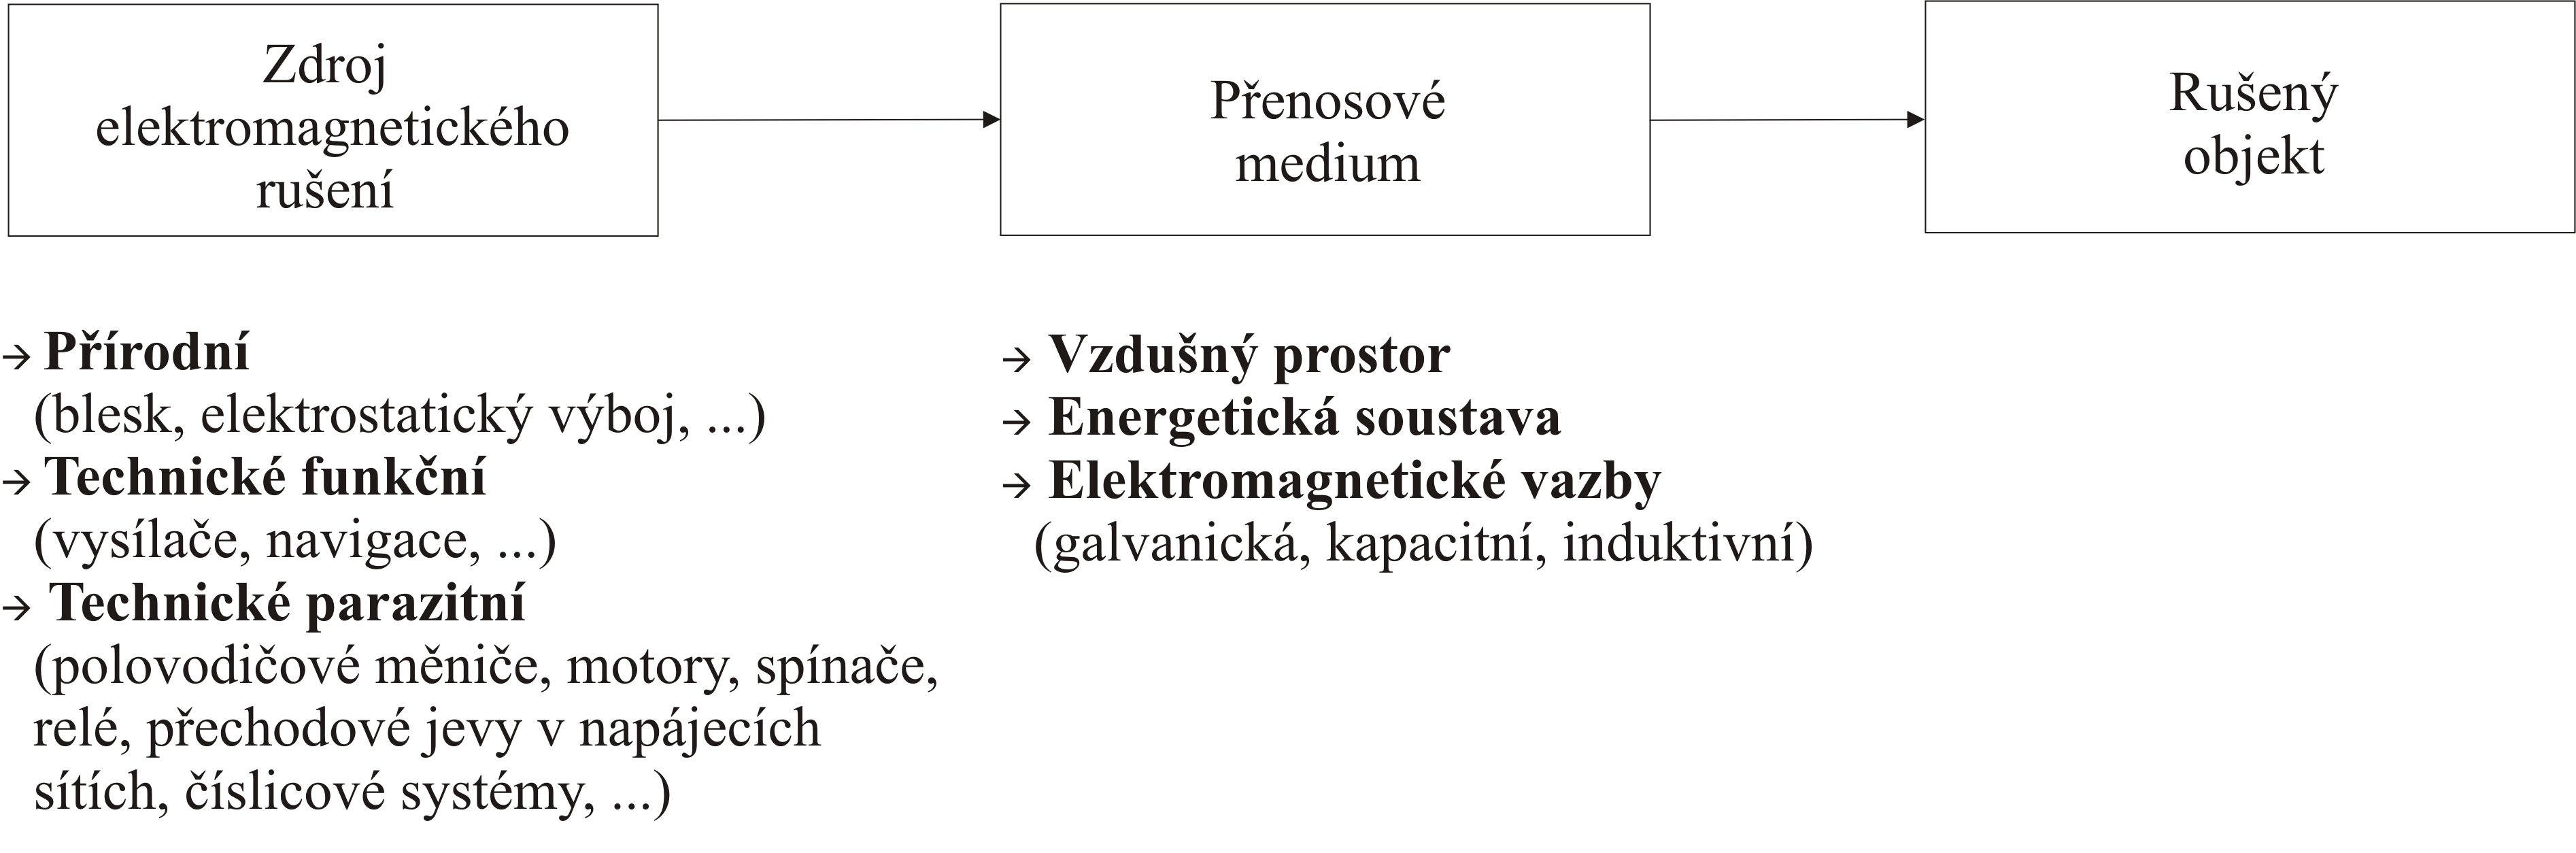
\includegraphics[width=14.6cm]{emc_retezec.png}
	\caption{Přenosový řetězec EMC a příklady jednotlivých bloků.}
	\label{obr:emc_retezec}
\end{figure}\\
Základní rozdělení EMC se zabývá:
\begin{itemize}
\item {\bf EMI} - Elektromagnetická interference (zdroj elektromagentického rušení). \\
Tato oblast se věnuje prvnímu bloku na obr. \ref{obr:emc_retezec}. Zabývá příčinami vzniku rušení, dále parametry, intenzitou, charakterem a také například možnostmi jeho měření. Interferenční zdroje se rozdělují na přírodní a na technické, neboli umělé. U~těch se ještě blíže rozlišuje, zda se jedná o~požadovanou funkci vysílače nebo nechtěnou. Konkrétních zdrojů, především pak technických, existuje nepřeberné množství z~nichž některé jsou uvedeny u~přenosového řetězce.

Dále se musí blíže specifikovat, zda se jedná o~přímý vliv elektromagnetického pole nebo jde o~rušení po vedení. Levá část obrázku \ref{obr:emc_emi_ems} znázorňuje rozdíl mezi vyzařováním a~šířením rušivých vlivů po napájecím vedení.

\item {\bf EMS} - Elektromagnetická susceptibilita (odolnost rušeného objektu). \\
Schopnost odolat vlivu elektromagnetického rušení se sleduje u~posledního bloku na obrázku \ref{obr:emc_retezec}. Tím jsou konkrétní zařízení nebo systémy, které jsou vystaveny přímému vlivu elektromagnetického pole. Případně mohou být ohroženy rušením po napájecím vedení, tak jak je naznačeno na obrázku \ref{obr:emc_emi_ems}.
\end{itemize}
\begin{figure}[!h]
	\centering
	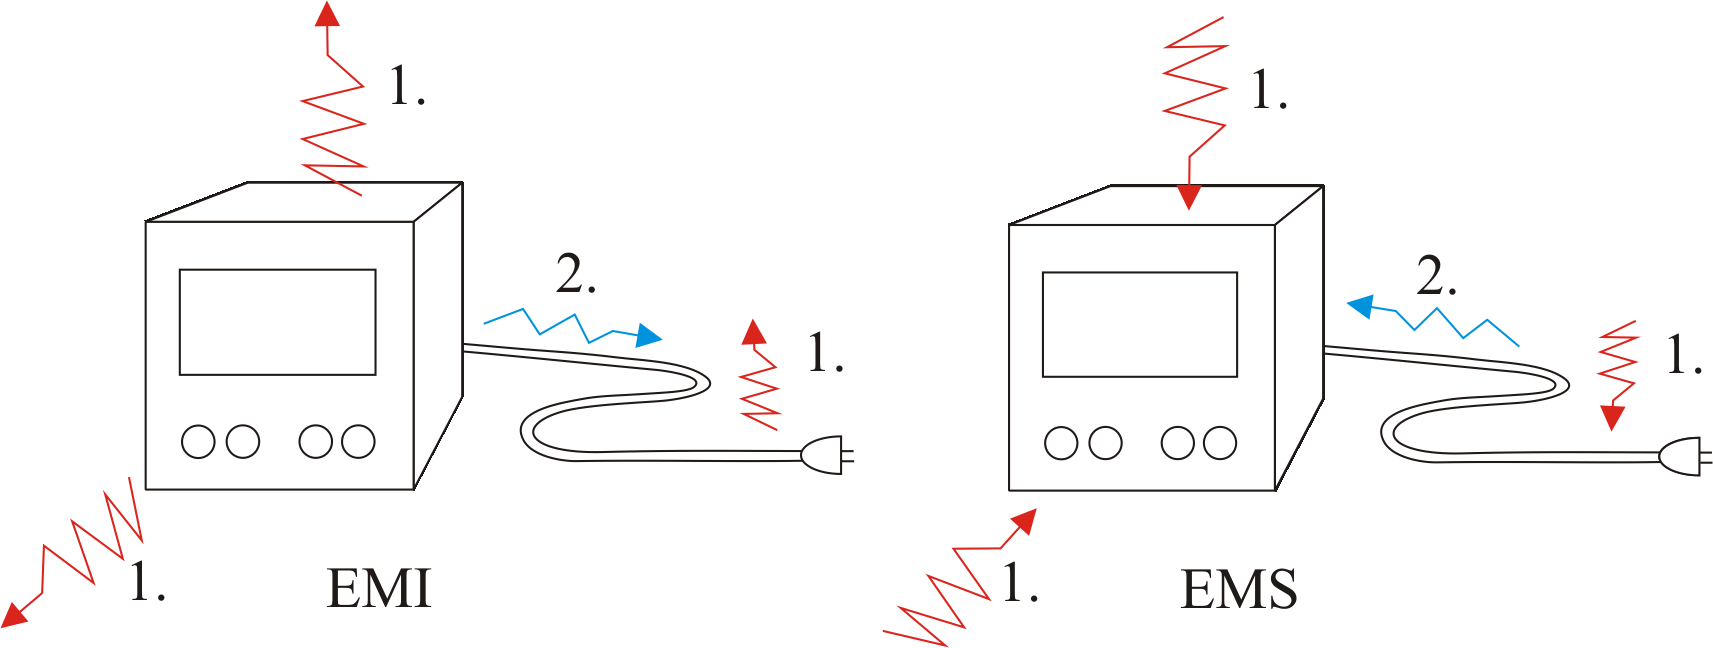
\includegraphics[width=10.5cm]{emc_emi_ems.png}
	\caption{EMI a EMS zářením (1.) a šířením po vedení (2.).}
	\label{obr:emc_emi_ems}
\end{figure}

Úrovně EMI a EMS jsou rozhodující pro návrh a konstrukci zařízení. Aby daný výrobek byl provozuschopný z~hlediska elektromagnetické kompatibility, je potřeba splňovat podobné úrovně rušení jako je nastíněno na obrázku \ref{obr:emc_meze}. To především znamená, že elektromagnetická odolnost daného zařízení by měla být dostatečně dimenzovaná, aby ji nepřesáhl nějaký zdroj rušení vyskytující se v~daném prostředí. Dle norem jsou definované hodnoty pro EMS a EMI, které představují rezervy pro zajištění EMC.
\begin{figure}[!h]
	\centering
	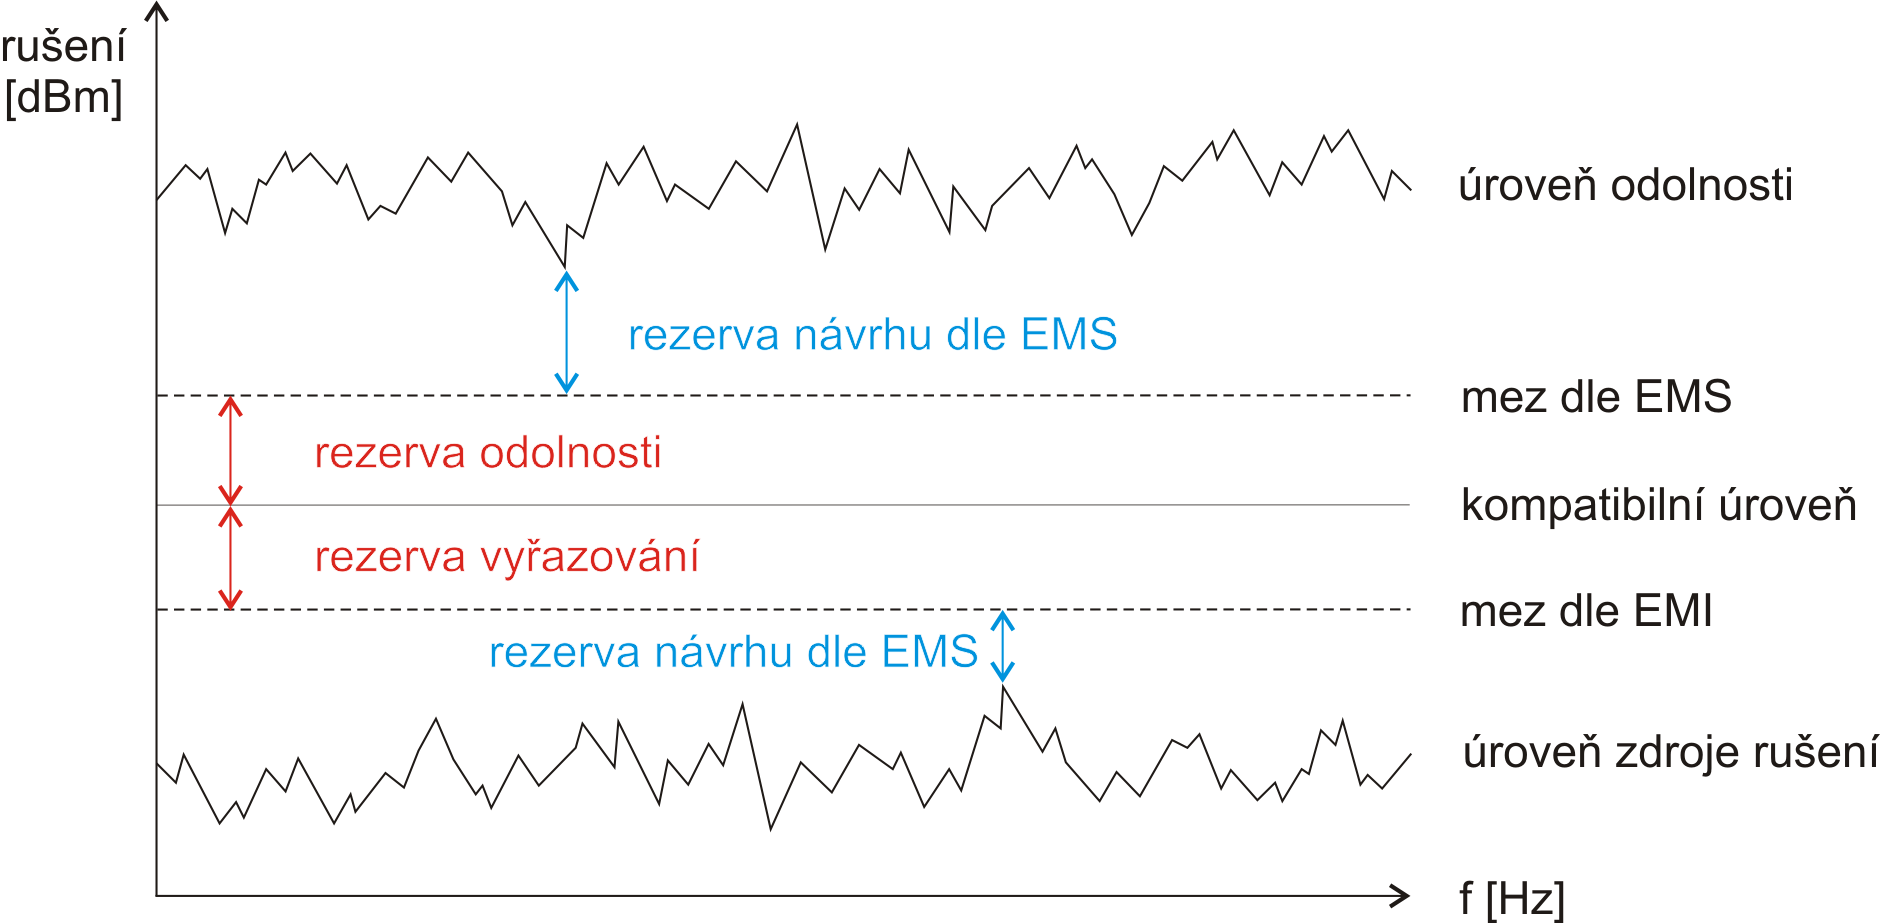
\includegraphics[width=11cm]{emc_meze.png}
	\caption{Vliv úrovní EMI a EMS pro konstrukci zařízení.}
	\label{obr:emc_meze}
\end{figure}

Účelem předpisů EMC je hlavně zvýšení elektromagnetické kompatibility systémů. Toho lze dosáhnout právě omezováním zdrojů rušení ze současného zvyšování odolnosti objektů. Civilní normy EMC se dle charakteru rozlišují na:
\begin{itemize}
\item {\bf Základní} (Basic Standarts) - Specifikují všeobecné podmínky pro dosažení elektromagnetické kompatibility u~libovolného technického zařízení.
\item {\bf Kmenové} (Generic Standarts) - Definují bližší kritéria na EMI a EMS podle typu prostředí, ve kterém je dané zařízení trvale provozováno.
\item {\bf Výrobků} (Product Standarts) - Určují detailní požadavky a testovací metody pro produkty nebo skupiny podobných produktů. Do této kategorie spadají také normy pro elektrickou trakci, které jsou rozepsány v~podkapitole \ref{sec:emc_normy_trakce}.
\end{itemize}
V~tabulce \ref{tab:emc_deleni} je uvedeno další obecnější rozdělení, podle kterého je možné členit normy elektromagnetické kompatility. Pro příslušnou oblast jsou definovány dvě části norem. V~první bývají uvedeny meze EMC a v~druhé se nacházejí postupy pro testování.
\begin{table}[!h]
\begin{center}
  	\caption{Obecné rozdělení norem EMC.}
  	\label{tab:emc_deleni}
\begin{tabular}{|l|l|}
	\hline
	{\bf Pokrytá oblast}  & {\bf Části norem} \\
	\hline
	\hline
	Normy rušivého vyzařování  (pro EMI) & mezní (maximální) hodnoty vyzařování \\
	 & měřící přístroje a metody \\
	\hline
	Normy elektromag. odolnosti  (pro EMS) & mezní (minimální) hodnoty odolnosti \\
	 & zkušební přístroje a metody \\
	\hline
	Normy odrušovacích prostředků  & vlastnosti odrušovacích prostředků \\
	 & zkoušky a přístroje pro měření \\
	\hline
\end{tabular}
\end{center}
\end{table}
\newpage

\section{Aktuální normativy v~elektrické trakci} \label{sec:emc_normy_trakce}
Mezi aktuální normy, související s~elektromagnetickou kompatibilitou v~elektrické trakci, patří především České technické normy s~označením ČSN EN 50121 \cite{csn}. Jedná se o~překlady, které zajišťuje Český normalizační institut. Mají proto stejný statut jako oficiální verze, kterými jsou evropské normy EN 50121, vydávané Evropským výborem pro normalizaci v~elektrotechnice (CENELEC). 

Z~řady důvodů, jak provozních, tak i bezpečnostních, je elektromagnetická kompatibilita vážným problémem již při návrhu a následné konstrukci trakčních vozidel. Proto je nutné vytvořit normy, které budou splňovat jak veškeré požadavky Směrnice elektromagnetické kompatibility EC 89/336/EEC, tak i zajišťovat spolehlivost a funkčnost vlastních drážních zařízení.

Soubor norem ČSN EN 50121, vydaný pod společným názvem Drážní zařízení – Elektromagnetická kompatibilita, je rozčleněn na šest logicky souvisejících částí. Bylo by neúčelné vypisovat veškerá specifika, tabulky a grafy, které jsou v~těchto normách uvedené, proto se tato práce úzce zaměřuje pouze na hlavní oblast zájmu, kterého se daný normativ týká. Přesnější informace je možné získat nahlédnutím do příslušného dokumentu. \bigskip \\
Část 1: Všeobecně\\
Část 2: Emise celého drážního  systému do vnějšího prostředí\\
Část 3-1: Drážní vozidla – Vlak a celkové vozidlo\\
Část 3-2: Drážní vozidla – Zařízení\\
Část 4: Emise a odolnost zabezpečovacích a sdělovacích zařízení\\
Část 5: Emise a odolnost pevných instalací a zařízení trakční napájecí soustavy\\

\subsection{ČSN EN 50121-1}
Norma ČSN EN 50121-1: Všeobecně popisuje rozdělení celého vlastního souboru norem, jak je uvedeno v~části \ref{sec:emc_normy_trakce}. Dále obsahuje postupy pro řízení managementu pro dosažení EMC v~elektrické trakci. Nakonec především stanovuje funkční kritéria, které jsou založeny na evropské normě EN 61000-6-2. S~jejich pomocí se posuzuje funkčnost a~schopnost provozu zařízení během zkoušek EMC. V~normě jsou definována tři funkční kritéria, označovaná jako A, B a C. Pokud testovaný vzorek není schopen splnit požadavky alespoň jednoho z~uvedených kritérií, posuzuje se jako nevyhovující.

Funkční kritérium A~ve většině případů nedovoluje žádnou změnu chování zařízení během i následně po skončení zkoušek EMC. Jedinou modifikací může být výrobcem nastavená minimální hranice fungování, případně přípustná mez ztráty funkčnosti, které výrobek, během testů a po nich, přesto nesmí překročit.

Funkční kritérium B nedovoluje zhoršení funkce po ukončení zkoušek, pokud je zařízení používáno podle svého určení. Během testů je však akceptovatelné zhoršení činnosti. To lze za předpokladu, že se nezmění současný provozní stav a nedojde ke ztrátě dat v~paměti zařízení.

Funkční kritérium C popisuje, že u~zkoušeného zařízení je možná dočasná ztráta funkce, pokud je nějakým prostředkem možno zajistit její obnovení.

\subsection{ČSN EN 50121-2}
Norma označená ČSN EN 50121 - 2: Emise celého drážního  systému do vnějšího prostředí ustanovuje mezní hodnoty emisí, které mohou být produkovány při provozu drážních vozidel. Dále určuje, jakým způsobem měření lze dané hodnoty ověřit. Dle normy se předpokládá, že elektromagnetické rušení působené elektrickou trakcí, existuje ve všech místech ve vzdálenosti 10 m od vnější elektrizované troleje nebo 10 m od trakční napájecí stanice. I proto je stanoveno provádět měření emisí v~této vzdálenosti. Pokud není možné tuto podmínku vzhledem k~místním poměrům na dráze dodržet, existuje v~normě definovaný přepočet pro měření v~jiné ekvivalentní vzdálenosti. 

Mezní hodnoty se podle normy rozlišují na vyzařování z~venkovní dráhy při provozu vlaku a samostatně na emise z~trakčních napájecích stanic. Hranice (velikost vrcholové případně kvazivrcholové hodnoty) pro jednotlivé napájecí systémy v~elektrické trakci používané v~České republice jsou uvedeny v~grafu na obrázku \ref{obr:emc_emise}.

\begin{figure}[!h]
	\centering
	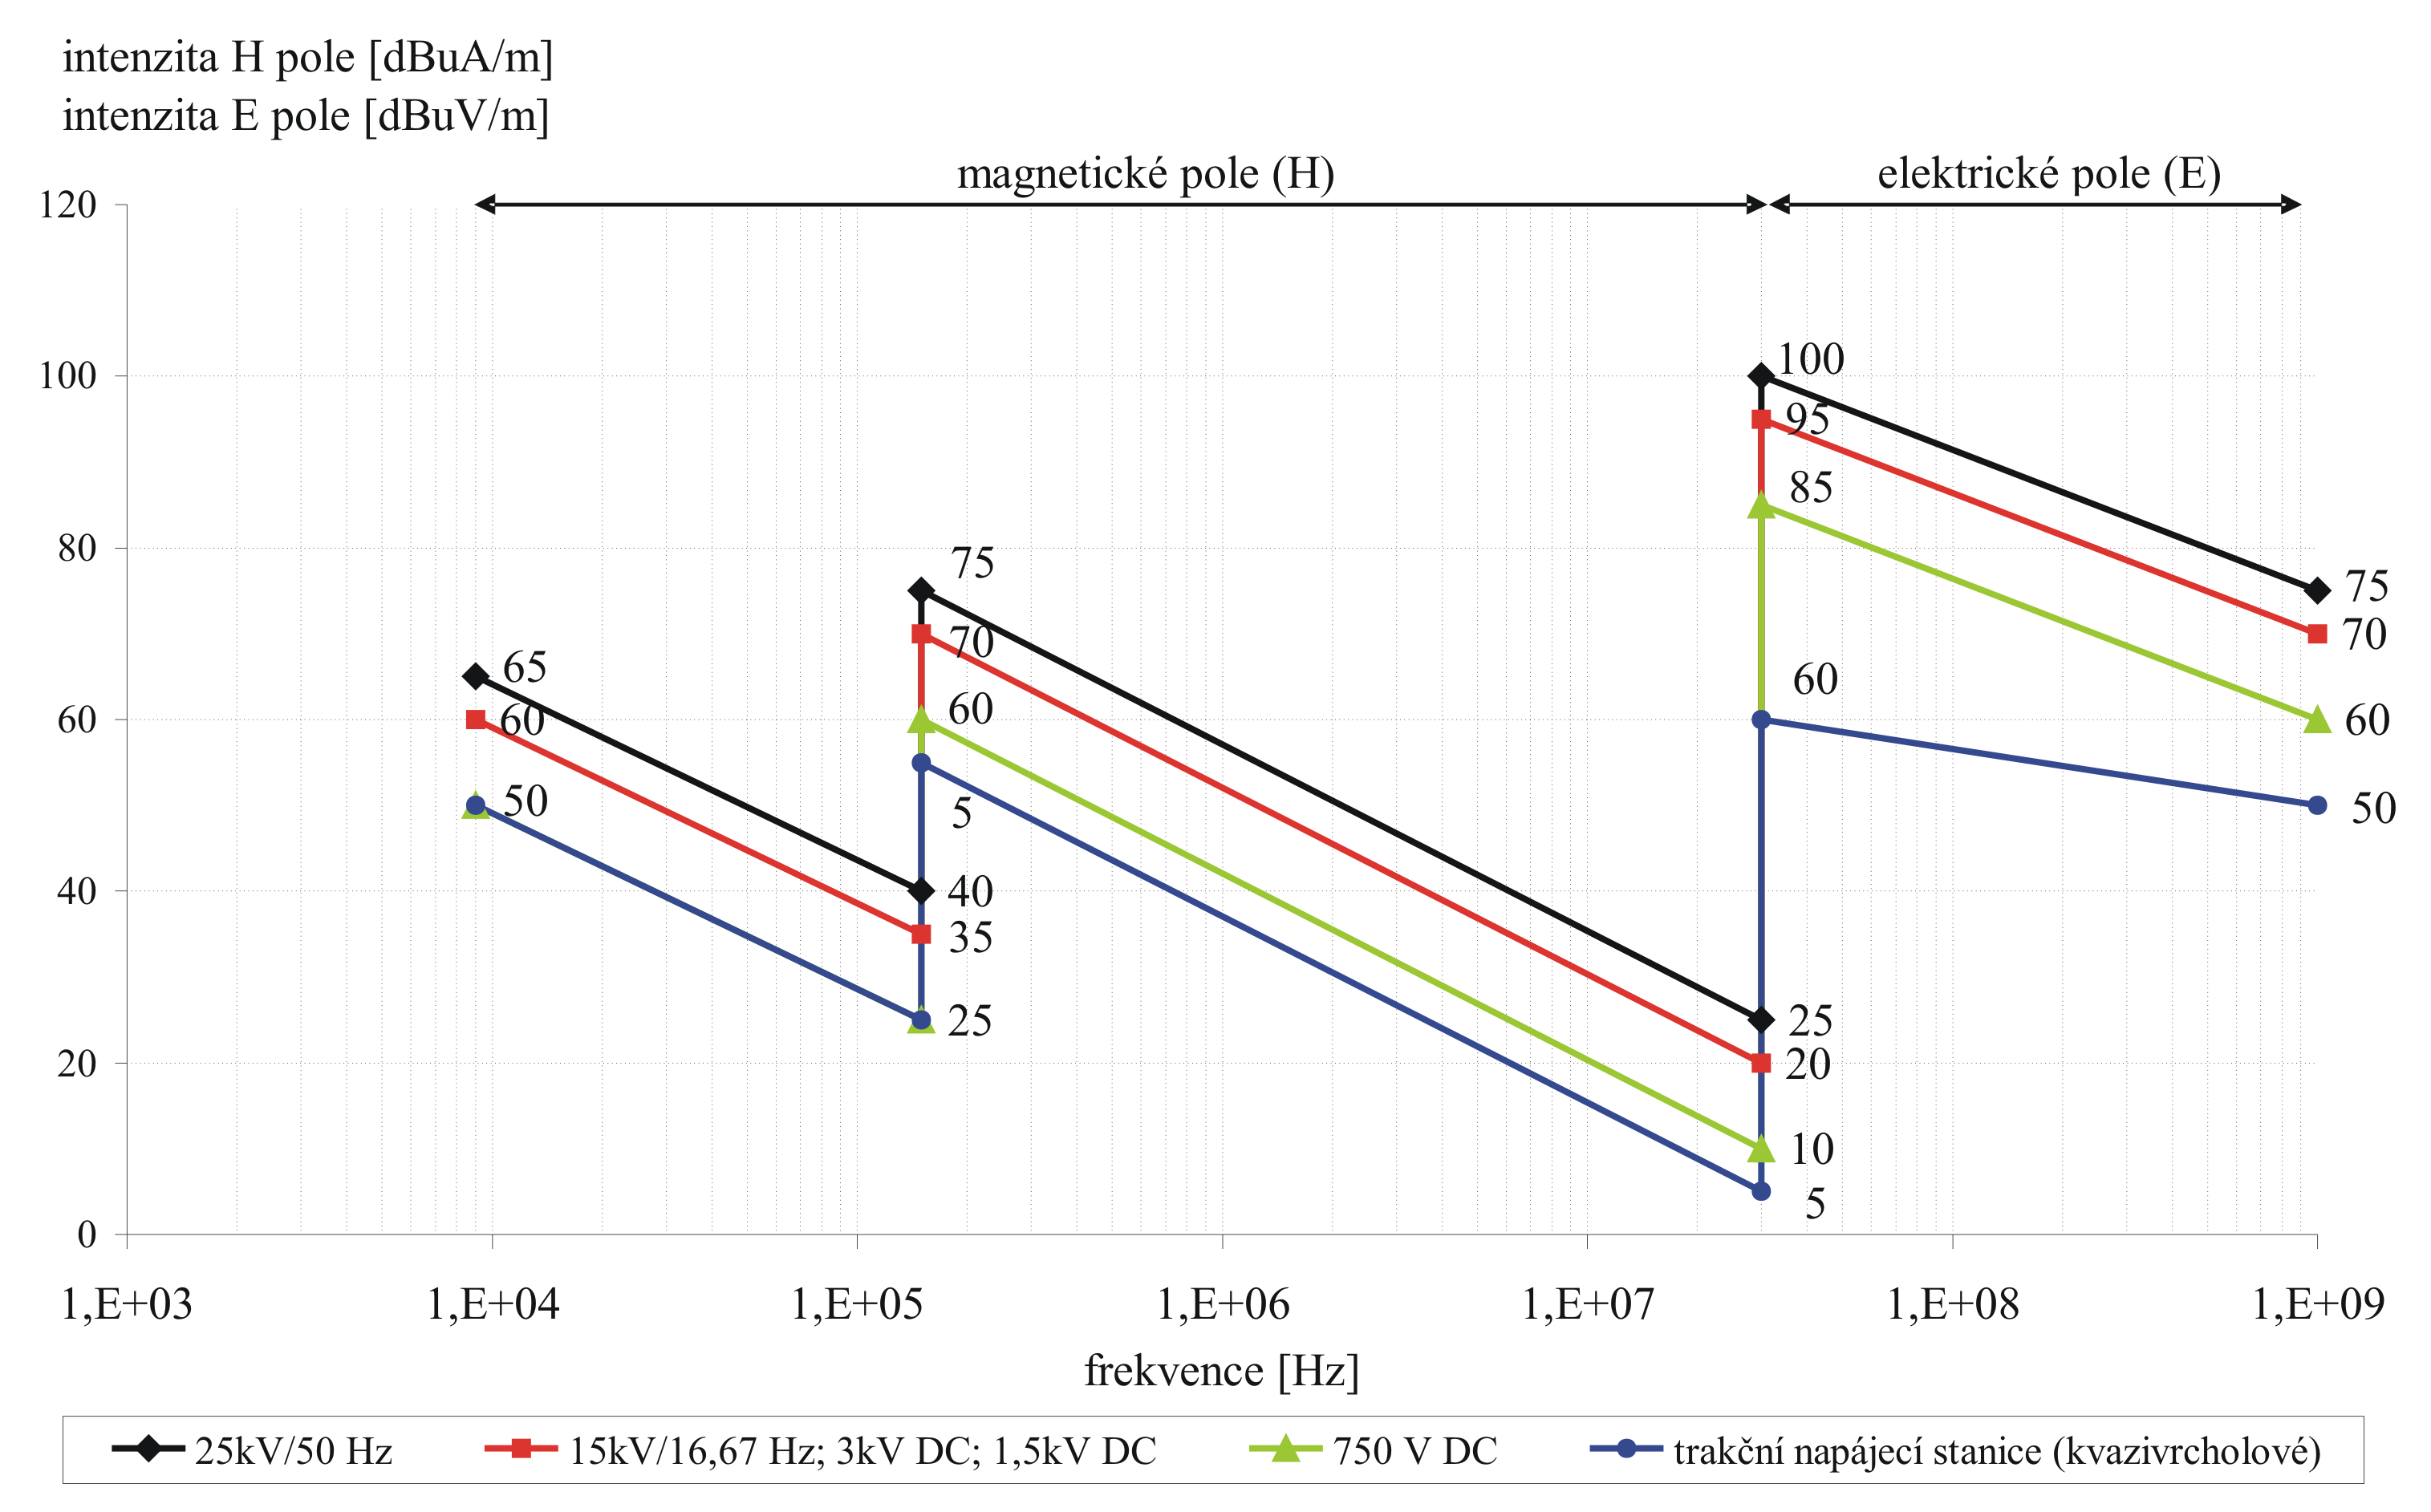
\includegraphics[width=12cm]{emc_emise.png}
	\caption{Hranice emisí jednotlivých trakčních systémů v~pásmu 9 kHz až 1 GHz.}
	\label{obr:emc_emise}
\end{figure}

Vlastní měření intenzity elektromagnetického pole, generovaného drážními vozidly, se provádí detektorem vrcholové hodnoty ve vzdálenosti 10 m od osy koleje. Určuje se horizontální magnetická složka pole (kolmá k~trati). U~elektrické složky vyzařovaného pole se měří složka vertikální a horizontální (rovnoběžná s~tratí). Normou definované šířky pásma pro pokles měřené veličiny o~6 dB  a použité měřící zařízení pro pokrytí celého kmitočtového pásma jsou uvedeny v~následující tabulce \ref{tab:emc_fr_rozsah}.

\begin{table}[!h]
\begin{center}
  	\caption{Přehled měřených frekvenčních rozsahů a měřících antén.}
  	\label{tab:emc_fr_rozsah}
\begin{tabular}{|l|l|l|l|}
	\hline
	{\bf Kmitočtový rozsah} & {\bf Pásmo} & {\bf Měřící anténa} & {\bf Měřená složka pole} \\
	\hline
	\hline
	9 kHz - 150 kHz	& 200 Hz	& smyčková nebo rámová	& magnetická (intenzita $\vec H$) \\
	150 kHz - 30 MHz	& 9 kHz	& smyčková nebo rámová	& magnetická \\
	30 MHz - 300 MHz	& 120 kHz	& bikónický dipól		& elektrická (intenzita $\vec E$) \\
	300 MHz - 1 GHz	& 120 kHz	& logaritmicko - periodická	& elektrická\\
  	\hline
\end{tabular}
\end{center}
\end{table}

\subsection{ČSN EN 50121-3-1}
Další platnou normou souboru Drážní zařízení – Elektromagnetická kompatibilita je ČSN EN 50121-3-1: Drážní vozidla – Vlak a celkové vozidlo. Týká se všech hnacích prostředků, včetně městských drah a ucelených vlakových souprav, ale rozsah platnosti této normy končí na rozhraní vozidla. Tím se rozumí buď kluzný kontakt s~trolejovým vedením nebo přívodní kolejnicí, případně konektor AC nebo DC napájení u~tažených vozidel. Předmětem této normy je stanovení zkušebních podmínek a mezí pro elektromagnetickou emisi a odolnost, aby tím bylo zajištěno fungování trakčního vozidla v~jeho definovaném prostředí. 

Zkoušky emisí jsou vykonávány při provozních stavech, při kterých se předpokládá nejvyšší produkovaná hodnota elektromagnetického rušení. Uvedené mezní hodnoty odpovídají emisím v~normě ČSN EN 50121-2, které jsou uvedeny na obrázku \ref{obr:emc_emise}.

Zkoušky odolnosti se neprovádějí, normou je pouze stanovena pevná hranice 20~V/m v~kmitočtovém rozsahu 0,15 MHz – 2 GHz , do které se považuje vozidlo za odolné.

\subsection{ČSN EN 50121-3-2}
Normativ ČSN EN 51231-3-2: Drážní vozidla – Zařízení definuje elektromagnetické poměry pro veškerá zařízení, které je možné používat na trakčním vozidle, tak aby byla zajištěna bezproblémová činnost při všech provozních stavech. Je zde definována řada specifických požadavků. Například tato norma neplatí pro přechodné emise při vypnutí nebo zapnutí zařízení. Zvláštní požadavek platí pro prostředky radiokomunikací, pro které emise a odolnosti uvedené v~této normě neplatí. Pokud se jedná o~komponentu, kterou je potřeba připojit do systému vlastního vozidla, provádějí se veškeré zkoušky v~zapojeném stavu. Měření se navíc provádí pro všechny příslušné vstupy a výstupy. 
Rozlišují se na několik druhů, hlavní jsou uvedeny na obrázku \ref{obr:emc_IO}.

\begin{figure}[!h]
	\centering
	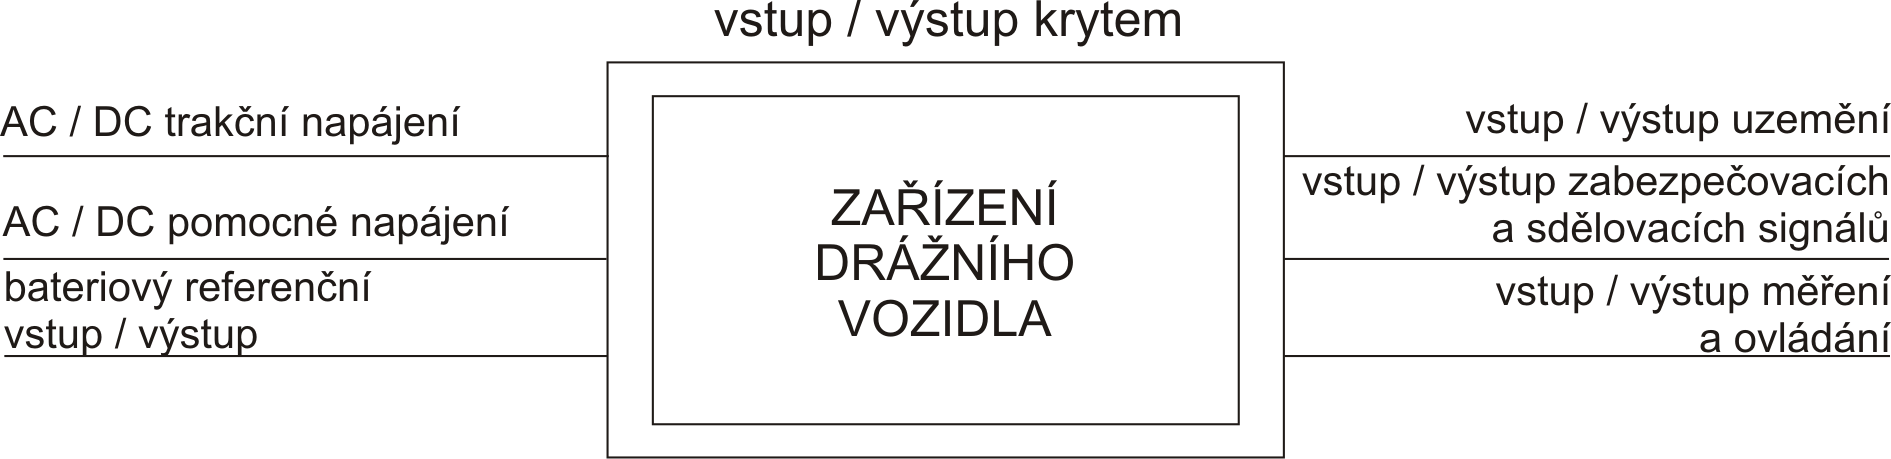
\includegraphics[width=11cm]{emc_IO.png}
	\caption{Hlavní druhy vstupů a výstupů zařízení. \cite{csn}}
	\label{obr:emc_IO}
\end{figure}

Pro veškerá měřená zařízení se určují funkční kritéria, které jsou definované v~ČSN EN 50121-1, tj. A, B a C. Norma také definuje postup pro měření vysokofrekvenčního rušení přenášené po přívodním vedení v~pásmu 9 kHz až 30 MHz, které je vytvářeno především napájecími měniči trakčních motorů (obecně přístrojů se spínanými zdroji). Princip zkoušky je naznačen na obrázku \ref{obr:emc_vf}. 

\begin{figure}[!h]
	\centering
	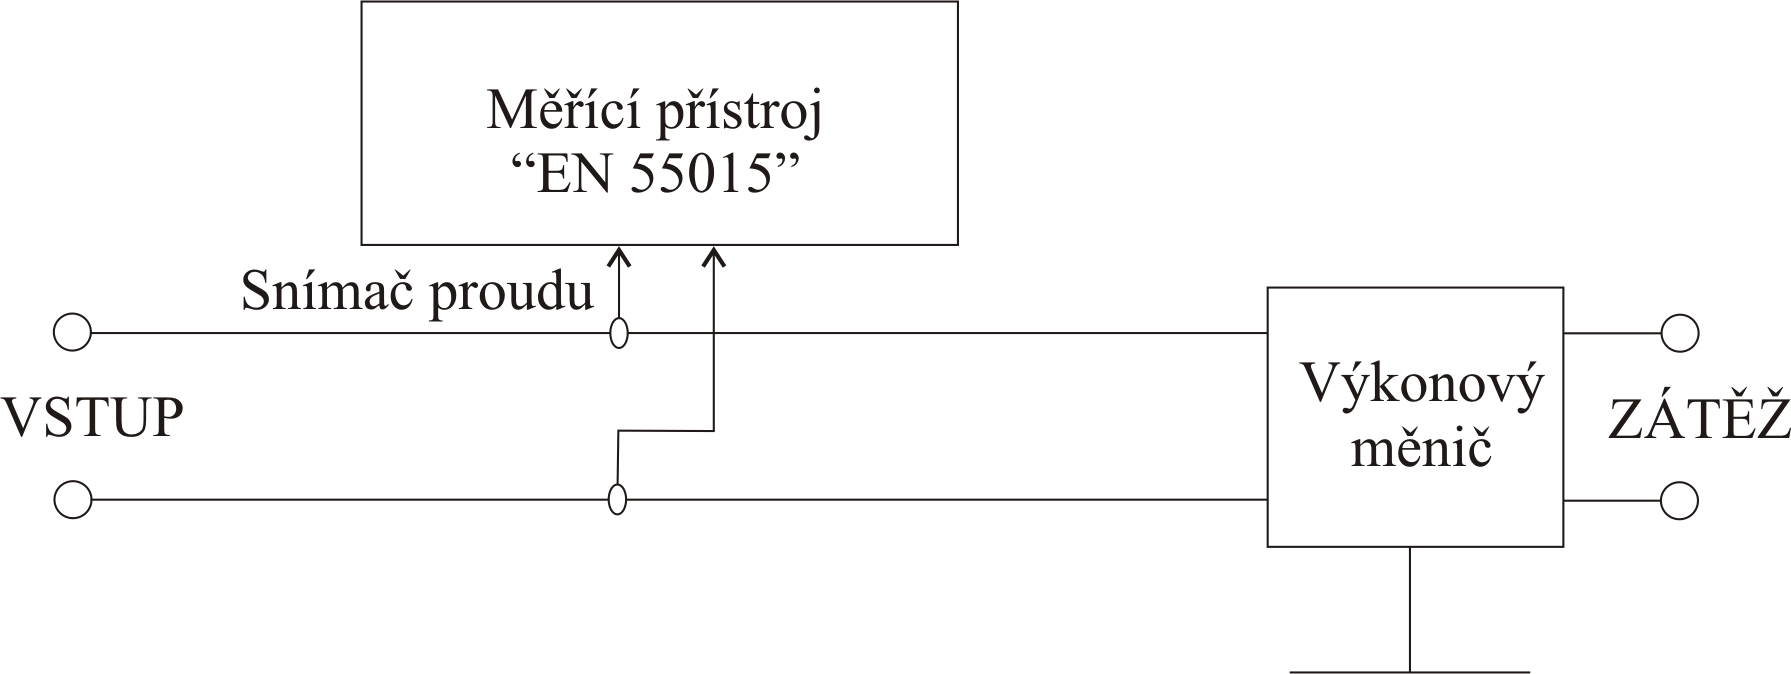
\includegraphics[width=8cm]{emc_vf.png}
	\caption{Zkouška vysokofrekvenčního rušení trakčních měničů. \cite{csn}}
	\label{obr:emc_vf}
\end{figure}

Úrovně rušení se určují v~řadě měřících bodů po celé délce vedení a vyhodnocují se maximální rušivé proudy. Aby měření nebylo ovlivněno trakčním proudem, je potřeba zajistit správné impedanční přizpůsobení mezi snímačem proudu a měřícím přístrojem. Meze emisí pro rušení po vedení u~tohoto měření nastaveny nejsou, pokud se jedná o~samostatné zařízení. Pokud je instalováno v~okolí jiného přístroje, musí vyhovovat mezním hodnotám vyzařování dle normy ČSN EN 50121-3-1.

Zkoušky odolnosti jsou touto normou specifikovány pro zkoušky postupného testování v~libovolném pořadí. Popis metod a odkazy na základní normy pro vstupy a~výstupy krytem se nachází v~tabulce \ref{tab:emc_odolnosti1}.

\begin{table}[!h]
\catcode`\-=12
\begin{center}
  	\caption{Popis zkoušek odolnosti pro vstupy a výstupy krytem.}
  	\label{tab:emc_odolnosti1}
\begin{tabular}{|p{3,2cm}|p{2,8cm}|p{2,4cm}|p{2,3cm}|p{1,8cm}|}
	\hline
	{\bf\ Jevy prostředí} 	& \multicolumn{2}{c}{\bf Specifikace zkoušky}\vline & {\bf Základní norma} & {\bf Funkční kritérium} \\
	\hline
	\hline
	Vysokofrekvenční elektromagnetické pole (amplitudově modulované) & 80 - 1000 MHz 20 V/m (ef.) 80\% AM, 1kHz & Nemodulovaná nosná	& \begin{center}EN 61000-4-3 		\end{center}& \begin{center} A~\end{center} \\ 
	\hline
	 & 80 - 1000 MHz 20 V/m (ef.) 80\% AM, 1kHz & Nemodulovaná nosná &   &  \\
	\cline{2-3}
	Vysokofrekvenční elektromagnetické pole (digitální mobilní telefony) & 1400 - 1000 MHz 10 V/m (ef.) 80\% AM, 1kHz & Nemodulovaná nosná & 	\begin{center}  EN 61000-4-3  \end{center} & \begin{center} A~\end{center} \\
	\cline{2-3}
	& 2100 - 2500 MHz 5 V/m (ef.) 80\% AM, 1kHz & Nemodulovaná nosná	&  &  \\
	\hline
	Elektrostatický výboj & \begin{center} $\pm$6kV $\pm$8kV \end{center} & Kontaktní výboj \mbox{Vzduchový} výboj &\begin{center}EN 61000-4-2 \end{center} 
	& \begin{center}B\end{center} \\
	\hline
\end{tabular}
\end{center}
\end{table}

\begin{table}[!h]
\catcode`\-=12
\begin{center}
  	\caption{Metody zkoušek odolnosti pro další vstupy a výstupy.}
  	\label{tab:emc_odolnosti2}
\begin{tabular}{|p{3,2cm}|p{2,8cm}|p{2,4cm}|p{2,3cm}|p{1,8cm}|}
	\hline
	{\bf\ Jevy prostředí} 	& \multicolumn{2}{c}{\bf Specifikace zkoušky}\vline & {\bf Základní norma} & {\bf Funkční kritérium} \\
	\hline
	\hline
Vysokofrekvenční nesymetricky & 0,15 - 80~MHz 20~V~(ef.) 80~\%~AM, 1~kHz & Nemodulovaná nosná	& \begin{center}EN 61000-4-6 \end{center}& \begin{center} A~\end{center} \\ 
	\hline
Rychlé přechodné jevy & 5/50~$\mu$s 5~kHz $\pm$2~kV ($\pm$1~kV I/O uzemněním) ($\pm$4~kV pro I/O AC/DC)& Tr/Tn Kmitočet opakování Vrcholová & \begin{center}  EN 61000-4-4 \end{center} & \begin{center} A \mbox{B pro I/O} \end{center} \\
	\hline
	Rázové impulsy & $\pm$~2 kV 42~$\Omega$ 0,5~$\mu$F 1,2/50~$\mu$s  & Zkušební napětí naprázdno, mezi vodičemi a zemí & \begin{center}  EN 61000-4-5 \end{center} & \begin{center} B \end{center} \\
	\cline{2-3}
			& $\pm$~1 kV 42~$\Omega$ 0,5~$\mu$F 1,2/50~$\mu$s& Zkušební napětí naprázdno, mezi vodiči &  &  \\
	\hline
\end{tabular}
\end{center}
\end{table}
Další specifika metod uvedená tabulce \ref{tab:emc_odolnosti2} jsou definovány pro následující vstupy a~výstupy:
\begin{itemize*}
\item Vztahující se k~baterii  (s~výjimkou na výstupu zdrojů energie).
\item Pomocné AC napájecí I/O.
\item Signálů a komunikací, měření a ovládání procesu.
\item I/O DC napájení (ČSN EN 50121-4, 5).
\item I/O AC napájení (ČSN EN 50121-4, 5).
\item I/O uzemněním (ČSN EN 50121-4, 5).
\item I/O pro signálová vedení, datové sběrnice nezahrnuté do řízení (ČSN EN 50121-5).
\item I/O pro měřící a ovládací vedení, dlouhé sběrnice (ČSN EN 50121-5).
\end{itemize*}

\subsection{ČSN EN 50121-4}
Zjišťováním emisí a odolností zabezpečovacích a sdělovacích zařízení se týká další část, tj.~ČSN EN 50121-4. Tato norma se však zabývá pouze těmi přístroji, které jsou instalovány v~drážním prostředí kromě těch, které jsou umístěny v~trakčních vozidlech. Ty jsou pokryty v~ČSN EN 50121-3-2. 

Emise produkované zařízením, kterého se norma týká, musí splňovat maximální hodnoty uvedené ve všeobecné normě EN 61000-6-4. Specifika zkoušky jsou však uvedena zde, jedná se o~definování měřící vzdálenosti a případné přepočty výsledků.

Z~hlediska odolnosti se používají funkční kritéria uvedená již v~ČSN EN 50121-1. Zkoušky se provádějí metodou postupného testování, jako jednotlivé zkoušky za sebou, podle tabulek \ref{tab:emc_odolnosti1} a \ref{tab:emc_odolnosti2}.
 Měly by být prováděné při typických provozních režimech, kdy je uvažována maximální úroveň rušení v~daném frekvenčním rozsahu. Popis zkušebních metod není v~této normě uveden, je zde opět uveden odkaz na základní normy zabývající se zkouškami odolnosti. 

\subsection{ČSN EN 50121-5}
Pro zajištění kompatibilní úrovně elektromagnetické emise a odolnosti pro elektrická a elektronická zařízení, určené k~použití v~pevných trakčních zařízení, je stanovena norma ČSN EN 50121-5. Zahrnuje  napájecí trakční stanice, prostředky s~obvody ochran, výkonové autotransformátory, zvyšovací transformátory a spínače pro dálkové i místní napájení. Filtry pracující v~napájecí síti, například pro kompenzaci účiníku, nejsou předmětem této normy,  pro ně jsou stanoveny jiné specifické požadavky. 

Norma definuje emise a odolnosti pro zařízení, která jsou umístěna uvnitř napájecí stanice nebo v~prostoru elektrifikované trati a případně i pro přístroje, které jsou napájené z~trakčního vedení, ale neslouží k~trakčním účelům. Konkrétně se jedná o~prostředky staniční služby (návěstní soustava), nádražní osvětlení, nakládací jeřáby a administrativní budovy.  

Emise se rozlišují na vyzařování z~vlastní trakční stanice do okolí a na generované uvnitř samotných napájecích stanic. Hranice záření do okolí jsou pro kmitočtové pásmo 9 kHz až 1 GHz stanoveny společně normou ČSB EN 50121-2. Pro zařízení umístěné pod zemí se musí provést měření v~rozsahu 9 kHz až 150 kHz v~prostoru na povrchu nad zařízením. Pokud se jedná o~venkovní nebo kabelová vedení mezi napájecí stanicí a~dráhou, není zde z~důvodu rozmanitosti možné stanovit mezní hodnoty pro magnetická pole, která vytvářejí. Ze stejného důvodu nejsou určeny meze pro rušení uvnitř trakčních napájecích stanic. 

Funkční kritéria jsou používány všeobecné, tzn. stejné jako jsou uvedené v~normě ČSN EN 50121-1. Pro zkoušky odolnosti platí to samé jako v~ČSN EN 50121-4, zkušební metody jsou uvedeny v~tabulkách \ref{tab:emc_odolnosti1} a \ref{tab:emc_odolnosti2}.


%\chapter{Elektromagnetické vlny} \label{kap:Evlny}
%% !TeX root = Main.tex

\section{Šíření ve volném prostředí} \label{sec:evlny_volne_prostredi}
\subsection{Popis elektromagnetického pole}
Elektromagnetickým vlněním je označováno šíření nestacionárního elektromagnetického pole. Jedná se o~vektorové pole, pro jehož obecný popis je potřeba znát následující čtveřici vektorů pole v~každém bodě prostoru\footnote{Vektory je v~této práci značeny tučným písmem.}\\ 

\begin{tabular}{lll}
$\vec E$ & $\unit{[V/m]}$ & intenzita elektrického pole,\\
$\vec D$ & $\unit{[C/m^{2}]}$ & elektrická indukce,\\
$\vec B$ & $\unit{[Wb/m^{2}],[T]}$ & magnetická indukce,\\
$\vec H$ & $\unit{[A/m]}$ & intenzita magnetického pole.\\
\end{tabular}\bigskip \\
Pro řešení pole ve vakuu nebo v~prostředí se známými materiálovými konstantami postačuje jakákoliv dvojice vektorů, kdy jeden je vektorem elektrického pole a druhý magnetického pole. To znamená, že libovolná dvojice z~variant $\vec E\vec B$, $\vec E\vec H$, $\vec D\vec H$ a~$\vec D\vec B$ je dostatečná po popis a řešení elektromagnetického pole.
Relace mezi vektory indukce a~intenzity příslušných polí popisují parametry prostředí 

\begin{equation}
	\vec D = \varepsilon\vec E = \varepsilon_{0}\varepsilon_{r}\vec E,
	\label{rce:D_epsE}
\end{equation}
\begin{equation}
	\vec B = \mu\vec H = \mu_{0}\mu_{r}\vec H,
	\label{rce:B_muH}
\end{equation}
\begin{equation}
	\vec J = \sigma\vec E.
	\label{rce:J_sigmaE}
\end{equation}
Rovnice (\ref{rce:J_sigmaE}) pro vektor proudové hustoty $\vec J$ v~prostředí s~volnými náboji je uvedena pro úplnost. V~tabulce \ref{tab:evlny_parametry_prostredi} se nachází popis a přehled možných materiálových parametrů prostředí včetně hodnot pro vakuum, které jsou odlišené indexem $0$. Naopak index $r$ v~rovnicích (\ref{rce:D_epsE}) a (\ref{rce:B_muH}) představuje označení relativních parametrů. V~závislosti na charakteru parametrů $\varepsilon$, $\mu$ a $\sigma$ se diferencuje prostředí dle několika vlastností, které jsou uvedeny v~tabulce \ref{tab:evlny_vlastnosti_prostredi}.

\begin{table}[!h]
\catcode`\-=12 
\begin{center}
  	\caption{Materiálové vlastnosti prostředí.}
  	\label{tab:evlny_parametry_prostredi}
\begin{tabular}{|lllp{1.5cm}l|}
	\hline
	permitivita		& $\varepsilon$	& $\unit{[F/m]}$ & 	& $\varepsilon_{0} = 8,854\cdot10^{-12}\unit{F/m} $\\
	
	permeabilita	& $\mu$			& $\unit{[H/m]}$ & 	& $\mu_{0} = 4\pi\cdot10^{-7}\unit{H/m}$\\
	
	měrná vodivost	& $\sigma$		& $\unit{[S/m]}$ & 	&\\
	\hline
\end{tabular}
\end{center}
\end{table}
\begin{table}[!h]
\catcode`\-=12 
\begin{center}
  	\caption{Dělení prostředí.}
  	\label{tab:evlny_vlastnosti_prostredi}
\begin{tabular}{|lp{0.3cm}|l|l|}
	\hline
	{\bf Linearita}									& & {\bf lineární}	& {\bf nelineární}	\\
	závislost $\varepsilon$, $\mu$ a $\sigma$ na veličinách pole 		& & nejsou závislé 	& závislé		\\ 
	\hline
	{\bf Homogennost}								& & {\bf homogenní}	& {\bf nehomogenní}	\\
	závislost $\varepsilon$, $\mu$ a $\sigma$ na prostorových souřadnicích 	& & nejsou závislé 	& závislé		\\
	\hline
	{\bf Izotropnost}								& & {\bf izotropní}	& {\bf anizotropní}	\\
	závislost $\varepsilon$, $\mu$ a $\sigma$ na směru vektorů veličin pole 	& & nejsou závislé 	& závislé		\\
	\hline
\end{tabular}
\end{center}
\end{table}

V~sousvislosti s~existencí materiálových parametrů určitého prostředí, ve kterém se elektromagnetická vlna pohybuje se, zavádí tzv. {\bf konstanta šíření} $\faz k$. Případně se označuje také jako {\bf vlnové číslo}. Je závislá na všech parametrech, které jsou v~tabulce \ref{tab:evlny_parametry_prostredi} a navíc také na frekvenci. Vyjadřuje se tedy následovně
\begin{displaymath}
	\faz k=\pm\sqrt{-\mj\omega\mu(\sigma+\mj\omega\varepsilon)}\unit{[m^{-1}]}.
\end{displaymath}
Jde o~komplexní parametr, který ovlivňuje charakter šíření elektromagnetické vlny. V~literatuře se dají nalézt odlišnost v~označení reálné a imaginární  části tohoto komplexního čísla. V~\cite{emp} a také v~zahraniční literatuře se užívá tento typ označení 
\begin{equation}
	\faz k~= \beta - \mj\alpha\unit{[m^{-1}]}.
	\label{rce:evlny_alphabeta}
\end{equation}
\begin{description}
\item[$\beta\unit{[rad/m]}$] - je {\bf fázová konstanta}, která určuje fázi šířící se harmonické vlny.
\item[$\alpha\unit{[dB/m]}$] - je označován {\bf měrný útlum}, vyjadřující změnu amlitudy vlny.
\end{description}

Dalším používaným parametrem, kterým je možné popsat dané prostředí, se označuje jako {\bf vlnová (charakteristická) impedance}  $\faz Z$. Lze jí definovat vztahem
\begin{displaymath}
	\faz Z~= \frac{\omega\mu}{\faz k} = \sqrt{\frac{\mj\omega\mu}{\mj\omega\varepsilon + \sigma}}\unit{[\Omega]}.
\end{displaymath}
Tato komplexní veličina popisuje relaci mezi intenzitami magnetického a elektrického pole v~daném prostředí
\begin{displaymath}
	\vecfaz E = \faz Z~\cdot \vecfaz H.
\end{displaymath}

\subsubsection*{Obecné vlnové rovnice diferenciálního charakteru}
 Podrobné odvození vlnových rovnic pro vektory pole $\vec E$ a $\vec B$, pro časově konstantní parametry prostředí, se nachází v~příloze \ref{sec:Odvozeni_CasPole}
\begin{equation}
	\nabla^{2}\vec E -\mu\sigma\frac{\partial\vec E}{\partial t}-\mu\varepsilon\frac{\partial^{2}\vec E}{\partial t^{2}} = \grad\frac{\rho}{\varepsilon}+\mu\frac{\partial\vec J_{\mathrm{ext}}}{\partial t},
	\label{rce:evlny_VlnR_ElPole}
\end{equation}
\begin{equation}
	\nabla^{2}\vec B -\mu\sigma\frac{\partial\vec B}{\partial t}-\mu\varepsilon\frac{\partial^{2}\vec B}{\partial t^{2}}= -\mu\,\rot\vec J_{\mathrm{ext}}.
	\label{rce:evlny_VlnR_MagPole}
\end{equation}

\subsection{Harmonické pole}
Vztahy (\ref{rce:evlny_VlnR_ElPole}) a (\ref{rce:evlny_VlnR_MagPole}), eventuálně vztahy uvedené v~příloze \ref{sec:Odvozeni_CasPole}, jsou platné pro obecnou časovou závislost zdrojových funkcí $\rho$ a $\vec J_{\mathrm{ext}}$. Pro řešení polí, především numerického charakteru, se využívají harmonické funkce ($\sin$ nebo $\cos$). Důvodem je komplikované až nemožné analytické řešení rovnic (\ref{rce:VlnR_ElPole}) a (\ref{rce:VlnR_MagPole}). Dále proto, že harmonické pole je možné snadno generovat a řada zařízení je založena na jejich využití. 

Pro časově proměnné harmonické pole je možné využít tzv. symbolicko - komplexní metodu. Její aplikace spočívá ve vyjádření daného vektoru pole pomocí fázoru vektoru. Ten totiž je závislý jen na prostorových souřadnicích a není časově proměnný.

Pokud se bude například intenzita elektrického pole $\vec E(x,y,z,t)$ měnit harmonicky v~závislosti na čase, můžeme jí zapsat takto
\begin{displaymath}
	\vec E(x,y,z,t) = \vec E(x,y,z)\sin\omega t.
\end{displaymath}
V~daném poli je možné vyjádřit vektor intenzity elektrického pole pomocí fázoru\footnote{Fázory jsou znázorněny podtržením písmene.} vektoru $\vecfaz E(x,y,z)$. Z~něj je možné vytvořit rotující fázor vektoru
\begin{equation}
	\vecfaz E_{\rot}(x,y,z) = \vecfaz E(x,y,z)\me^{\mj\omega t}.
	\label{rce:rotujici_fazor_vektoru}
\end{equation}
Nakonec lze určit časovou závislost vektoru pole pomocí vztahu
\begin{equation}
	\vec E(x,y,z,t) = \Im\Big\{ \vecfaz E_{\rot}(x,y,z)\Big\} = \Im\Big\{ \vecfaz E(x,y,z)\me^{\mj\omega t}\Big\}.
	\label{rce:casova_zavislost}
\end{equation}
Z~rovnice (\ref{rce:casova_zavislost}) vyplývají pro reprezentaci časově proměnného vektoru pole $\vec E(x,y,z,t)$ fázorem $\vecfaz E(x,y,z)$ následující vlastnosti pro obrazy derivace a integrálu. Ty jsou využity při odvození vlnových rovnic v~harmonickém prostředí v~příloze \ref{sec:Odvozeni_HarmPole}
\begin{displaymath}
	\frac{\partial \vec E(x,y,z,t)}{\partial t} \longrightarrow \mj\omega \vecfaz E(x,y,z),
\end{displaymath}
\begin{displaymath}
	\frac{\partial^{\mathrm{n}} \vec E(x,y,z,t)}{\partial t^{\mathrm{n}}} \longrightarrow (\mj\omega)^{n} \vecfaz E(x,y,z),
\end{displaymath}
\begin{displaymath}
	\int\!\!\vec E(x,y,z,t) \dif t \longrightarrow \frac{\vecfaz E(x,y,z)}{\mj\omega},
\end{displaymath}
\begin{displaymath}
	\int\underbrace{\ldots}_{\mathrm{n}}\int\!\!\vec E(x,y,z,t) \dif t \longrightarrow \frac{\vecfaz E(x,y,z)}{(\mj\omega)^{\mathrm{n}}}.
\end{displaymath}

\subsubsection*{Vlnové rovnice harmonického pole}
 Podrobné odvození vlnových rovnic harmonického pole pro vektory $\vec E$ a $\vec B$, pro konstantní parametry $\varepsilon$, $\mu$ a $\sigma$, se nachází v~příloze \ref{sec:Odvozeni_HarmPole}
\begin{equation}
	\nabla^{2}\vecfaz E +\faz k^{2}\vecfaz E = \grad\frac{\rho}{\varepsilon}+ \mj\omega\mu\vecfaz J_{\mathrm{ext}},
	\label{rce:evlny_VlnR_ElPole_harm} 
\end{equation}
\begin{equation}
	\nabla^{2}\vecfaz B +\faz k^{2}\vecfaz B = -\mu\,\rot\vecfaz J_{\mathrm{ext}}.
	\label{rce:evlny_VlnR_MagPole_harm} 
\end{equation}

\subsection{Rovinná homogenní vlna ve volném prostředí}
Princip šíření elektromagnetických vln ve volném prostředí lze z~několika důvodů demonstrovat na jednoduché variantě rovinné homogenní vlny, ačkoliv se vlny v~této formě téměř nevyskytují. Je to dáno především omezeností rozměrů zdroje elektromagnetického záření. Avšak pro dostatečnou vzdálenost od tohoto reálného zdroje lze podle obrázku \ref{obr:evlny_rovinna_vlna} aplikovat zjednodušení, při kterém se část sférické vlnopolochy ve volném prostředí považuje za rovinnou. Pro užití rovinných homogenních vln svědčí také nezanedbatelný fakt, že pomocí jejich součtu je možné sestavit libovolnou složitější obecnou vlnu. 

\begin{figure}[!h]
	\centering
	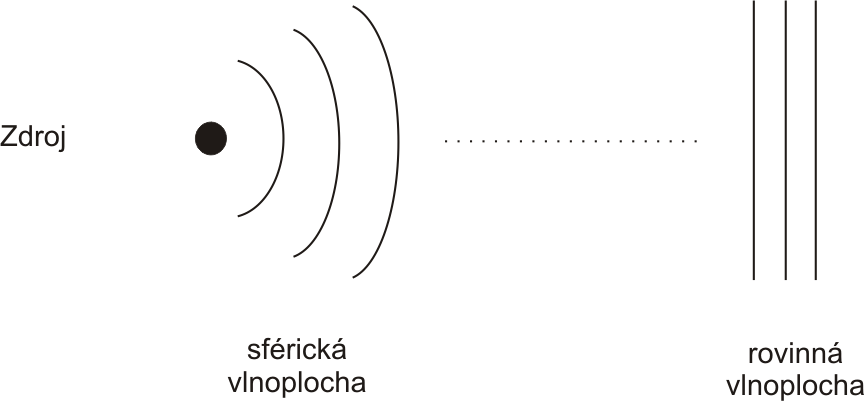
\includegraphics[width=9cm]{evlny_rovinna_vlna.png}
	\caption{Přiblížení rovinné vlny ve vzdáleném prostředí.}
	\label{obr:evlny_rovinna_vlna}
\end{figure}

V~teorii šíření elektromagnetických vln se dle \cite{emp} užívá řada pojmů, z~nichž některé jsou použity také v~této práci.
\begin{itemize}
\item {\bf Vlnoplocha} - Skupina bodů, které mají stejnou fázi a po jejich spojení tvoří geometrickou plochu vlny.
\item {\bf Volné neohraničené prostředí} - Prostor bez jakýkoliv překážek, kterými jsou předměty nebo objekty s~odlišnými materiálovými konstatami  $\varepsilon$, $\mu$ a $\sigma$ od prostředí, ve kterém se vlna šíří.
\item {\bf Homogenní vlna} - Označuje se také jako {\bf uniformní} a jedná se o~vlnu, která má na dané vlnoploše také konstatní amplitudu.
\end{itemize}

Pro analýzu libovolného obecného typu vln je nejprve potřeba zvolit vhodnou souřadnicovou soustavu. V~případě rovinné vlny se bude jednat o~kartézskou souřadnicovou soustavu. V~harmonickém poli bez vnějších zdrojů bude odvození vycházet z~homogenní Helmholtzovy rovnice (\ref{rce:VlnR_ElPole_harm_BezZdroju})
\begin{equation}
	\nabla^{2}\vecfaz E + \faz k^{2}\vecfaz E = 0.
	\label{rce:evlny_VlnR_ElPole_harm_BezZdroju}
\end{equation}
Aplikací operátoru $\nabla^{2}$ na vektor $\vecfaz E$ dostaneme opět vektor, který lze v~kartézské soustavě vyjádřit jako $\nabla^{2}\faz E_{x}\overrightarrow{\mathrm{i}} + \nabla^{2} \faz E_{y}\overrightarrow{\mathrm{j}} + \nabla^{2}\faz E_{z}\overrightarrow{\mathrm{k}}$. To způsobí rozpad vektorové rovnice (\ref{rce:evlny_VlnR_ElPole_harm_BezZdroju}) na skalární rovnice pro jednotlivé složky
\begin{displaymath}
	\nabla^{2} \faz E_{x} +\faz k^{2} \faz E_{x} = 0,
\end{displaymath}
\begin{displaymath}
	\nabla^{2} \faz E_{y} +\faz k^{2} \faz E_{y} = 0,
\end{displaymath}
\begin{displaymath}
	\nabla^{2} \faz E_{z} +\faz k^{2} \faz E_{z} = 0.
\end{displaymath}
Řešení této soustavy rovnic je možné provést {\bf metodou separace proměnných} nebo po zavedení určitých zjednodušujících podmínek jako {\bf jednorozměrnou diferenciální rovnici}, jak je naznačeno dále. Pro vysvětlení druhé varianty se nejprve tyto skalární vztahy rozepíšou následujícím způsobem
\begin{equation}
	\frac{\partial ^{2} \faz E_{x}}{\partial x^{2}} + \frac{\partial ^{2}\faz E_{x}}{\partial y^{2}} + \frac{\partial ^{2}\faz E_{x}}{\partial z^{2}} + \faz k^{2} \faz E_{x} = 0,
	\label{rce:evlny_skalarni1}
\end{equation}
\begin{equation}
	\frac{\partial ^{2} \faz E_{y}}{\partial x^{2}} + \frac{\partial ^{2} \faz E_{y}}{\partial y^{2}} + \frac{\partial ^{2} \faz E_{y}}{\partial z^{2}} + \faz k^{2} \faz E_{y} = 0,
	\label{rce:evlny_skalarni2}
\end{equation}
\begin{equation}
	\frac{\partial ^{2} \faz E_{z}}{\partial x^{2}} + \frac{\partial ^{2} \faz E_{z}}{\partial y^{2}} + \frac{\partial ^{2} \faz E_{z}}{\partial z^{2}} + \faz k^{2} \faz E_{z} = 0.
	\label{rce:evlny_skalarni3}	
\end{equation}
Je výhodné zvolit souřadnicovou soustavu tak, aby se vlna šířila ve směru jedné z~os. Poté bude platit, že vlnoplocha je rovina kolmá na tuto osu, tak jak je naznačeno na obrázku \ref{obr:evlny_vlnoplocha}. Současně uvažujeme pro zjednodušení vektor intenzity elektrického pole pouze ve směru osy $x$. Je možné jej také vyjádřit jako $\vecfaz E = \faz E_{x}\overrightarrow{\mathrm{i}}$.

\begin{figure}[!h]
	\centering
	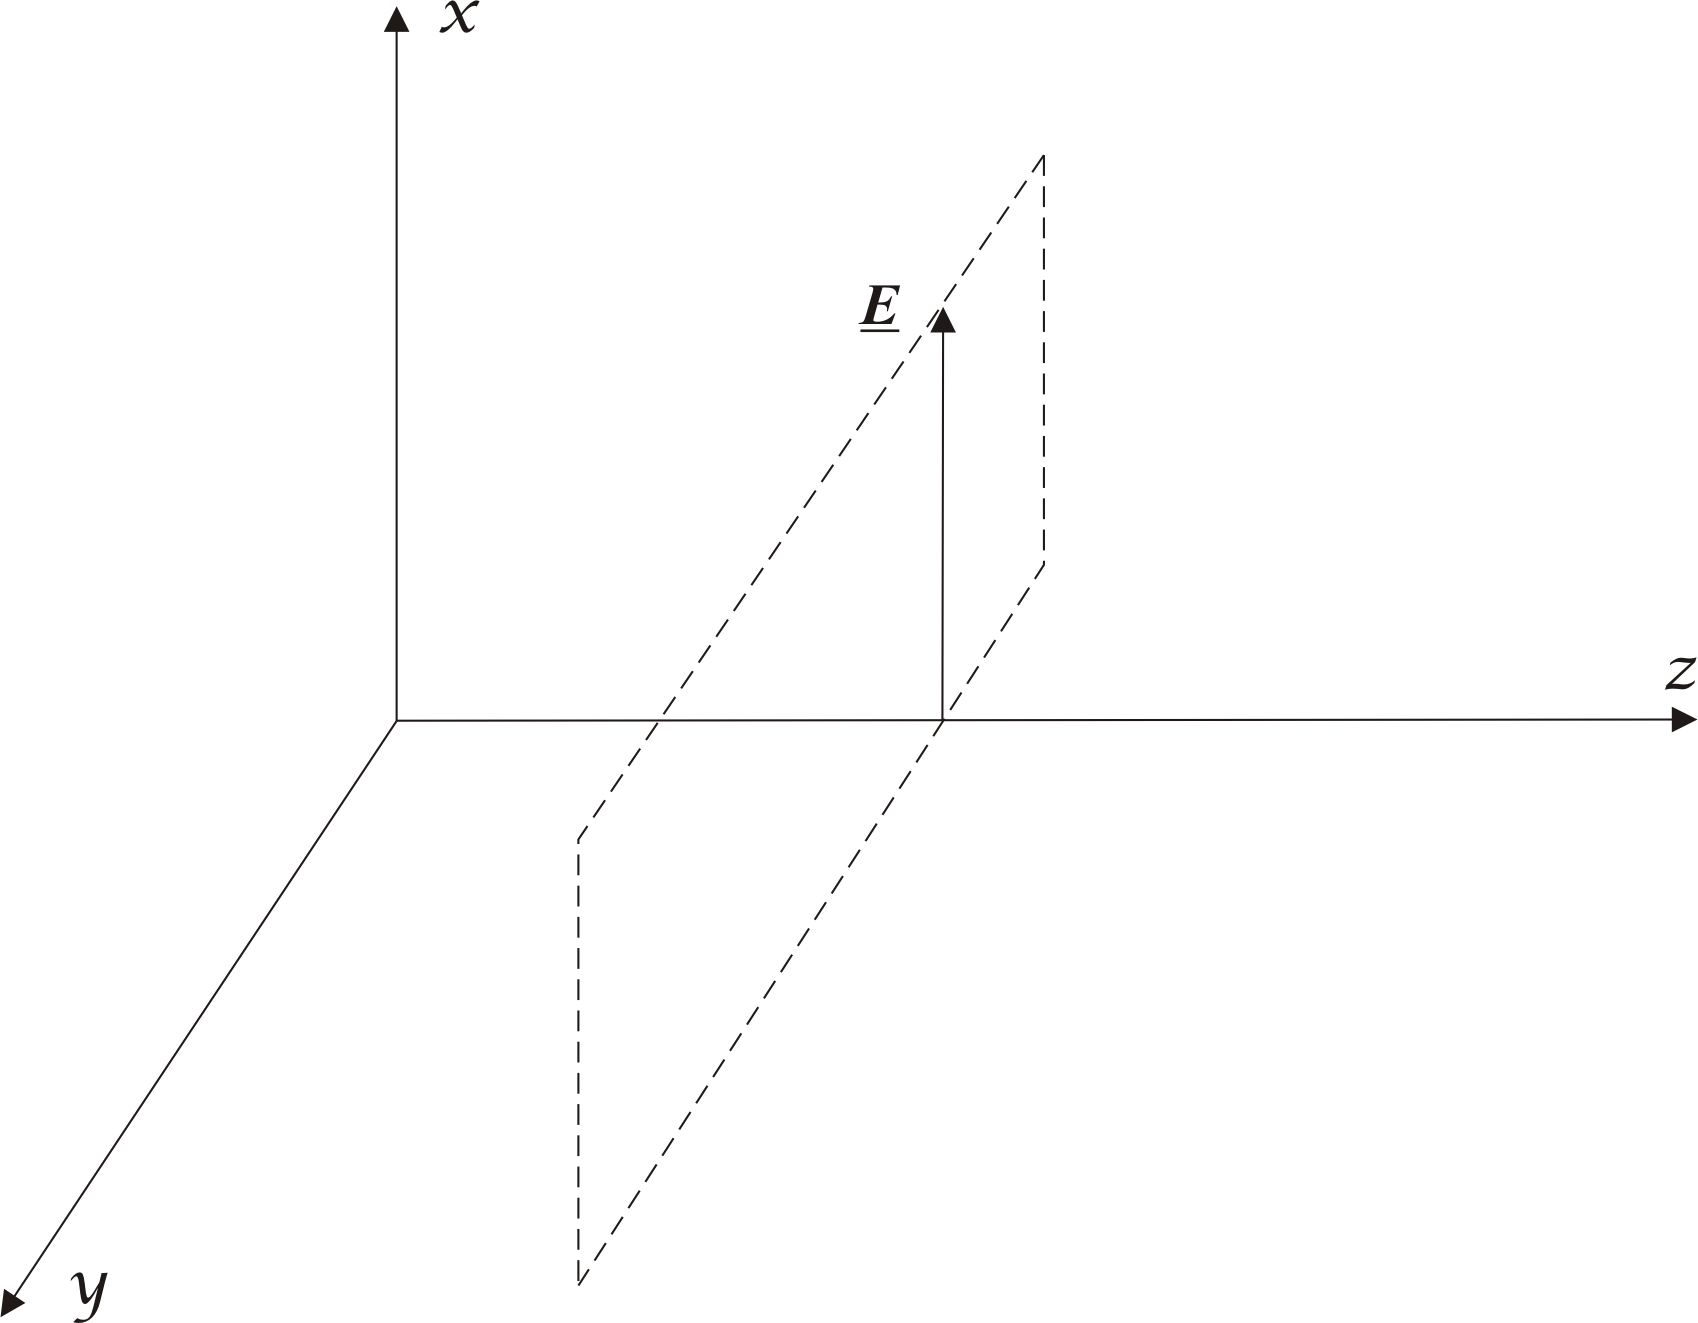
\includegraphics[width=10cm]{evlny_vlnoplocha.png}
	\caption{Vlnoplocha rovinné homogenní vlny. \cite{emp}}
	\label{obr:evlny_vlnoplocha}
\end{figure}

Z~výše uvedených úvah o~charakteru vln a jejich prostorového uspořádání vyplývají následující skutečnosti.
\begin{itemize*}
\item Konstantní velikost a fáze vektoru $\vecfaz E$ ve směru osy $x$, tzn. $\frac{\partial  \faz E_{x}}{\partial x}=0$ a $\frac{\partial \faz E_{x}}{\partial y}=0$.
\item Nulový vektor $\vecfaz E$ ve směru osy $y$, tzn. $ \faz E_{y} = 0$.
\item Nulový vektor $\vecfaz E$ ve směru osy $z$, tzn. $ \faz E_{z} = 0$.
\end{itemize*}
Pokud je aplikujeme na tři rozepsané skalární rovnice (\ref{rce:evlny_skalarni1}) až (\ref{rce:evlny_skalarni3}), dojde ke značnému matematickému zjenodušení. Rovnice (\ref{rce:evlny_skalarni2}) a (\ref{rce:evlny_skalarni3}) se úplně eliminují, u~rovnice (\ref{rce:evlny_skalarni1}) vypadnou první dva členy. Výsledná rovnice bude tak jednorozměrná obyčejná diferenciální druhého řádu ve tvaru
\begin{equation}
	\frac{\partial ^{2} \faz E_{x}}{\partial z^{2}} + \faz k^{2} \faz E_{x} = 0.
	\label{rce:evlny_skalarni}	
\end{equation}

\subsubsection*{Řešení rovnice rovinné homogenní vlny (\ref{rce:evlny_skalarni})}
Vzhledem k~jednoduchosti dané diferenciální rovnice můžeme rovnou předpokládat řešení v~následujícím tvaru
\begin{equation}
	\faz E_{x}(z) = \faz E_{0}^{+}\me^{\lambda_{1}z} +\faz E_{0}^{-}\me^{\lambda_{2}z},
	\label{rce:evlny_reseni1}	
\end{equation}
který představuje superpozici dvou funkcí. Výrazy $E_{0}^{+}$ a $E_{0}^{-}$ jsou komplexní konstanty dané složky vektoru. Parametry $\lambda_{1}$ a $\lambda_{2}$ se určují jako kořeny charakteristického polynomu dané diferenciální rovnice (\ref{rce:evlny_skalarni})
\begin{displaymath}
	\lambda^{2} + \faz k^{2}= 0,
\end{displaymath}
\begin{displaymath}
	\lambda_{1,2} = \pm \sqrt{-\faz k^{2}},
\end{displaymath}
\begin{displaymath}
	\lambda_{1} = -\mj\faz k~,\qquad \lambda_{2} = +\mj\faz k.
\end{displaymath}
Dosazením parametrů $\lambda_{1}$ a $\lambda_{2}$ do (\ref{rce:evlny_reseni1}) dostaneme vztah 
\begin{equation}
	\faz E_{x}(z) = \faz E_{0}^{+}\me^{-\mj\faz k~z} + \faz E_{0}^{-}\me^{\mj\faz k~z},
	\label{rce:evlny_reseni2}	
\end{equation}
který má jednoduchou fyzikální interpretaci. Podle obrázku \ref{obr:evlny_vlnoplocha} je zřejmé, že řešení vlnové rovnice je závislé pouze na souřadnici $z$ a vlnoplocha leží v~rovice $xy$. Takto vyjádřená vlna má pouze jeden stupeň volnosti a může se tedy šířit pouze v~kladném nebo záporném ve směru $z$.

První člen $ \faz E_{0}^{+}\me^{-\mj\faz k z}$ přestavuje funkci vlny šířící se v~kladném směru osy $z$ a označuje se jako {\bf postupná vlna}. Druhý člen $\faz E_{0}^{-}\me^{\mj\faz k z}$ popisuje funkci vlny pohybující se v~opačném směru, tzn. {\bf vlna odražená}.

Komplexní konstanty $\faz E_{0}^{+}$ a $\faz E_{0}^{-}$ je možné dále blíže rozepsat na část představující modul $E_{0\mathrm{mod}}$ a část pro reprezentaci fáze $\me^{j\varphi}$. S~využitím této vlastnosti upravíme rovnici (\ref{rce:evlny_reseni2}). Současně aplikujeme vztah konstanty šíření (\ref{rce:evlny_alphabeta}), tj. $\faz k = \beta - \mj\alpha$,
\begin{displaymath}
	\faz E_{x}(z) = E_{0\mathrm{mod}}^{+}\me^{\mj\varphi^{+}}\me^{-\mj(\beta - \mj\alpha)z} + E_{0\mathrm{mod}}^{-}\me^{\mj\varphi^{-}}\me^{\mj(\beta-\mj\alpha)z}.
\end{displaymath}
Pro určení časové závislosti se nejprve užije vztah (\ref{rce:rotujici_fazor_vektoru}) pro rotující fázor
\begin{displaymath}
	\faz E_{x\,\rot}(z) = E_{0\mathrm{mod}}^{+}\me^{\mj\varphi^{+}}\me^{-\mj\beta z}\me^{-\alpha z}\me^{\mj\omega t} + E_{0\mathrm{mod}}^{-}\me^{\mj\varphi^{-}}\me^{\mj\beta z}\me^{\alpha z}\me^{\mj\omega t}.
\end{displaymath}
Nakonec se podle předpisu (\ref{rce:casova_zavislost}) vyjádří okamžitá hodnota časově proměnné intenzity elektrického pole. Výsledný vztah reprezentuje okamžitou hodnotu postupné a odražené složky rovinné vlny v~harmonickém prostředí
\begin{equation}
	E_{x}(z,t) = E_{0mod}^{+}\me^{-\alpha z}\sin(\omega t - \beta z~+ \varphi^{+}) + E_{0mod}^{-}\me^{\alpha z}\sin(\omega t + \beta z~+ \varphi^{-}).
	\label{rce:evlny_postupna_odrazena}
\end{equation}

\begin{figure}[!h]
	\centering
	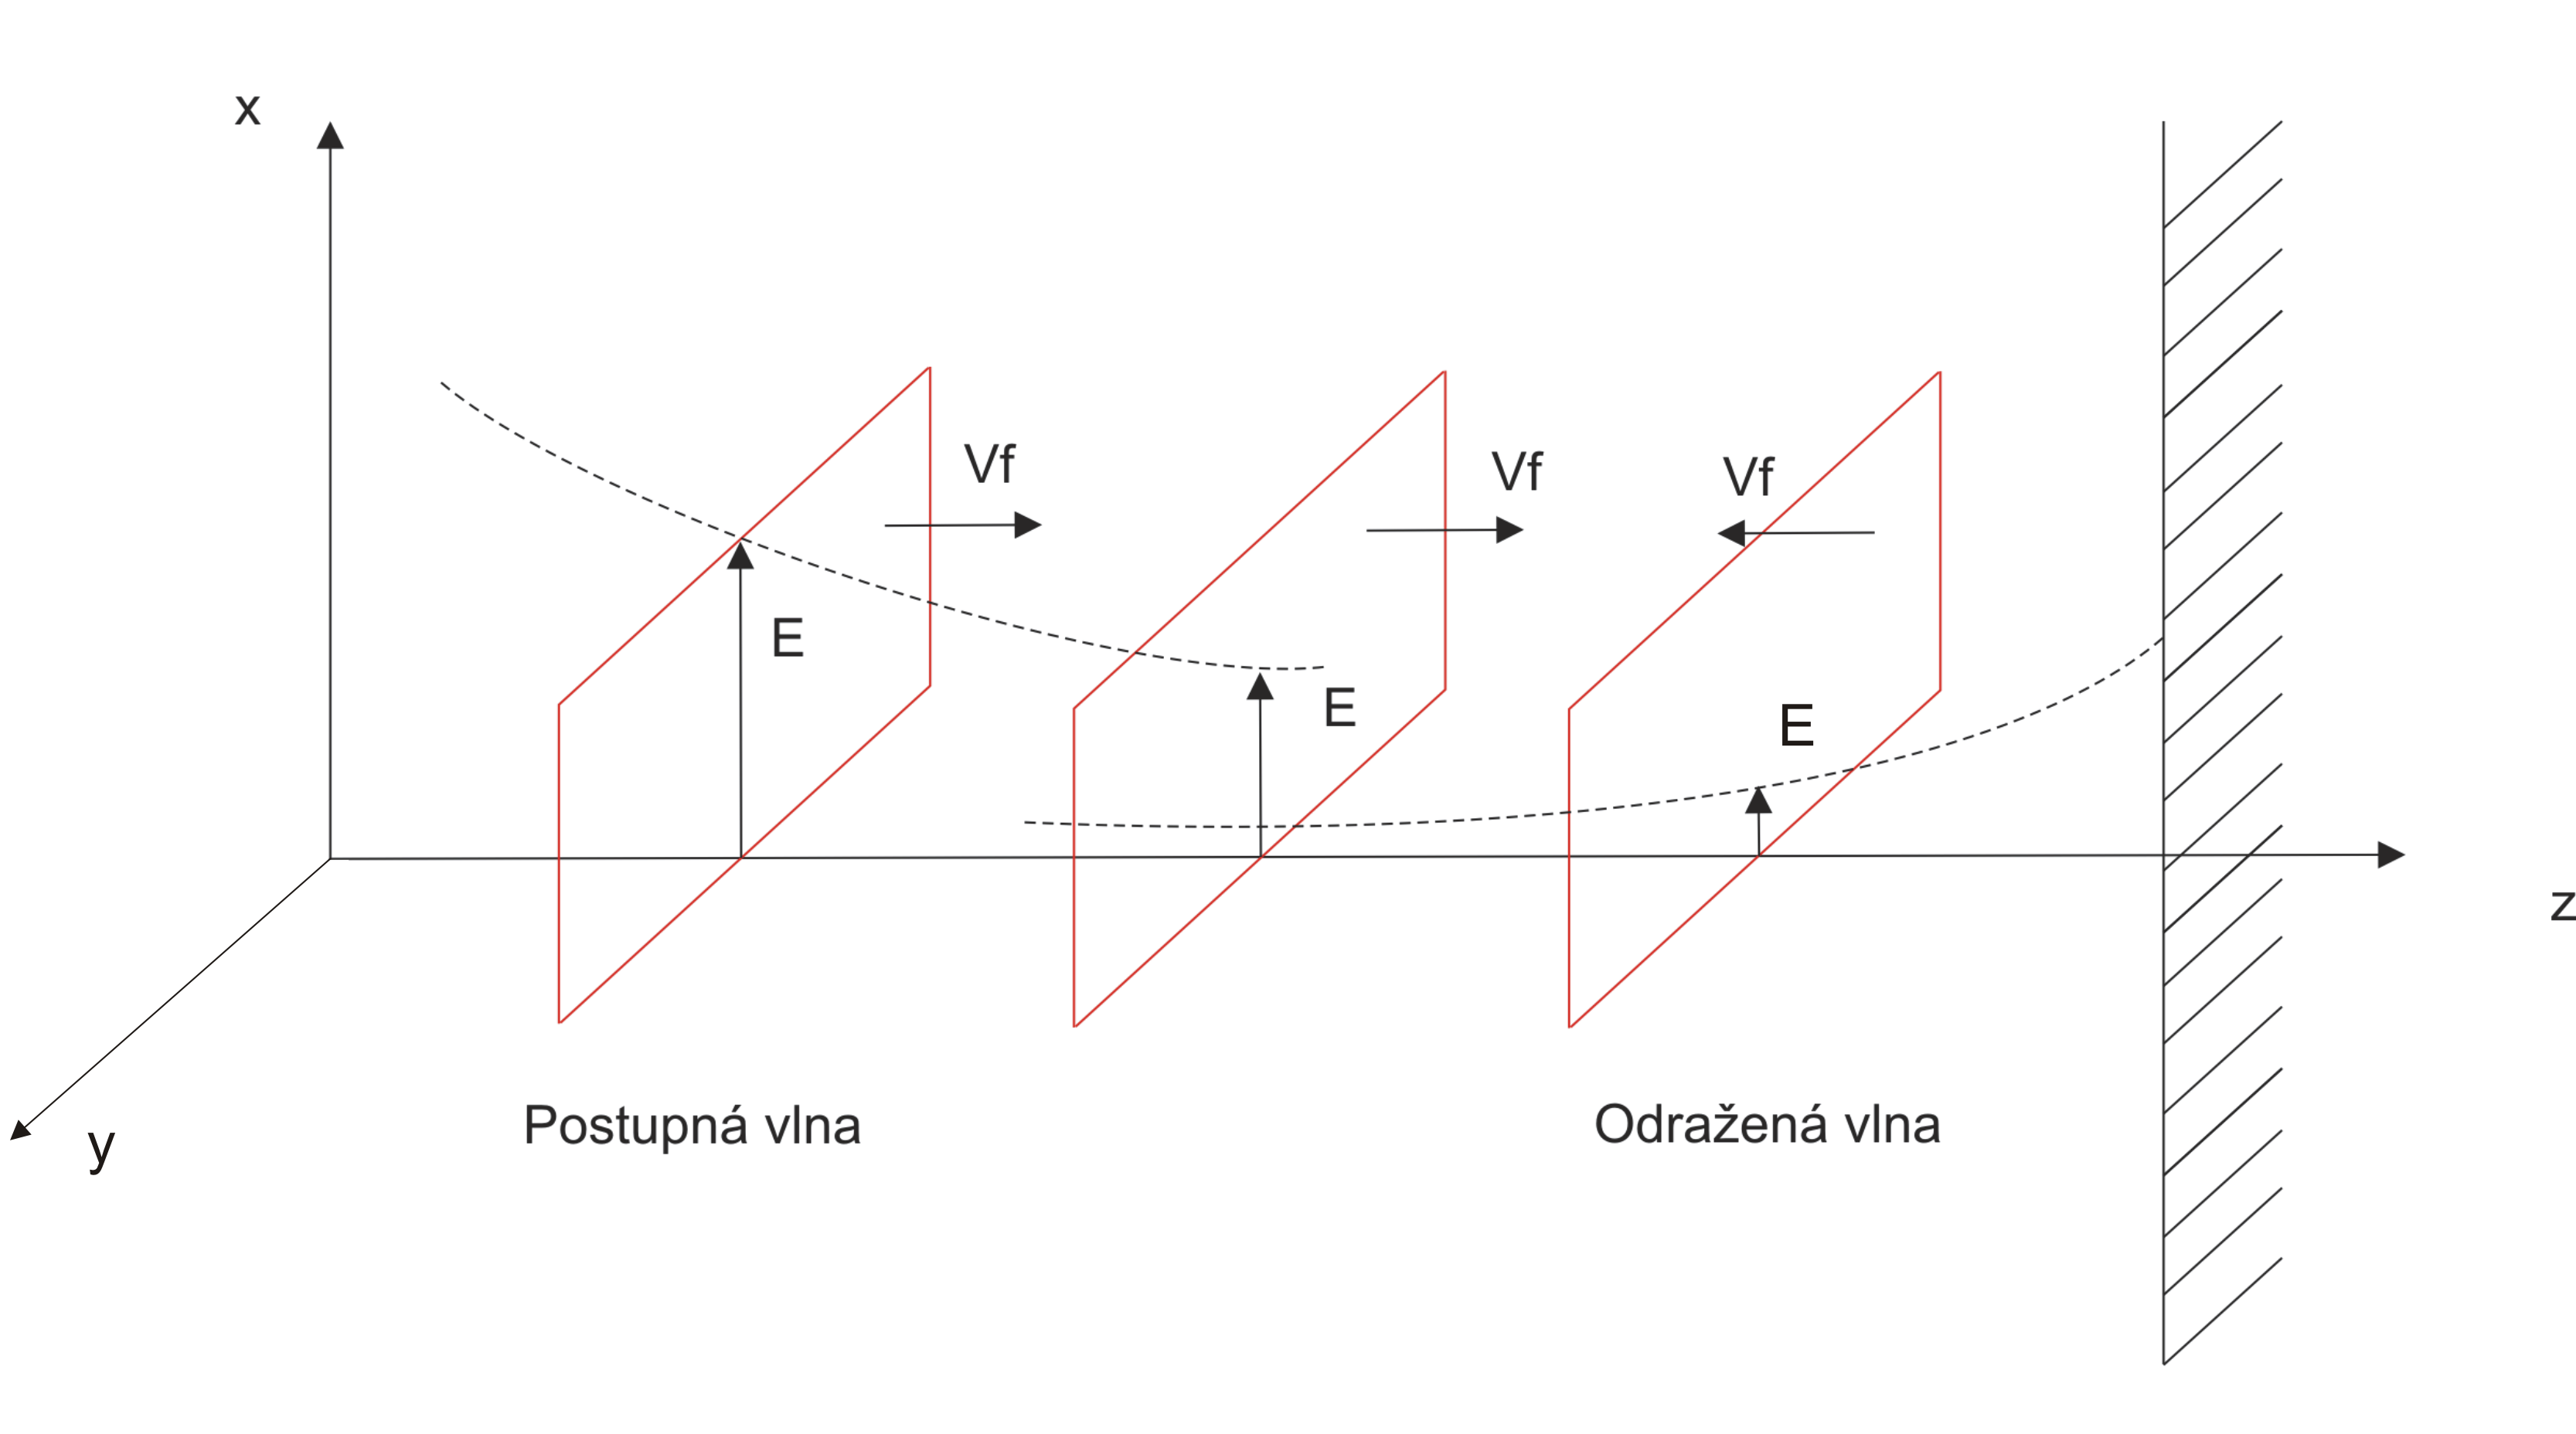
\includegraphics[width=14cm]{evlny_postupna_odrazena.png}
	\caption{Šíření postupné a odražené rovinné vlny fázovou rychlostí $v_f$ dle (\ref{rce:evlny_postupna_odrazena}).}
	\label{obr:evlny_postupna_odrazena}
\end{figure}
\subsubsection*{Fázová rychlost vlny $v_{f}$}
Na obrázku \ref{obr:evlny_postupna_odrazena} je naznačen směr pohybu postupné vlny pomocí $v_{f}$. Rychlost, kterou se vlnoplocha ve směru osy $z$ pohybuje se označuje jako {\bf fázová rychlost vlny}. Výraz pro vyjádření odvodíme z~rovnice (\ref{rce:evlny_postupna_odrazena}). Vzhledem k~tomu, že vlnoplocha představuje rovinu bodů se stejnou fází, bude v~rovnici platit, $\omega t - \beta z + \varphi^{+} = \mathrm{konst.}$ pro postupnou vlnu. Podobně pro odraženou lze zapsat $\omega t + \beta z + \varphi^{-} = \mathrm{konst.}$

Pro odvození fázové rychlosti postupné vlny zderivujeme výraz $\omega t - \beta z + \varphi^{+} = \mathrm{konst.}$ podle času a následně upravíme
\begin{displaymath}
	\omega - \beta \frac{\dif z}{\dif t} = 0,
\end{displaymath}
\begin{displaymath}
	v_{f} = \frac{\dif z}{\dif t} = \frac{\omega}{\beta}\unit{[m/s]}.
\end{displaymath}
Analogickým odvozením z~výrazu pro odraženou vlnu  $\omega t + \beta z + \varphi^{-} = \mathrm{konst.}$ dostaneme vztah, který potvrzuje skutečnost, že odražená vlna se šíří podle osy $z$ v~opačném směru 
\begin{displaymath}
	v_{f} = - \frac{\omega}{\beta}\unit{[m/s]}.
\end{displaymath}

\subsubsection*{Obecné řešení rovnice (\ref{rce:evlny_VlnR_ElPole_harm_BezZdroju}) metodou separace proměnných}
V~řadě aplikacích není možné zavést pro řešení rovnice $\nabla^{2}\vecfaz E +\faz k^{2}\vecfaz E = 0$  zjednodušující předpoklady, vycházející z~obrázku \ref{obr:evlny_vlnoplocha}. Pokud se rovnice neřeší numericky, další analytický postup je možný pomocí metody separace proměnných. Principem je nalézt řešení pro jednotlivé složky vektoru $\vecfaz E$ pomocí součinu tří funkcí, vždy jedné proměnné
\begin{equation}
	\faz E_{i}(x,y,z) = X(x)\cdot Y(y)\cdot Z(z)\qquad\mathrm{pro}\ i = x, y, z.
	\label{rce:evlny_obecne_xyz}
\end{equation}
Podrobné odvození je rozepsáno v~\cite[str. 50]{emp}. Řešení je ve tvaru součinů podle (\ref{rce:evlny_obecne_xyz})
\begin{equation}
	\faz E_{i}(x,y,z) = \big( \faz C_{1}\me^{\mj k_{x}x} +\faz C_{2}\me^{-\mj k_{x}x} \big)\big(\faz C_{3}\me^{\mj k_{y}y} + \faz C_{4}\me^{-\mj k_{y}y} \big)\big(\faz C_{5}\me^{\mj k_{z}z} + \faz C_{6}\me^{-\mj k_{z}z} \big).
	\label{rce:evlny_obecne_reseni}
\end{equation}
Všechny neznámé konstanty se určují na základě okrajových podmínek. Komplexní konstanty $\faz C_{1,\ldots,6}$ udávají amlitudu a fázi rovinných vln, složky konstanty šíření $k_{x}$, $k_{y}$ a $k_{z}$ určují směry šíření. Pomocí součtu určitého množství rovinných vln je tedy možné sestavit v~kartézské souřadnicové soustavě libovolnou vlnu.

\section{Rozhraní dvou prostředí} \label{sec:evlny_rozhrani_dvou_prostredi}
Podkapitola \ref{sec:evlny_volne_prostredi} se věnuje šíření elektromagnetických vln ve volném neohraničeném prostředí. Avšak pro reálnější popis je potřeba zvažovat také vliv překážek v~prostorově omezené oblasti. Důležitým stavebním kamenem pro formulování tohoto problém je, jak napovídá název podkapitoly, chování vln na rozhraní mezi odlišnými prostředími.

Při dopadu elektromagnetické vlny na materiálově odlišný objekt může dojít k~několika událostem, kterými jsou odraz, lom nebo prostup vlny. V~praxi se přirozeně nejedná striktně o~jeden typ chování. Častěji dojde k~jejich kombinaci, ve které mají jednotlivé složky určité zastoupení. Fyzikální vysvětlení spočívá v~existenci vodivých a posuvných proudů, které vzniknou právě při dopadu elektromagnetické vlny. Proudy představují zdroje pro vznik dalších vln, které se superponují k~původní vlně a ovlivní její vlastnosti. 

Matematický popis je možný u~některých příkladů po zavedení určitých zjednodušujících předpokladů. Vytvoření modelu pro obecný reálný případ nemusí být mnohdy vůbec proveditelné, neboť po dopadu vlny na překážku mohou nastat velmi komplikované procesy. Pro názornost je níže vysvětleno o~jaké procesy se může jednat v~jednoduchém případě rovinné homogenní vlny dopadající na rovinné rozhraní.

\subsection*{Chování rovinné vlny na rovinném rozhraní}
Tento případ by se z~hlediska matematického popisu dal nazvat jako téměř ideální. V~reálných variantách bude situace přirozeně jiná, ale i na tomto jednoduchém příkladu je možné popsat jevy, které nastanou po dopadu elektromagnetické vlny. 

Pro popis šíření se výhodně využívá dle \cite[str.47]{emp} tzv. vlnový vektor $\vec k_{vln}$. S~jeho pomocí lze snadno názorně popsat směry šíření vln na rozhraní. Vlnový vektor představuje to, v~jakém směru se šíří vlnoplocha. Dle obrázku \ref{obr:evlny_vlnovy_vektor} jej lze pomocí konstanty šíření $\faz k$ definovat
\begin{equation}
	\vec k_{vln} = \faz k~\vec n_{0} = k_{x}\overrightarrow{\mathrm{i}} + k_{y}\overrightarrow{\mathrm{j}} + k_{z}\overrightarrow{\mathrm{k}}.
	\label{rce:evlny_vlnovy_vektor}
\end{equation}

\begin{figure}[!h]
	\centering
	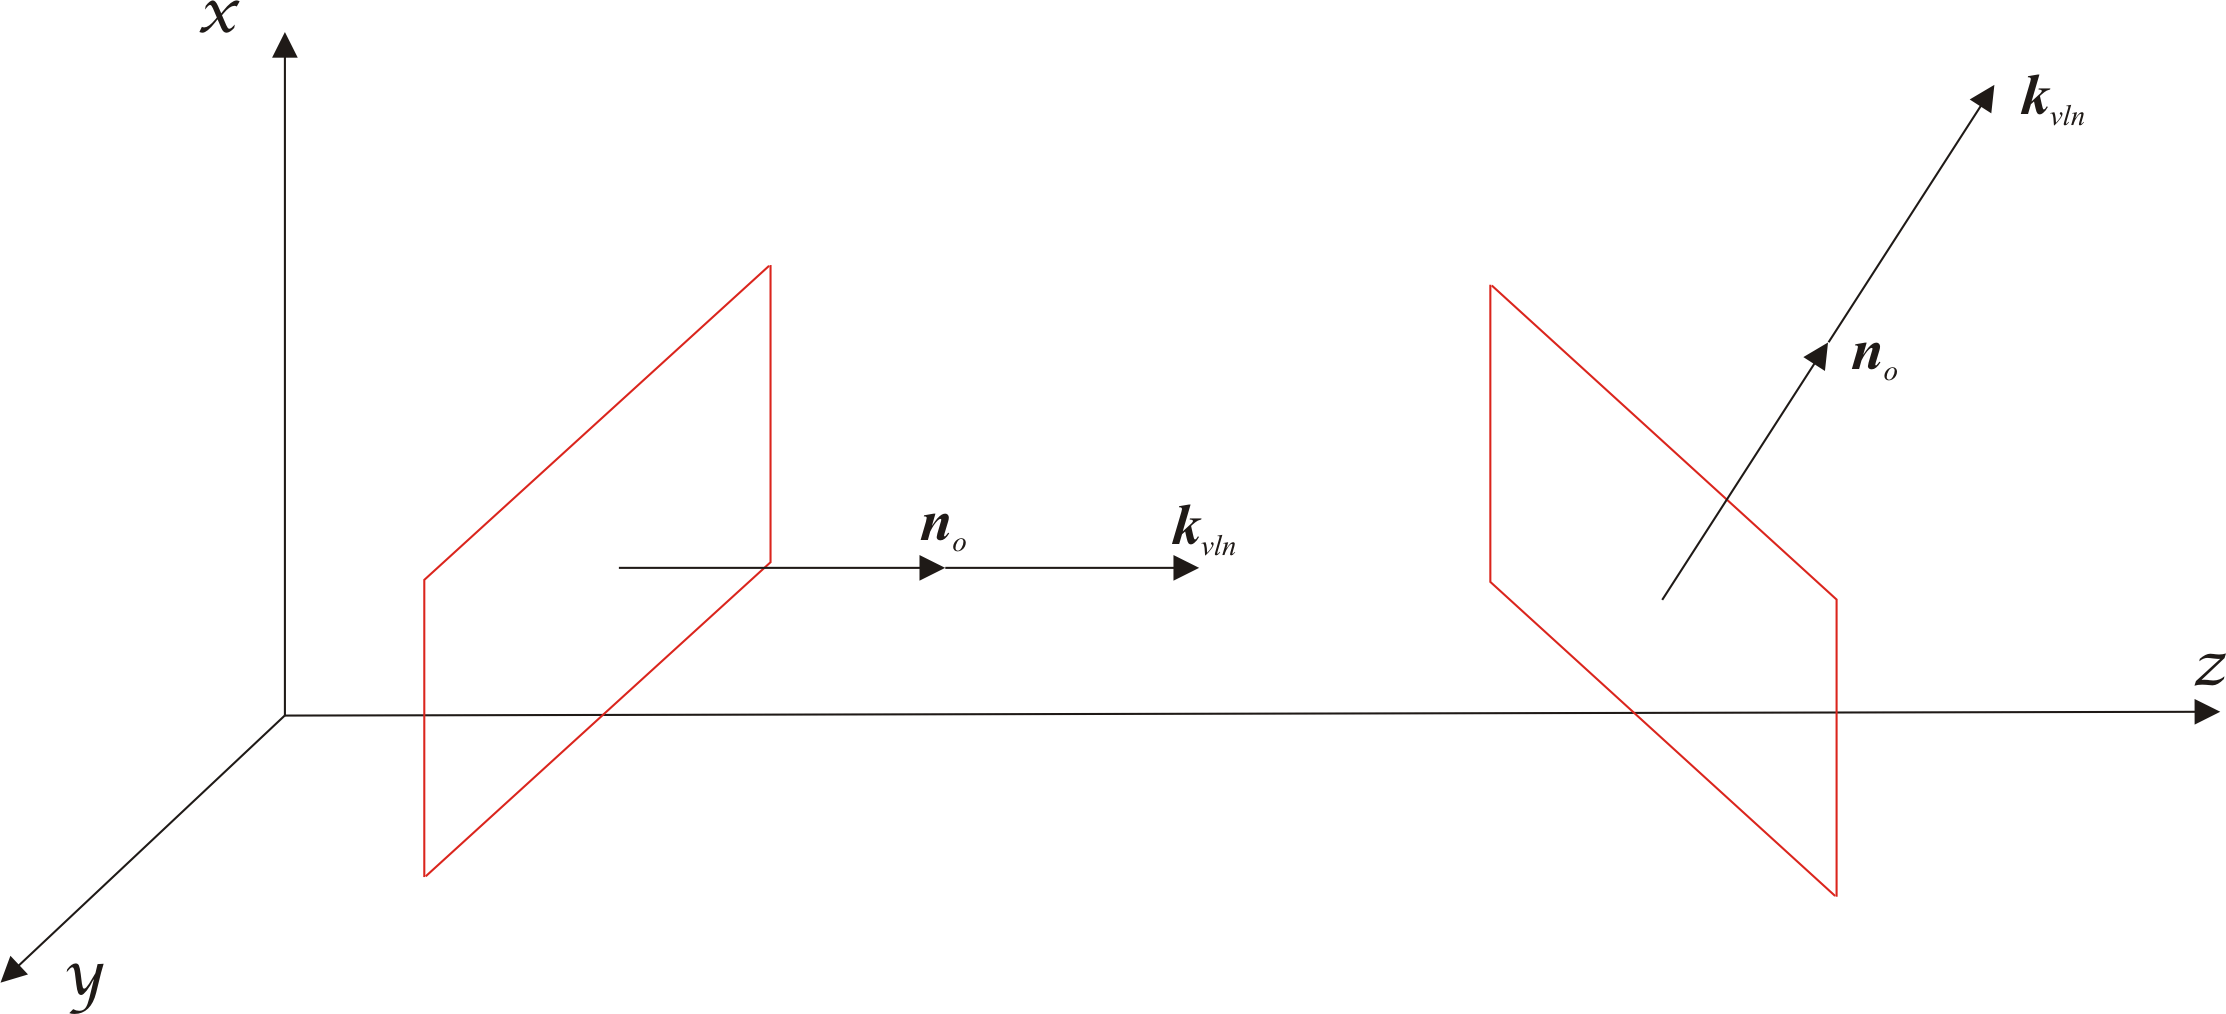
\includegraphics[width=13cm]{evlny_vlnovy_vektor.png}
	\caption{Definice vlnového vektoru v~kartézské soustavě souřadnic. \cite{emp}}
	\label{obr:evlny_vlnovy_vektor}
\end{figure}

Podle naznačené situace na obrázku \ref{obr:evlny_rovinne_rozhrani} je zřejmé, jak se může zachovat elektromagnetická vlna při dopadu pod obecným úhlem na rovinné rozhraní. Může dojít k~odrazu od rozhraní nebo průchodu do sousedícího prostředí, přičemž se se změní směr šíření (dojde k~lomu). Nejčastější bude případ, kdy se část vlny odrazí a současně část projde a bude se lámat. 

\begin{figure}[!h]
	\centering
	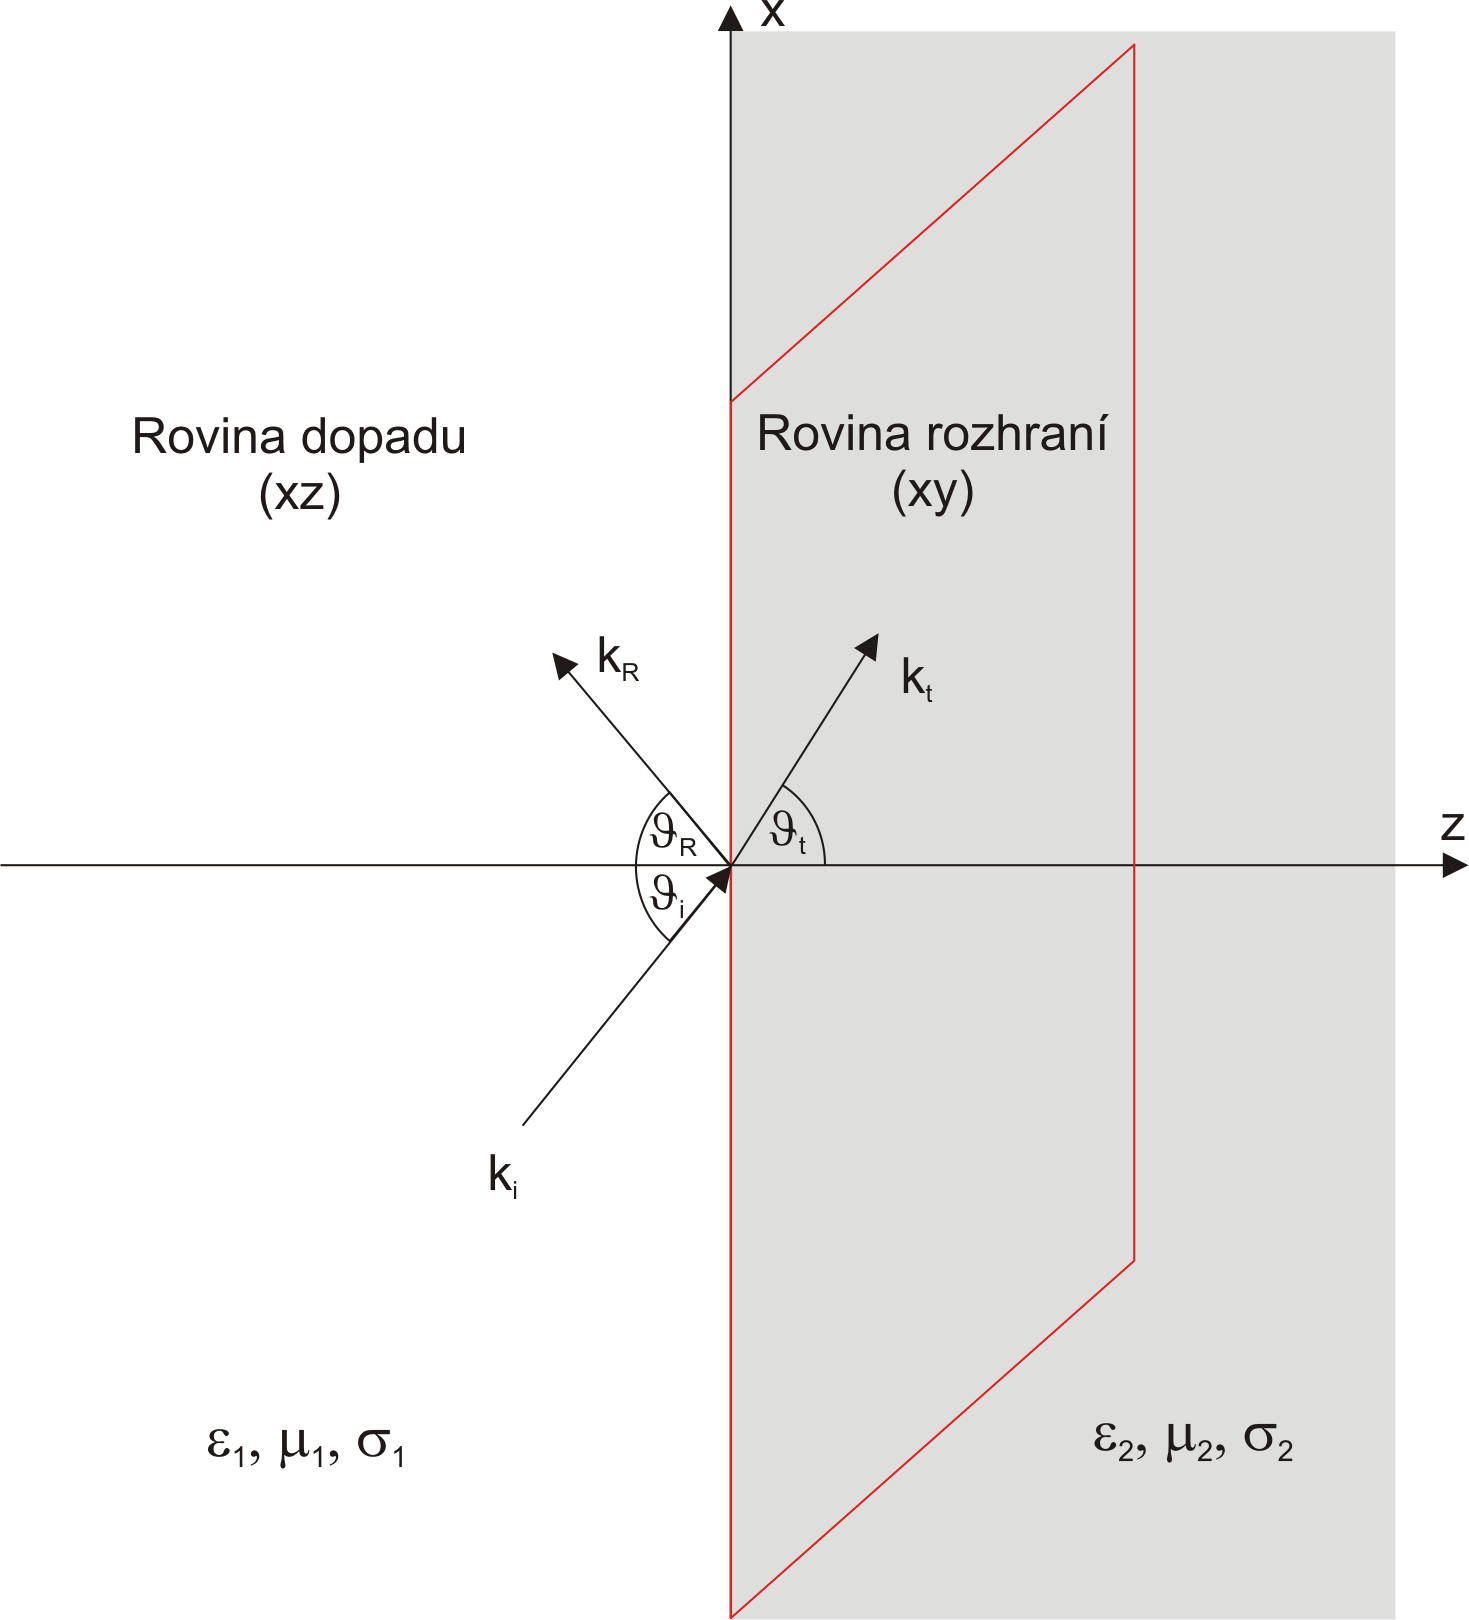
\includegraphics[width=8cm]{evlny_rovinne_rozhrani.png}
	\caption{Obecný dopad rovinné vlny na rozhraní s~využitím vlnového vektoru.}
	\label{obr:evlny_rovinne_rozhrani}
\end{figure}

Jak je navíc z~obrázku patrné, hranice mezi prostředími leží v~rovině $xy$. Označuje se jako {\bf rovina rozhraní}. Jednotlivé prostředí se liší materiálovými konstantami $\varepsilon$, $\mu$ a $\sigma$. Vlna se šíří ve směru osy $z$, tak jak bylo uvažováno již v~podkapitole \ref{sec:evlny_volne_prostredi}. Dopadá na rovinu rozhraní pod úhlem $\vartheta_{i}$ (z~anglického \uv{incident wave}). Část vlny se odráží pod úhlem $\vartheta_{r}$ (\uv{ref{l}ected}) a část proniká pod úhlem $\vartheta_{t}$ (\uv{transmitted}). Vlnové vektory všech tří variant jsou vyznačeny na obrázku \ref{obr:evlny_rovinne_rozhrani}. Rovina, ve které leží vektor dopadající vlny $k_{i}$, tvořená osami $xz$, se značí jako {\bf rovina dopadu}.

Splnění podmínek na rozhraní pro tečné složky vektorů $\vec E$ a $\vec H$ nastane, když jsou shodné $x$-ové složky vlnových vektorů, tj. $k_{i\,x} = k_{r\,x} = k_{t\,x}$. Dle obrázku \ref{obr:evlny_rovinne_rozhrani} je patrné, že s~využitím naznačených úhlů, lze zapsat
\begin{displaymath}
	\vec k_{i}\sin\vartheta_{i} = \vec k_{r}\sin\vartheta_{r} = \vec k_{t}\sin\vartheta_{t}.
\end{displaymath}
Vzhledem k~shodnosti prostředí, ve kterém se nachází postupná a odražená vlna, je možné s~využitím vztahu (\ref{rce:evlny_vlnovy_vektor}) definovat $\faz k_{1}\vec n_0 = \vec k_{i} = \vec k_{r}$. Obdobně pro druhé prostředí platí $\faz k_{2}\vec n_0 = \vec k_{t}$. Vyjádřený vztah (\ref{rce:evlny_snell_odvozeni}) je výchozím pro Snellovy zákony
\begin{equation}
	\faz k_{1}\sin\vartheta_{i} = \faz k_{1}\sin\vartheta_{r} = \faz k_{2}\sin\vartheta_{t}.
	\label{rce:evlny_snell_odvozeni}
\end{equation}
\begin{itemize}
\item {\bf Zákon odrazu} - Platí pro dopadající a odraženou elektromagnetickou vlnu. Lze jej také ústně interpretovat jako: \uv{Úhel odrazu se rovná úhlu dopadu}
\end{itemize}
\begin{displaymath}
	\faz k_{1}\sin\vartheta_{i} = \faz k_{1}\sin\vartheta_{r},
\end{displaymath}
\begin{equation}
	\vartheta_{i} = \vartheta_{r}.
	\label{rce:evlny_zakon_odrazu}
\end{equation}
\begin{itemize}
\item {\bf Zákon lomu} - Platí pro dopadající vlnu a pro vlnu pronikající do druhého prostředí
\end{itemize}
\begin{displaymath}
	\faz k_{1}\sin\vartheta_{i} = \faz k_{2}\sin\vartheta_{t},
\end{displaymath}
\begin{equation}
	\frac{\faz k_{2}}{\faz k_{1}} = \frac{\sin\vartheta_{i}}{\sin\vartheta_{t}}.
	\label{rce:evlny_zakon_lomu}
\end{equation}

\subsection{Kolmý dopad rovinné vlny na rozhraní} \label{subsec:kolmy_dopad}
V~konkrétním případě, dle obrázku \ref{obr:evlny_dielektricke_rozhrani}, je naznačen dopad rovinné homogenní vlny na rovinné rozhraní mezi dvěma prostředími. Ty jsou popsány obecně materiálovými parametry $\varepsilon_{1,2}$, $\mu_{1,2}$ a $\sigma_{1,2}$. Z~nich je možné vztahem $\faz Z=\sqrt{\frac{\mj\omega\mu}{\mj\omega\varepsilon + \sigma}}$ vyjádřit vlnové impedance pro jednotlivé prostředí.

\begin{figure}[!h]
	\centering
	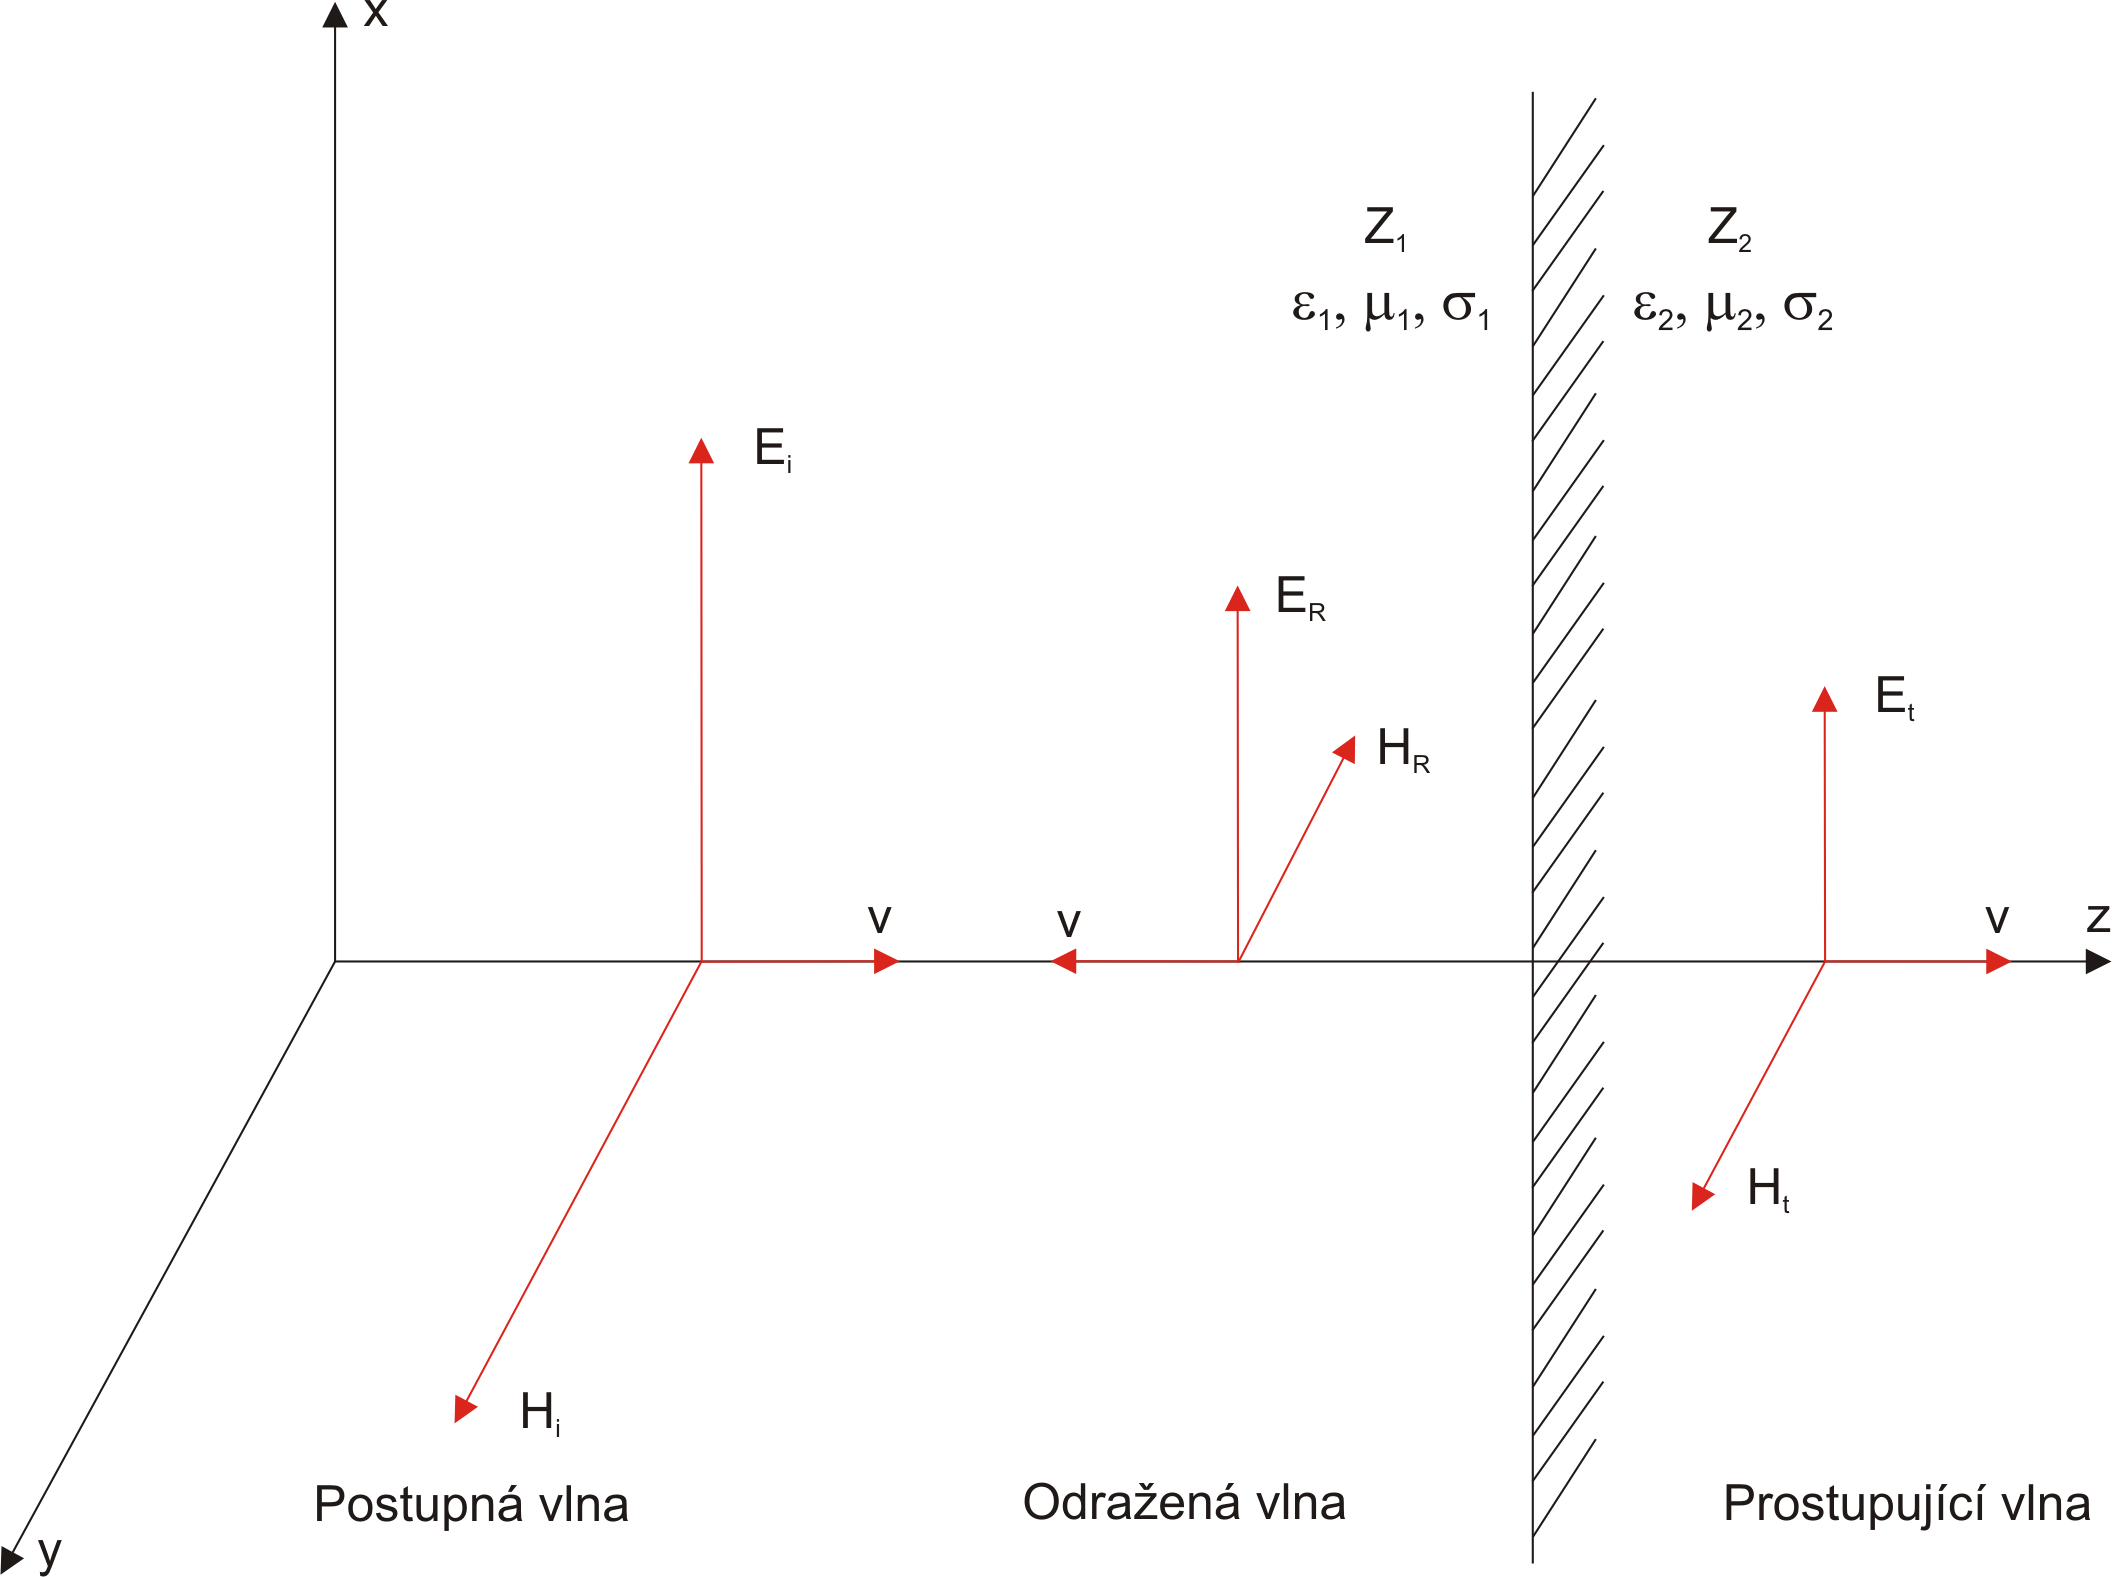
\includegraphics[width=13.5cm]{evlny_dielektricke_rozhrani.png}
	\caption{Kolmý dopad rovinné vlny rozhraní mezi dielektriky.}
	\label{obr:evlny_dielektricke_rozhrani}
\end{figure}

Vlny, které dopadají na rozhraní, lze zapsat vztahy pro vektory intezity elektrického pole $\vecfaz E_{i}$ a magnetického $\vecfaz H_{i}$ v~závislosti na souřadnici $z$
\begin{displaymath}
	\vecfaz E_{i}(z) = \faz E_{i0}\me^{-\mj\faz k_{1}z}\overrightarrow{\mathrm{i}},
\end{displaymath}
\begin{displaymath}
	\vecfaz H_{i}(z) = \frac{\faz E_{i0}}{\faz Z_{1}}\me^{-\mj\faz k_{1}z}\overrightarrow{\mathrm{j}}.
\end{displaymath}
Pro odraženou vlnu platí
\begin{displaymath}
	\vecfaz E_{r}(z) = \faz E_{r0}\me^{\mj\faz k_{1}z}\overrightarrow{\mathrm{i}},
\end{displaymath}
\begin{displaymath}
	\vecfaz H_{r}(z) = - \frac{\faz E_{r0}}{\faz Z_{1}}\me^{\mj\faz k_{1}z}\overrightarrow{\mathrm{j}},
\end{displaymath}
a~nakonec pro prostupující vlnu
\begin{displaymath}
	\vecfaz E_{t}(z) = \faz E_{t0}\me^{-\mj\faz k_{2}z}\overrightarrow{\mathrm{i}},
\end{displaymath}
\begin{displaymath}
	\vecfaz H_{t}(z) = \frac{\faz E_{t0}}{\faz Z_{2}}\me^{-\mj\faz k_{2}z}\overrightarrow{\mathrm{j}}.
\end{displaymath}
Podle podmínek na rozhraní ($z = 0$) se určí závislosti komplexních amplitud. Vychází se z~uvedených vztahů pro dopadající, odraženou a pronikající vlnu.
Pro vektor intenzity elektrického pole platí
\begin{displaymath}
	\vecfaz E_{i}(0) + \vecfaz E_{r}(0)  = \vecfaz E_{t}(0),
\end{displaymath}
\begin{displaymath}
	 \faz E_{i0}\me^{-j\faz k_{1}0}\overrightarrow{\vec{i}} + \faz E_{r0}\me^{j\faz k_{1}0}\overrightarrow{\mathrm{i}}  = \faz E_{t0}\me^{-j\faz k_{2}0}\overrightarrow{\mathrm{i}},
\end{displaymath}
\begin{equation}
	\faz E_{i0} + \faz E_{r0}  = \faz E_{t0}.
	\label{rce:evlny_rozhrani_E}
\end{equation}
Pro vektor intenzity magnetického pole na daném rozhraní se jedná o~analogické odvození, tj. $\vecfaz H_{i}(0) + \vecfaz H_{r}(0)  = \vecfaz H_{t}(0)$, čímž dostaneme
\begin{equation}
	\frac{\faz E_{i0}-\faz E_{r0}}{\faz Z_{1}} = \frac{\faz E_{t0}}{\faz Z_{2}}.
	\label{rce:evlny_rozhrani_H}
\end{equation}
Za $\faz E_{t0}$ se dosadí z~rovnice (\ref{rce:evlny_rozhrani_E}) do (\ref{rce:evlny_rozhrani_H}) . Dostaneme závislost $\faz E_{r0}$ na $\faz E_{i0}$, na jejíž základě se dle \cite{emp} definuje {\bf činitel odrazu (reflexe)}  $\faz R = \frac{\faz E_{r0}}{\faz E_{i0}}\unit{[-]}$
\begin{displaymath}
	\frac{\faz E_{i0}-\faz E_{r0}}{\faz Z_{1}} = \frac{\faz E_{i0} + \faz E_{r0}}{\faz Z_{2}},
\end{displaymath}
\begin{displaymath}
	\faz E_{r0}\Big( \frac{1}{\faz Z_{1}} + \frac{1}{\faz Z_{2}} \Big) = \faz E_{i0}\Big( \frac{1}{\faz Z_{1}} - \frac{1}{\faz Z_{2}} \Big),
\end{displaymath}
\begin{equation}
	\faz E_{r0} = \faz E_{i0} \frac{\faz Z_{2}-\faz Z_{1}}{\faz Z_{1}+\faz Z_{2}}.
	\label{rce:evlny_cin_odrazu_odvozeni}
\end{equation}
Z~rovnice (\ref{rce:evlny_cin_odrazu_odvozeni}) je patrný činitel odrazu
\begin{equation}
	\faz R = \frac{\faz Z_{2}-\faz Z_{1}}{\faz Z_{1}+\faz Z_{2}}.
	\label{rce:evlny_cin_odrazu}
\end{equation}
 Pokud chceme vyjádřit závislost $\faz E_{t0}$ na $\faz E_{i0}$ dosadíme z~(\ref{rce:evlny_rozhrani_E}) do (\ref{rce:evlny_rozhrani_H}) za $\faz E_{r0}$. Následně se určuje {\bf činitel prostupu (transmise)}  $\faz T = \frac{\faz E_{t0}}{\faz E_{i0}}\unit{[-]}$ 
\begin{displaymath}
	\frac{\faz E_{i0}-\faz E_{t0}+\faz E_{i0}}{\faz Z_{1}} = \frac{\faz E_{t0}}{\faz Z_{2}},
\end{displaymath}
\begin{displaymath}
	\faz E_{t0} \frac{\faz Z_{1}+\faz Z_{2}}{\faz Z_{1}\faz Z_{2}} = \faz E_{i0} \frac{2}{\faz Z_{1}}.
\end{displaymath}
\begin{equation}
	\faz E_{t0} = \faz E_{i0} \frac{2\faz Z_{2}}{\faz Z_{1}+\faz Z_{2}}.
	\label{rce:evlny_cin_prostupu_odvozeni}
\end{equation}
V~(\ref{rce:evlny_cin_prostupu_odvozeni}) je opět zřejmý činitel prostupu
\begin{equation}
	\faz T = \frac{2\faz Z_{2}}{\faz Z_{1}+\faz Z_{2}}.
	\label{rce:evlny_cin_prostupu}
\end{equation}
Vztahy pro oba činitele (\ref{rce:evlny_cin_prostupu}) a (\ref{rce:evlny_cin_odrazu}) jsou na sobě závislé a řídí se vztahem $1 + \faz R = \faz T$.

\subsection{Dopad rovinné vlny pod obecným úhlem}
Při analýze chování dopadající rovinné vlny pod jiným úhlem, než aby se jednalo o~kolmý dopad, se rozlišuje, zda se jedná o~kolmou (horizontální) nebo rovnoběžnou (vertikální) polarizaci vlny. Orientace se určuje podle vektoru intenzity elektrického pole $\vecfaz E$.
\subsubsection*{Kolmá polarizace}
Vektor $\vecfaz E$ je v~tomto případě kolmý na rovinu dopadu, tj. $xz$, podle obrázku \ref{obr:evlny_kolma_polarizace}.
\begin{figure}[!h]
	\centering
	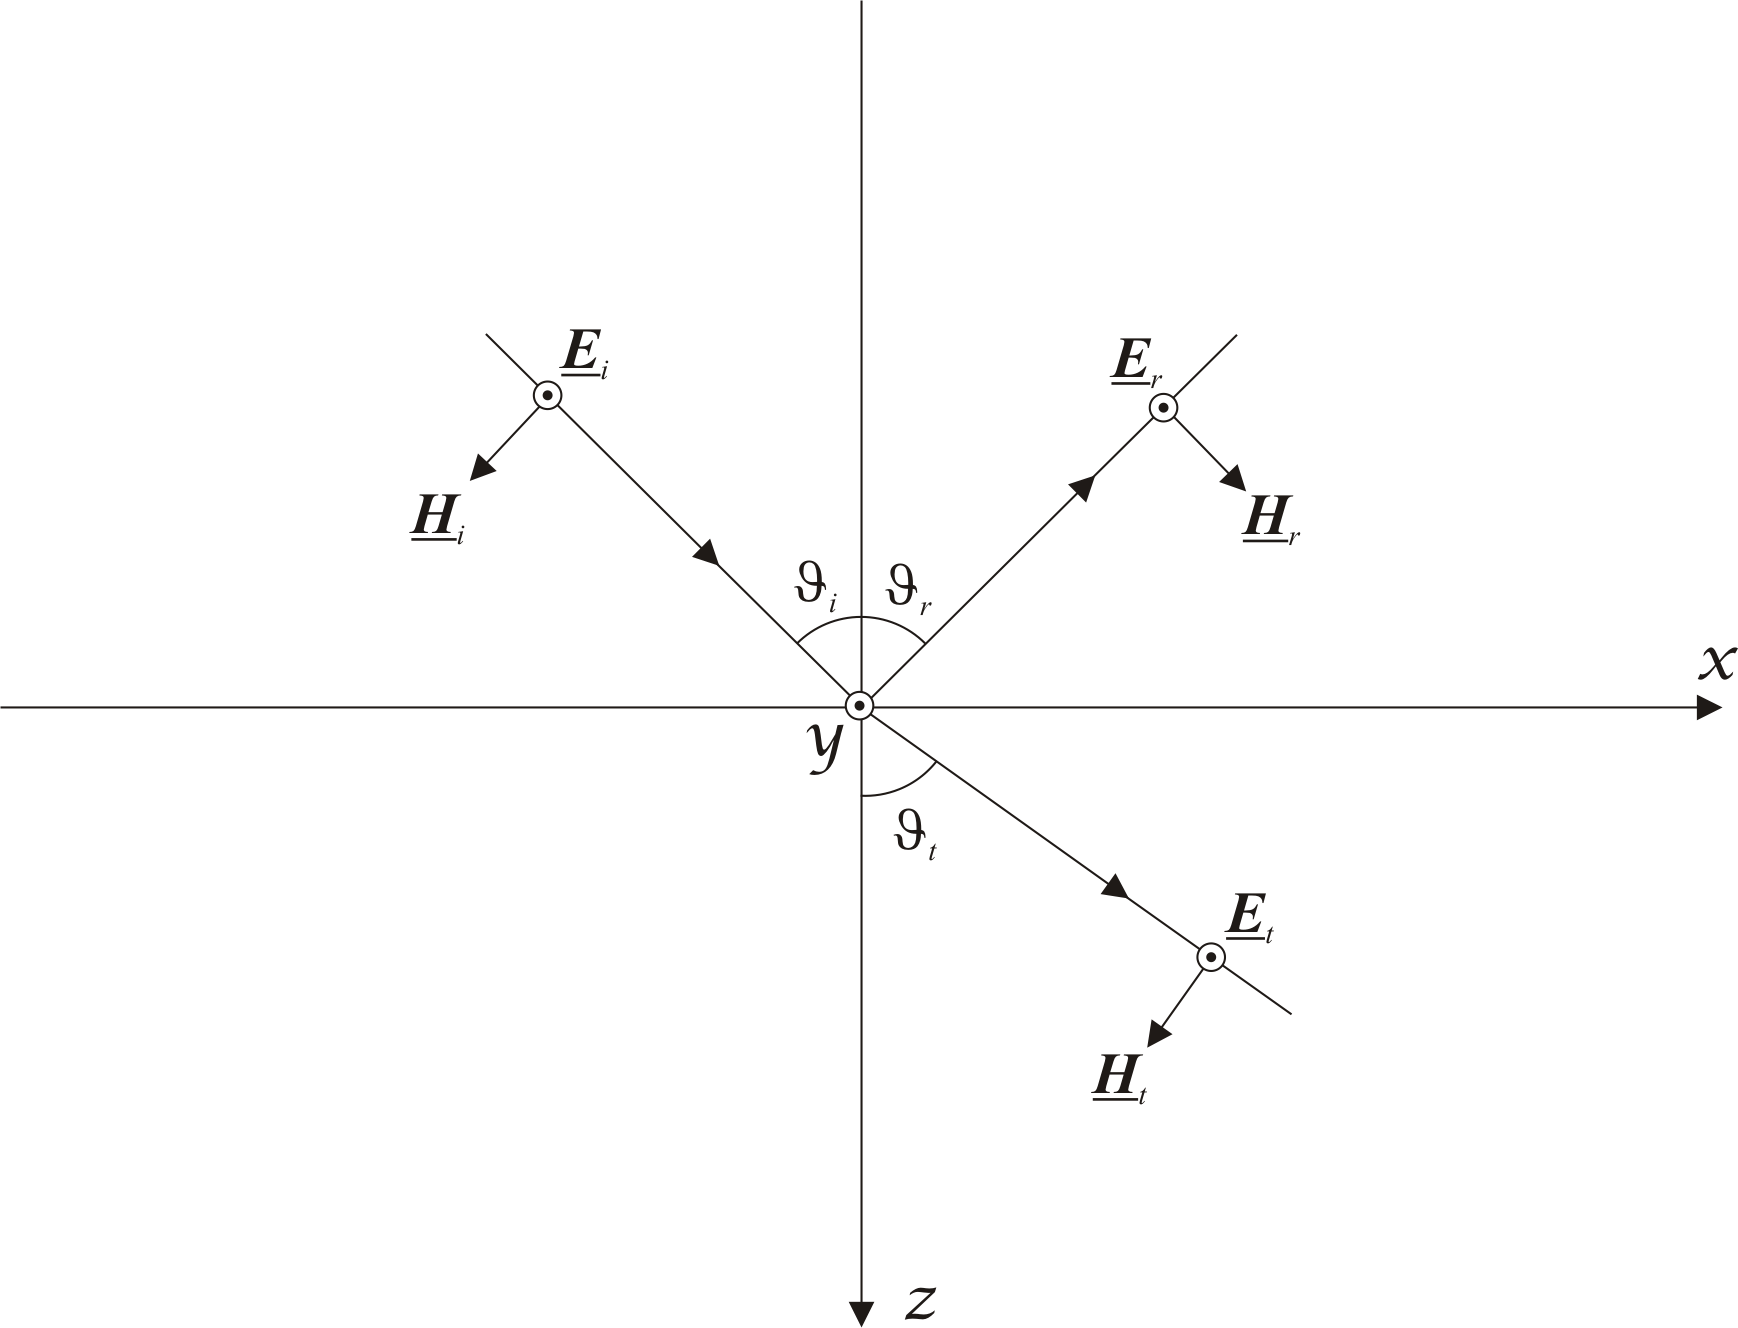
\includegraphics[width=11cm]{evlny_kolma_polarizace.png}
	\caption{Kolmá polarizace rovinné vlny. \cite{emp}}
	\label{obr:evlny_kolma_polarizace}
\end{figure}
Podobně jako v~části \ref{subsec:kolmy_dopad} se také u~této varianty uspořádání definují činitelé odrazu $\faz R_{\perp}$ a prostupu $\faz T_{\perp}$. Analogickým způsobem bychom dostali vztahy, které jsou blíže odvozené v~\cite[str. 94]{emp} a pro které obdobně platí $\faz R_{\perp} + 1 = \faz T_{\perp}$
\begin{equation}
	\faz R_{\perp} = \frac{\faz E_{r0}}{\faz E_{i0}} = \frac{\faz Z_{2}\cos\vartheta_{i}-\faz Z_{1}\cos\vartheta_{t}}{\faz Z_{2}\cos\vartheta_{i}+\faz Z_{1}\cos\vartheta_{t}} = \frac{\faz Z_{2}\cos\vartheta_{i}-\faz Z_{1}\sqrt{1-(\faz k_{1}/\faz k_{2})^{2}\sin^{2}\vartheta_{i}}}{\faz Z_{2}cos\vartheta_{i}+\faz Z_{1}\sqrt{1-(\faz k_{1}/\faz k_{2})^{2}\sin^{2}\vartheta_{i}}},
	\label{rce:evlny_cin_odrazu_kolma}
\end{equation}
\begin{equation}
	\faz T_{\perp} = \frac{\faz E_{t0}}{\faz E_{i0}} = \frac{2\faz Z_{2}\cos\vartheta_{i}}{\faz Z_{2}\cos\vartheta_{i}+\faz Z_{1}\cos\vartheta_{t}} = \frac{2\faz Z_{2}\cos\vartheta_{i}}{\faz Z_{2}\cos\vartheta_{i}+\faz Z_{1}\sqrt{1-(\faz k_{1}/\faz k_{2})^{2}\sin^{2}\vartheta_{i}}}.
	\label{rce:evlny_cin_prostupu_kolma}
\end{equation}

\subsubsection*{Rovnoběžná polarizace}
Pro vektor intenzity elektrického pole platí, že je tentokrát rovnoběžný s~rovinou dopadu $xz$. Současně je vektor $\vecfaz H$ tečný k~rovině rozhraní $xy$, viz. obrázek \ref{obr:evlny_rovnobezna_polarizace}.
\begin{figure}[!h]
	\centering
	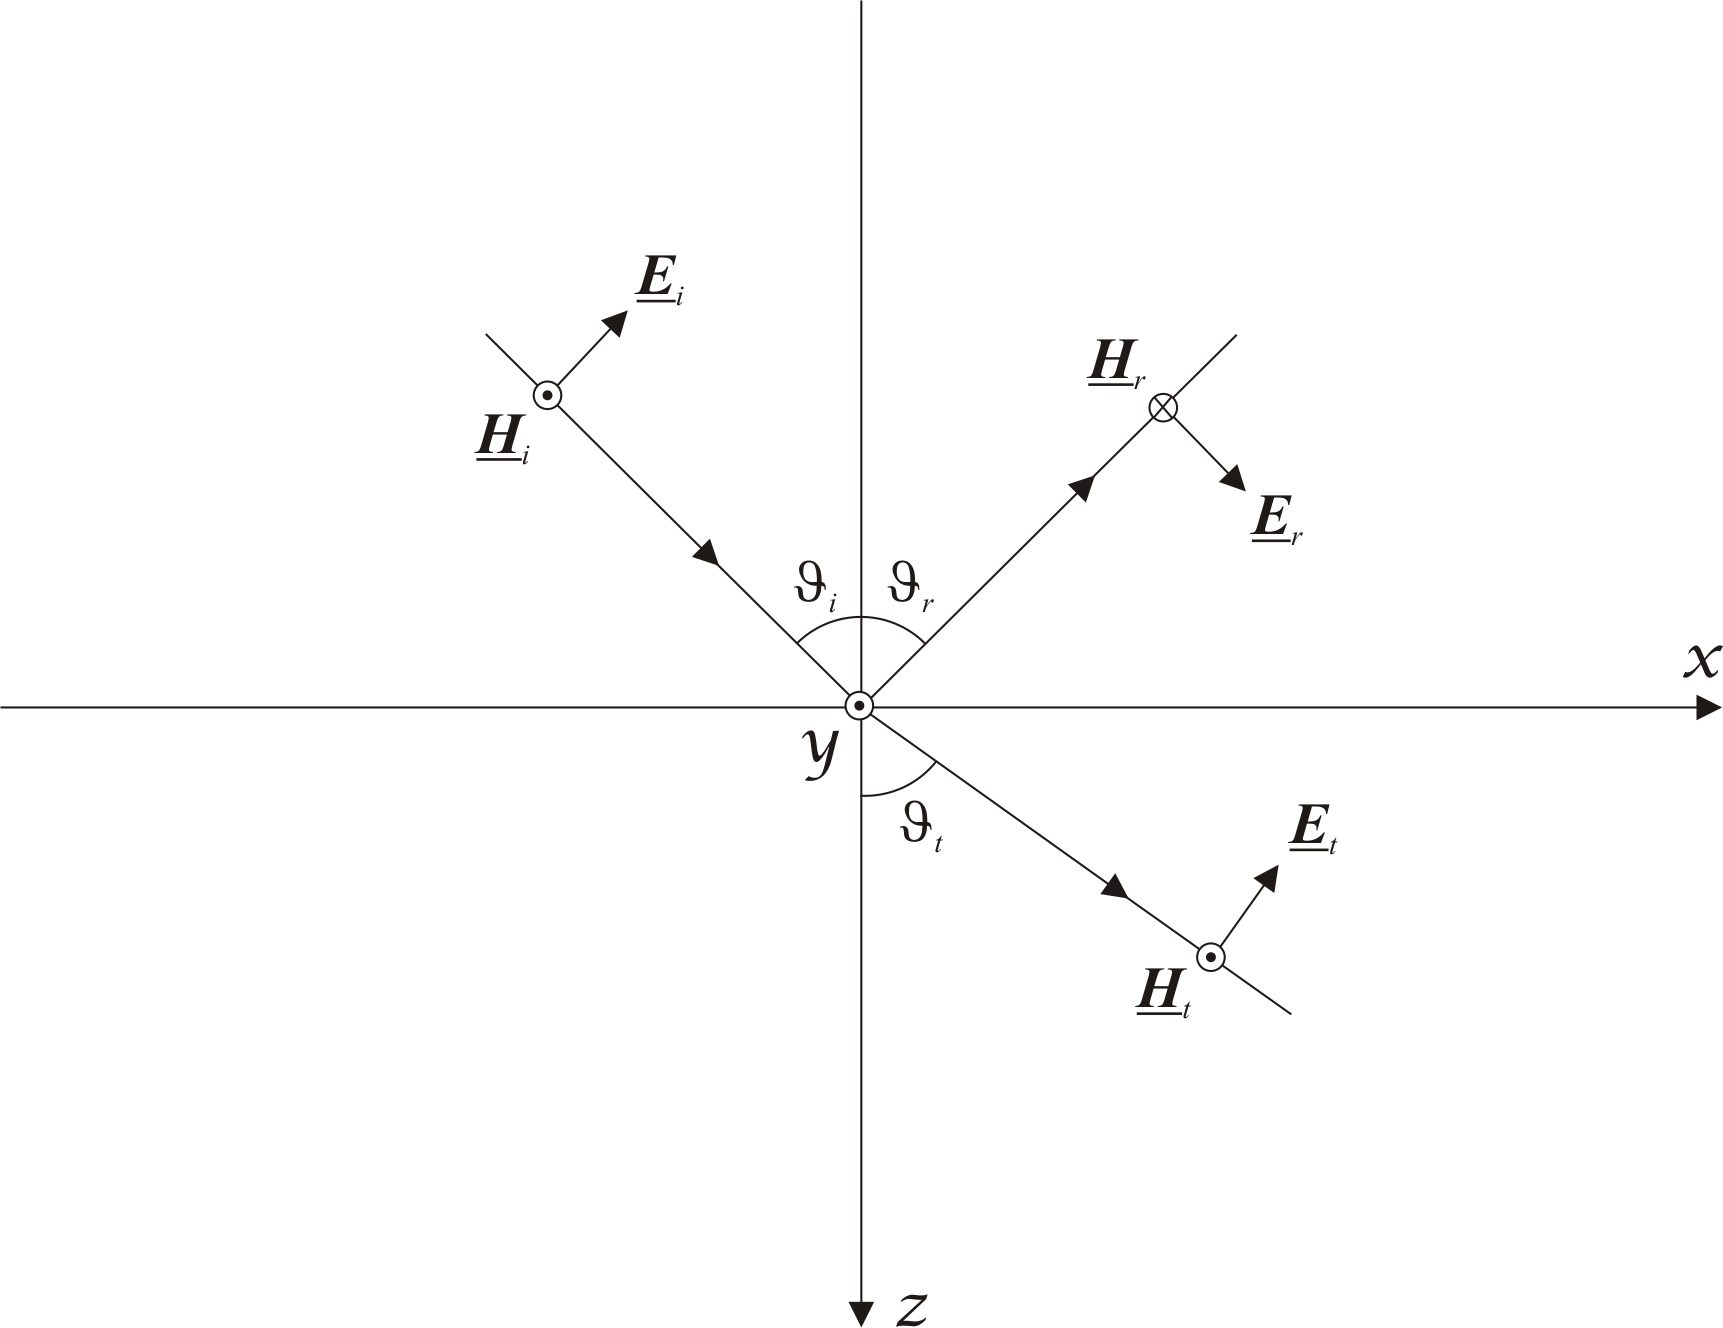
\includegraphics[width=11cm]{evlny_rovnobezna_polarizace.png}
	\caption{Rovnoběžná polarizace rovinné vlny. \cite{emp}}
	\label{obr:evlny_rovnobezna_polarizace}
\end{figure}
Odvození vztahů pro činitele odrazu a prostupu se nachází v~\cite[str. 95]{emp}. Pro výsledné vztahy platí v~tomto případě $\faz R_{\parallel} + 1 = \faz T_{\parallel}\frac{\cos\vartheta_{t}}{\cos\vartheta_{i}}$
\begin{equation}
	\faz R_{\parallel} = \frac{\faz E_{r0}}{\faz E_{i0}} = \frac{\faz Z_{2}\cos\vartheta_{t}-\faz Z_{1}\cos\vartheta_{i}}{\faz Z_{2}\cos\vartheta_{t}+\faz Z_{1}\cos\vartheta_{i}} = \frac{\faz Z_{2}\sqrt{1-(\faz k_{1}/\faz k_{2})^{2}\sin^{2}\vartheta_{i}}-\faz Z_{1}\cos\vartheta_{i}}{\faz Z_{2}\sqrt{1-(\faz k_{1}/\faz k_{2})^{2}\sin^{2}\vartheta_{i}}+\faz Z_{1}\cos\vartheta_{i}},
	\label{rce:evlny_cin_odrazu_rovnobezna}
\end{equation}
\begin{equation}
	\faz T_{\parallel} = \frac{\faz E_{t0}}{\faz E_{i0}} = \frac{2\faz Z_{2}\cos\vartheta_{i}}{\faz Z_{2}\cos\vartheta_{t}+\faz Z_{1}\cos\vartheta_{i}} = \frac{2\faz Z_{2}\cos\vartheta_{i}}{\faz Z_{2}\sqrt{1-(\faz k_{1}/\faz k_{2})^{2}\sin^{2}\vartheta_{i}}+\faz Z_{1}\cos\vartheta_{i}}.
	\label{rce:evlny_cin_prostupu_rovnobezna}
\end{equation}
Vztahy (\ref{rce:evlny_cin_odrazu_kolma}) až (\ref{rce:evlny_cin_prostupu_rovnobezna}) se také nazývají {\bf Fresnelovy rovnice}.

\subsection{Brewsterův polarizační úhel}
\subsubsection*{Situace u~kolmé polarizace dopadající vlny}
Úhel $\vartheta_{i}$ se označuje jako Brewsterův polarizační při splnění určitých podmínek. Pokud obecně polarizovaná elektromagnetická vlna dopadne na rozhraní pod tímto úhlem, tak odražená vlna bude mít pouze složku rovnoběžnou s~rovinou dopadu $xz$.

Odvození vychází ze vztahu pro $\faz R_{\perp}$ (\ref{rce:evlny_cin_odrazu_kolma}). Pokud bude platit $\faz Z_{2}\cos\vartheta_{i} = \faz Z_{1}\cos\vartheta_{t}$, tak činitel odrazu $\faz R_{\perp}$ vyjde nulový. To mimo jiné znamená, že se kolmo polarizovaná vlna neodráží a úplně celá prostupuje do druhého prostředí. Pomocí zákona lomu (\ref{rce:evlny_zakon_lomu}) a~vztahu $\cos\vartheta_{t} = \sqrt{1-\sin^{2}\vartheta_{t}}$ dostaneme
\begin{equation}
	\faz Z_{2}\cos\vartheta_{i} = \faz Z_{1}\sqrt{1-\bigg(\frac{\faz k_{1}}{\faz k_{2}}\bigg)^{2}\sin^{2}\vartheta_{i}}.
	\label{rce:evlny_brewster_kolma_odvozeni}
\end{equation}
Tento vztah (\ref{rce:evlny_brewster_kolma_odvozeni}) má řešení pro prostředí, kde platí $\mu_{1} \ne \mu_{2}$ a zároveň $\varepsilon_{1} = \varepsilon_{2}$. Výsledný výraz pro {\bf Brewsterův polarizační úhel} platí tedy pro tuto závislost materiálových konstant
\begin{equation}
	\sin\vartheta_{i\ BR} = \frac{1}{\sqrt{1+\frac{\mu_{1}}{\mu_{2}}}}.
	\label{rce:evlny_brewster_kolma}
\end{equation}

\subsubsection*{Rovnoběžná polarizace dopadající vlny}
Analogickým postupem jako v~předchozím případě vycházíme ze vztahu (\ref{rce:evlny_cin_odrazu_rovnobezna}) pro $\faz R_{\parallel}$. Zde se pro $\faz Z_{2}\cos\vartheta_{t} = \faz Z_{1}\cos\vartheta_{i}$ neodráží rovnoběžně polarizovaná vlna. Vztah Brewsterova polarizačního úhlu platí pro dielektrika ($\varepsilon_{1} \ne \varepsilon_{2}$), kde se po dopadu obecně polarizované vlny odráží složka polarizovaná kolmo na rovinu dopadu $xz$
\begin{equation}
	\sin\vartheta_{i\ BR} = \frac{1}{\sqrt{1+\frac{\varepsilon_{1}}{\varepsilon_{2}}}}.
	\label{rce:evlny_brewster_kolma}
\end{equation}
\newpage

\section{Vrstvené prostředí}
Při šíření elektromagentických vln v~reálných prostředích běžně dochází k~jevům na rozhraních. Ty jsou uvedeny v~podkapitole \ref{sec:evlny_rozhrani_dvou_prostredi}. V~praxi ale také může dojít k~přechodu vlny přes několik rozhraní za sebou, ať už se jedná o~požadovanou nebo nechtěnou funkci. Typicky se to týká šíření přes několik vrstev materiálu s~odlišnými parametry.

V~modelovém případě na obrázku \ref{obr:evlny_vrstvene_rada} se kolmo dopadající rovinná vlna $\vecfaz E_{i}$ částečně odráží a část proniká do prostředí popsaného vlnovou impedancí $\faz Z_{2}$. Zde může dále docházet k~mnohočetným odrazům. Prostupující vlna $\vecfaz E_{t}$ se nejprve odrazí od následujícího rozhraní $r_{23}$ jako $\vecfaz E_{tr}$. Poté může dojít na rozhraní $r_{12}$  k~průniku ($\vecfaz E_{trt}$) a dalšímu odrazu ($\vecfaz E_{trr}$) již původně odražené vlny. Tento proces se může opakovat dokud vlna v~daném prostředí nezanikne. Výsledná intenzita $\vecfaz E$ je pak dána součtem jednotlivých vln, které se vlivem odrazů a prostupů odráží. Vyjádření odražené vlny v~místě popsaném parametry s~indexem 1
\begin{equation}
	\vecfaz E_{1}^{-} = \vecfaz E_{r} + \vecfaz E_{trt} + \vecfaz E_{trrrt} + \cdots.
	\label{rce:evlny_vrstvene_rada1}
\end{equation}
Analogicky pro postupnou vlnu prostřední oblasti platí
\begin{equation}
	\vecfaz E_{2}^{+} = \vecfaz E_{t} + \vecfaz E_{trr} + \vecfaz E_{trrrr} + \cdots.
	\label{rce:evlny_vrstvene_rada2}
\end{equation}
\begin{figure}[!h]
	\centering
	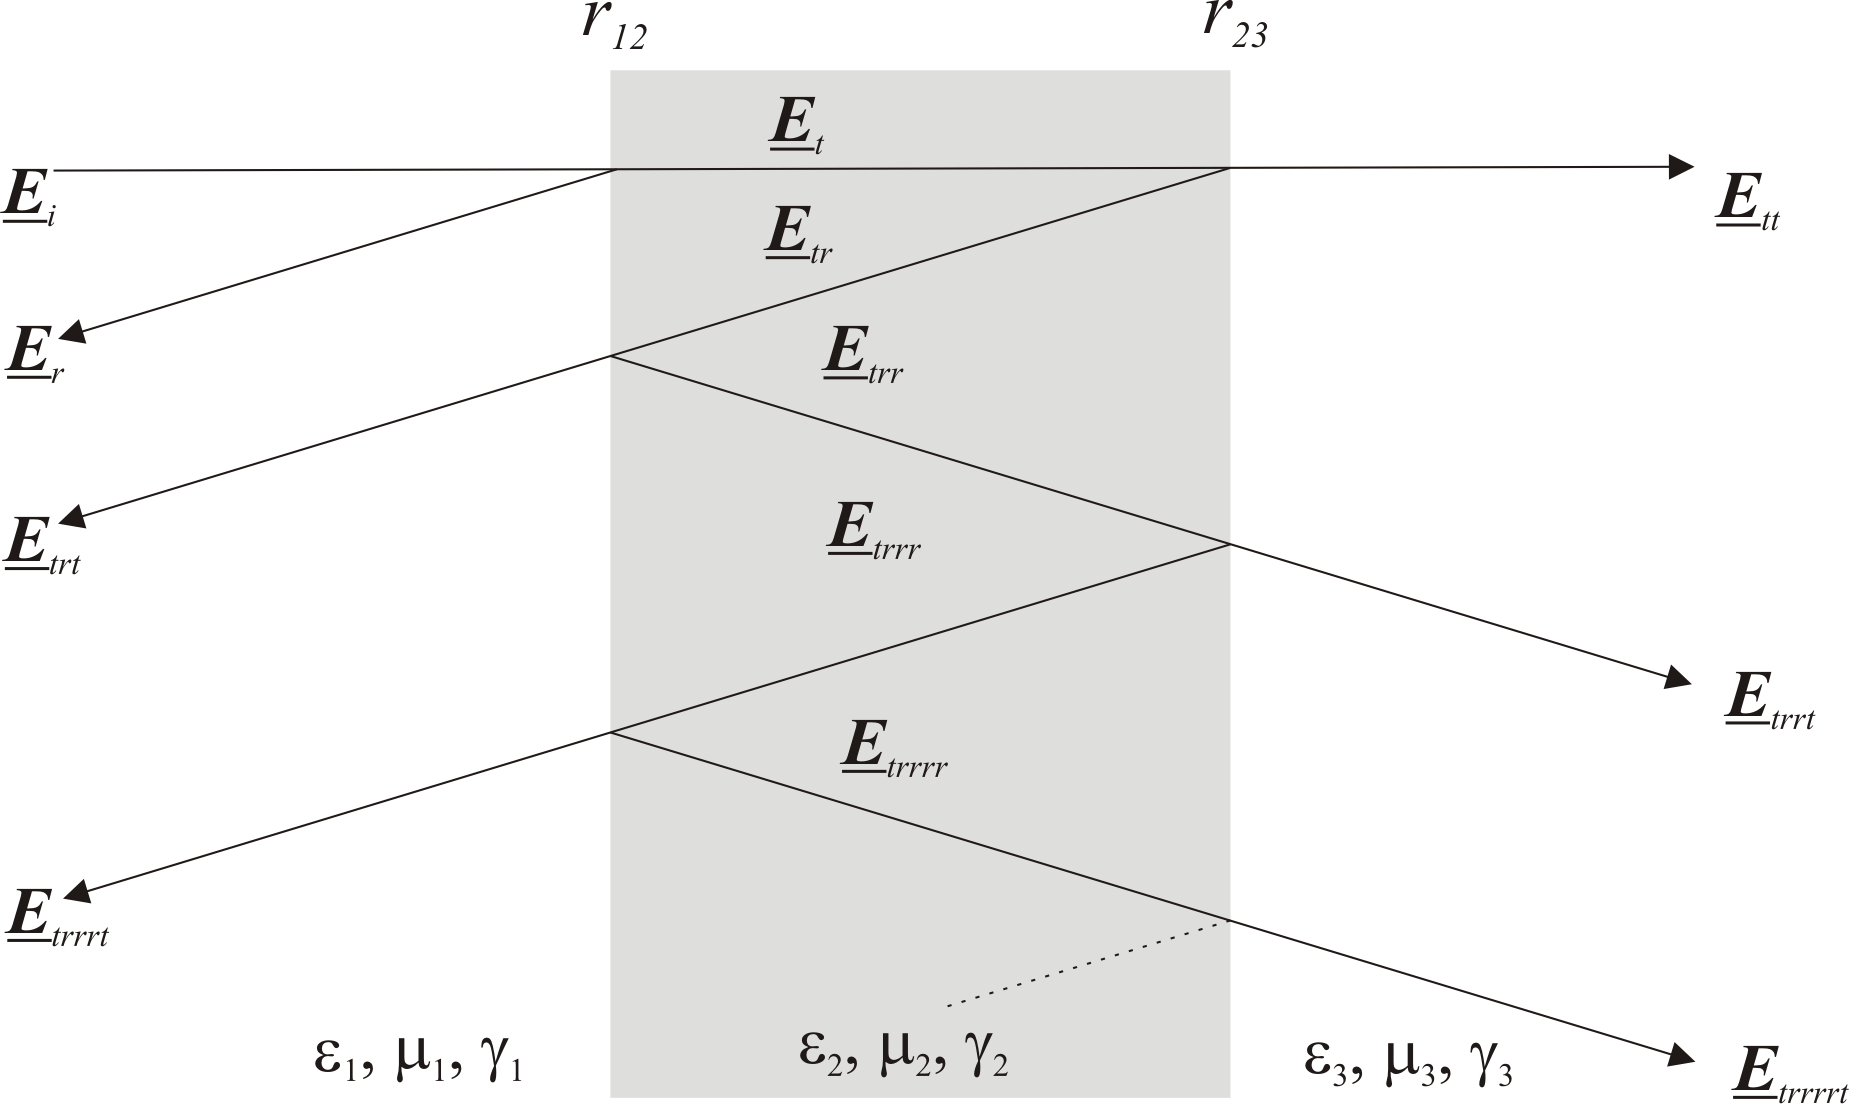
\includegraphics[width=12cm]{evlny_vrstvene_rada.png}
	\caption{Šíření elektromagnetických vln ve vrstveném prostředí. \cite{emp}}
	\label{obr:evlny_vrstvene_rada}
\end{figure}

\subsection{Metody řešení vln ve vrstveném prostředí}
Řešení chování elektromagnetické vlny vychází z~vyčíslení řad (\ref{rce:evlny_vrstvene_rada1}), (\ref{rce:evlny_vrstvene_rada2}), případně dalších. To je samo o~sobě ve většině případech velmi komplikované. Jednotlivé členy je pak potřeba sečíst s~ohledem na amplitudu a fázi. Pro další řešení existuje několik metod.
\begin{enumerate}
\item Součet vln stejného směru a vyjádření jedinou vlnou.
\item Maticová metoda.
\item Princip založený na transformaci vlnových impedancí.
\end{enumerate}

\subsubsection*{1. Součet vln stejného směru}
Postup této metody je blíže vysvětlen na příkladu v~\cite[str. 103 - 104]{emp}. V~každém prostředí, ve kterém se liší vlnová impedance $\faz Z$, se vyčíslí veškeré šířící se vlny. Například pro prostředí 1 na obrázku \ref{obr:evlny_vrstvene_rada} lze vyjádřit postupnou vlnu jako $\vecfaz E_{i}$ a odražená pak odpovídá výrazu (\ref{rce:evlny_vrstvene_rada1}). V~posledním prostředí uvažujeme pouze prostupující vlnu. Vyjádří se intenzita jak elektrického, tak i magnetického pole. Výsledné vlny se následně přizpůsobí podmínkám na rozhraní. Dostaneme soustavu, která bude mít počet rovnic závislý na počtu různých prostředí, přes které se elektromagnetická vlna šíří.

\begin{table}[!h]
\catcode`\-=12 
\begin{center}
  	\caption{Závislost počtu rovnic v~soustavě na vrstvách rozhraní.}
  	\label{tab:evlny_vrstvene_prostredi}
\begin{tabular}{|l|l|l|l|}
	\hline
	index & prostředí & počet rovnic & neznámých \\
	\hline
	0 & 2 & 2 & 3 \\
	1 & 3 & 4 & 5 \\
	2 & 4 & 6 & 7 \\
	\vdots & \vdots & \vdots & \vdots \\
	n & n+2 & 2n+2 & 2n+3 \\
	\hline
\end{tabular}
\end{center}
\end{table}

Pro tři prostředí (dle obrázku \ref{obr:evlny_vrstvene_rada}) dostaneme soustavu čtyř rovnic o~pěti neznámých. Aby ji bylo možné vyřešit, je potřeba znát alespoň jednu z~postupných nebo odražených vln. Ve většině případech je známá dopadající vlna $\vecfaz E_{i}$. 

\subsubsection*{2. Maticová metoda}
Je zřejmé, že první uvedená metoda bude s~nárůstem počtu vrstev čím dál více složitější. Postup další varianty řešení je opět rozebrán v~\cite[str. 105]{emp}. Tato metoda, jak už název napovídá, využívá matic. Pokud dopadají na rozhraní vlny z~obou stran podle obrázku \ref{obr:evlny_maticova_metoda1} je možné odvodit následující maticový tvar
\begin{equation}
\left[ \begin{array}{c}
\faz E_{1}^{+} \\
\faz E_{1}^{-} \\
\end{array} \right]
= 
\frac{1}{\faz T_ {12}}
\left[ \begin{array}{cc}
1 & \faz R_{12} \\
\faz R_{12} & 1 \\
\end{array} \right]
\cdot
\left[ \begin{array}{c}
\faz E_{2}^{+} \\
\faz E_{2}^{-} \\
\end{array} \right],
\label{rce:evlny_maticova_rozhrani}
\end{equation}
kde $\faz R_{12}$ představuje činitel odrazu a $\faz T_ {12}$ činitel prostupu při průchodu elektromagnetické vlny z~prostředí 1 do 2. 
\begin{figure}[!h]
	\centering
	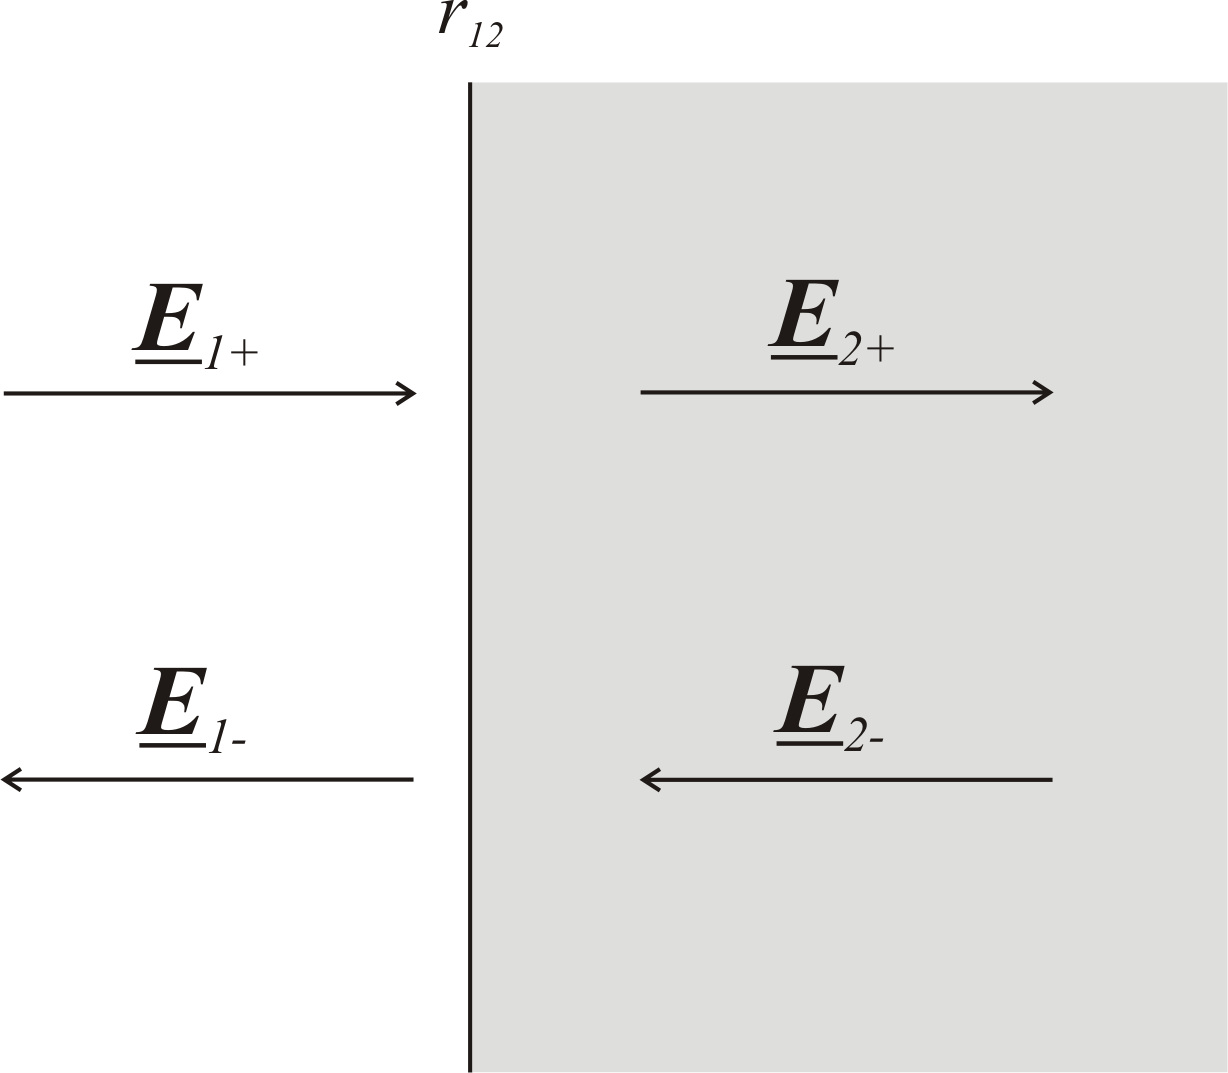
\includegraphics[width=5.5cm]{evlny_maticova_metoda1.png}
	\caption{Vlny dopadající na rozhraní z~obou stran. \cite{emp}}
	\label{obr:evlny_maticova_metoda1}
\end{figure}

Pokud bude vlna procházet vrstvou o~tloušťce $d$, ve které je popsána konstantou šíření $\faz k$, je opět možné podle situace na obrázku \ref{obr:evlny_maticova_metoda2} získat maticový zápis
\begin{equation}
\left[ \begin{array}{c}
\faz E_{2}^{+} \\
\faz E_{1}^{-} \\
\end{array} \right]
=
\left[ \begin{array}{cc}
\me^{\mj\faz k~d} & 0 \\
0 & \me^{-\mj\faz k~d} \\
\end{array} \right]
\cdot
\left[ \begin{array}{c}
\faz E_{3}^{+} \\
0 \\
\end{array} \right].
\label{rce:evlny_maticova_pruchod}
\end{equation}
\begin{figure}[!h]
	\centering
	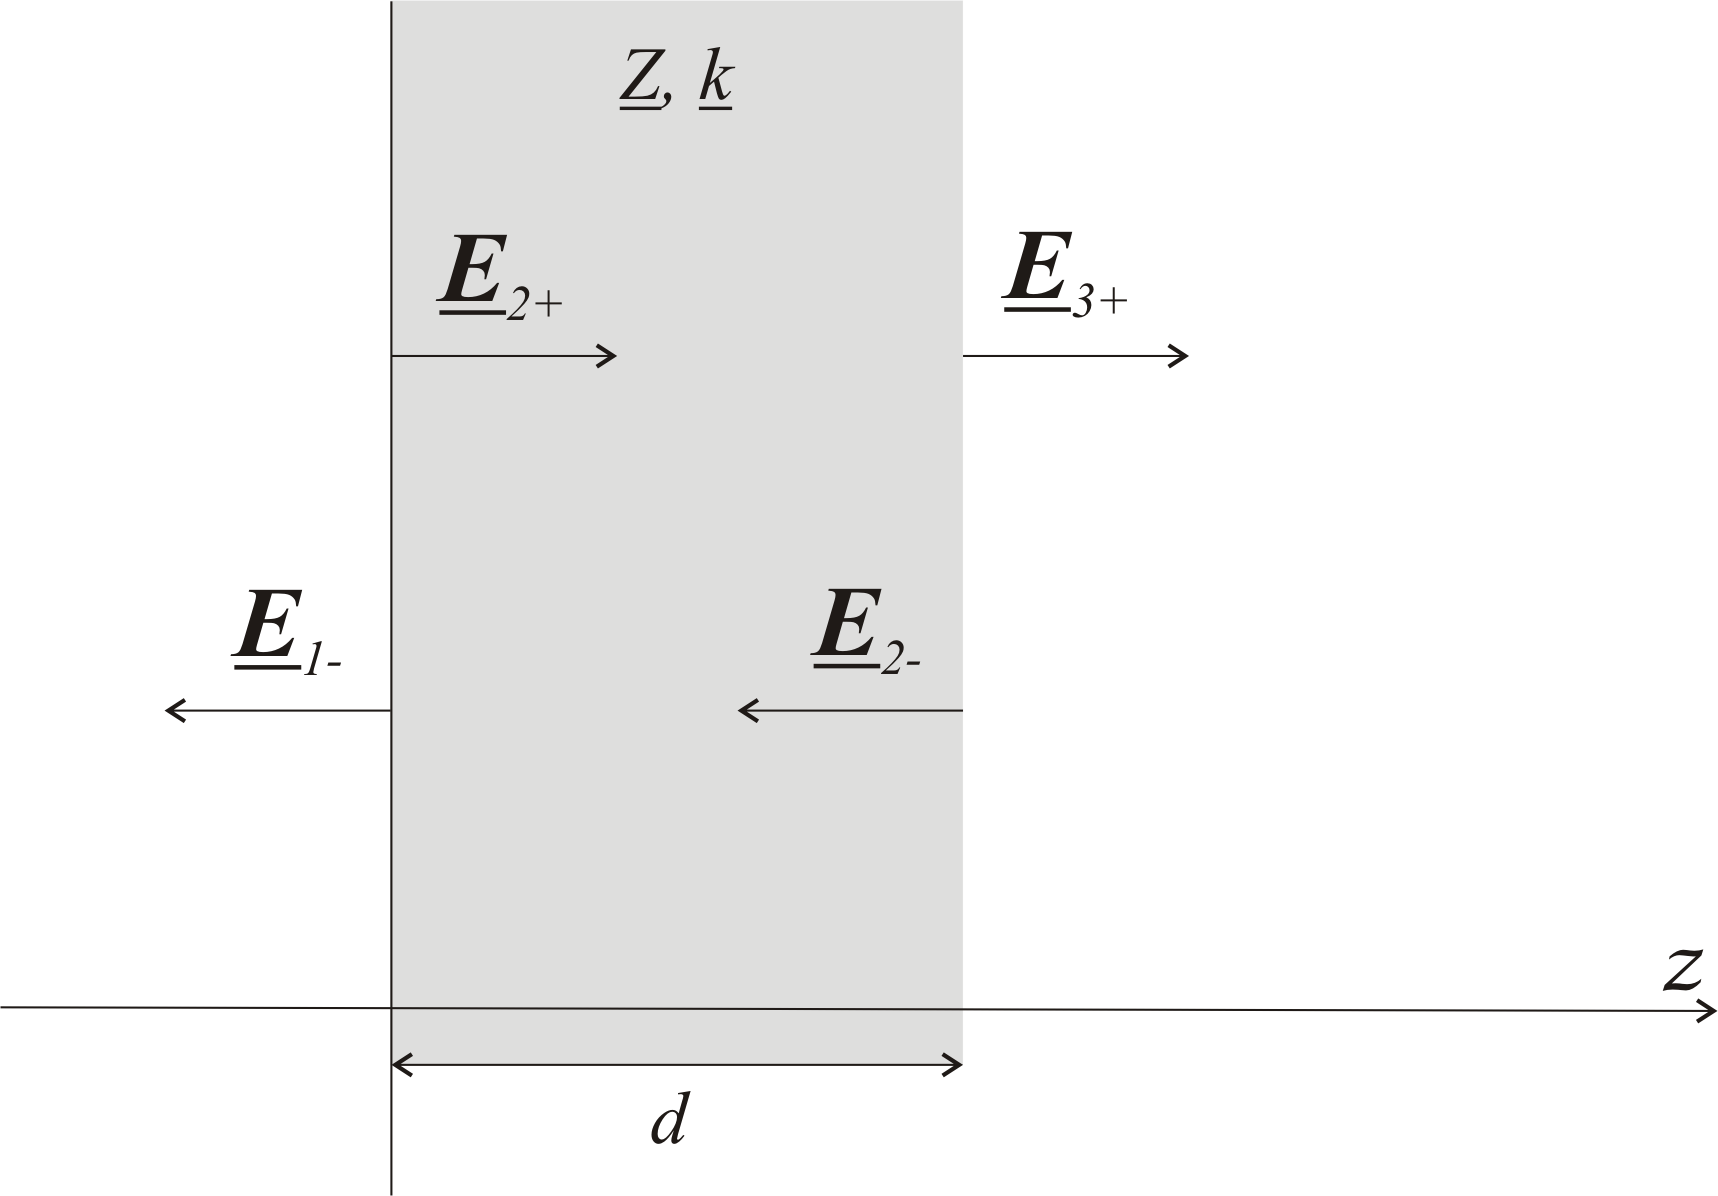
\includegraphics[width=8cm]{evlny_maticova_metoda2.png}
	\caption{Vlna procházející prostředím o~tloušťce $d$. \cite{emp}}
	\label{obr:evlny_maticova_metoda2}
\end{figure}

V~případě složité kombinace několika vrstev prostředí se využívá odvozených vztahů (\ref{rce:evlny_maticova_rozhrani}) a (\ref{rce:evlny_maticova_pruchod}) tak, že se postupně za sebou násobí takové matice, podle toho na jaké rozhraní elektromagnetická vlna dopadá a jakým prostředím prochází. Příklad šíření je uveden na obrázku \ref{obr:evlny_maticova_metoda3}. Vlna, šířící se z~prostředí 1 do prostředí 4, projde přes dvě oblasti o~tloušťce $d_{1}$, $d_{2}$ a tři rozhraní $r_{12}$, $r_{23}$ a $r_{34}$. Pro výslednou sestavu matic platí 
\begin{displaymath}
\left[ \begin{array}{c}
\faz E_{1}^{+} \\
\faz E_{1}^{-} \\
\end{array} \right]
=
\frac{1}{\faz T_ {12}}
\left[ \begin{array}{cc}
1 & \faz R_{12} \\
\faz R_{12} & 1 \\
\end{array} \right]
\cdot
\left[ \begin{array}{cc}
\me^{\mj\faz k_{2} d_{1}} & 0 \\
0 & \me^{-\mj\faz k_{2} d_{1}} \\
\end{array} \right]
\cdot
\frac{1}{\faz T_ {23}}
\left[ \begin{array}{cc}
1 & \faz R_{23} \\
\faz R_{23} & 1 \\
\end{array} \right]
\cdot
\end{displaymath}

\begin{equation}
\cdot
\left[ \begin{array}{cc}
\me^{\mj\faz k_{3} d_{2}} & 0 \\
0 & \me^{-\mj\faz k_{3} d_{2}} \\
\end{array} \right]
\cdot
\frac{1}{\faz T_ {34}}
\left[ \begin{array}{cc}
1 & \faz R_{34} \\
\faz R_{34} & 1 \\
\end{array} \right]
\cdot
\left[ \begin{array}{c}
\faz E_{4}^{+} \\
0 \\
\end{array} \right].
\end{equation} 
\begin{figure}[!h]
	\centering
	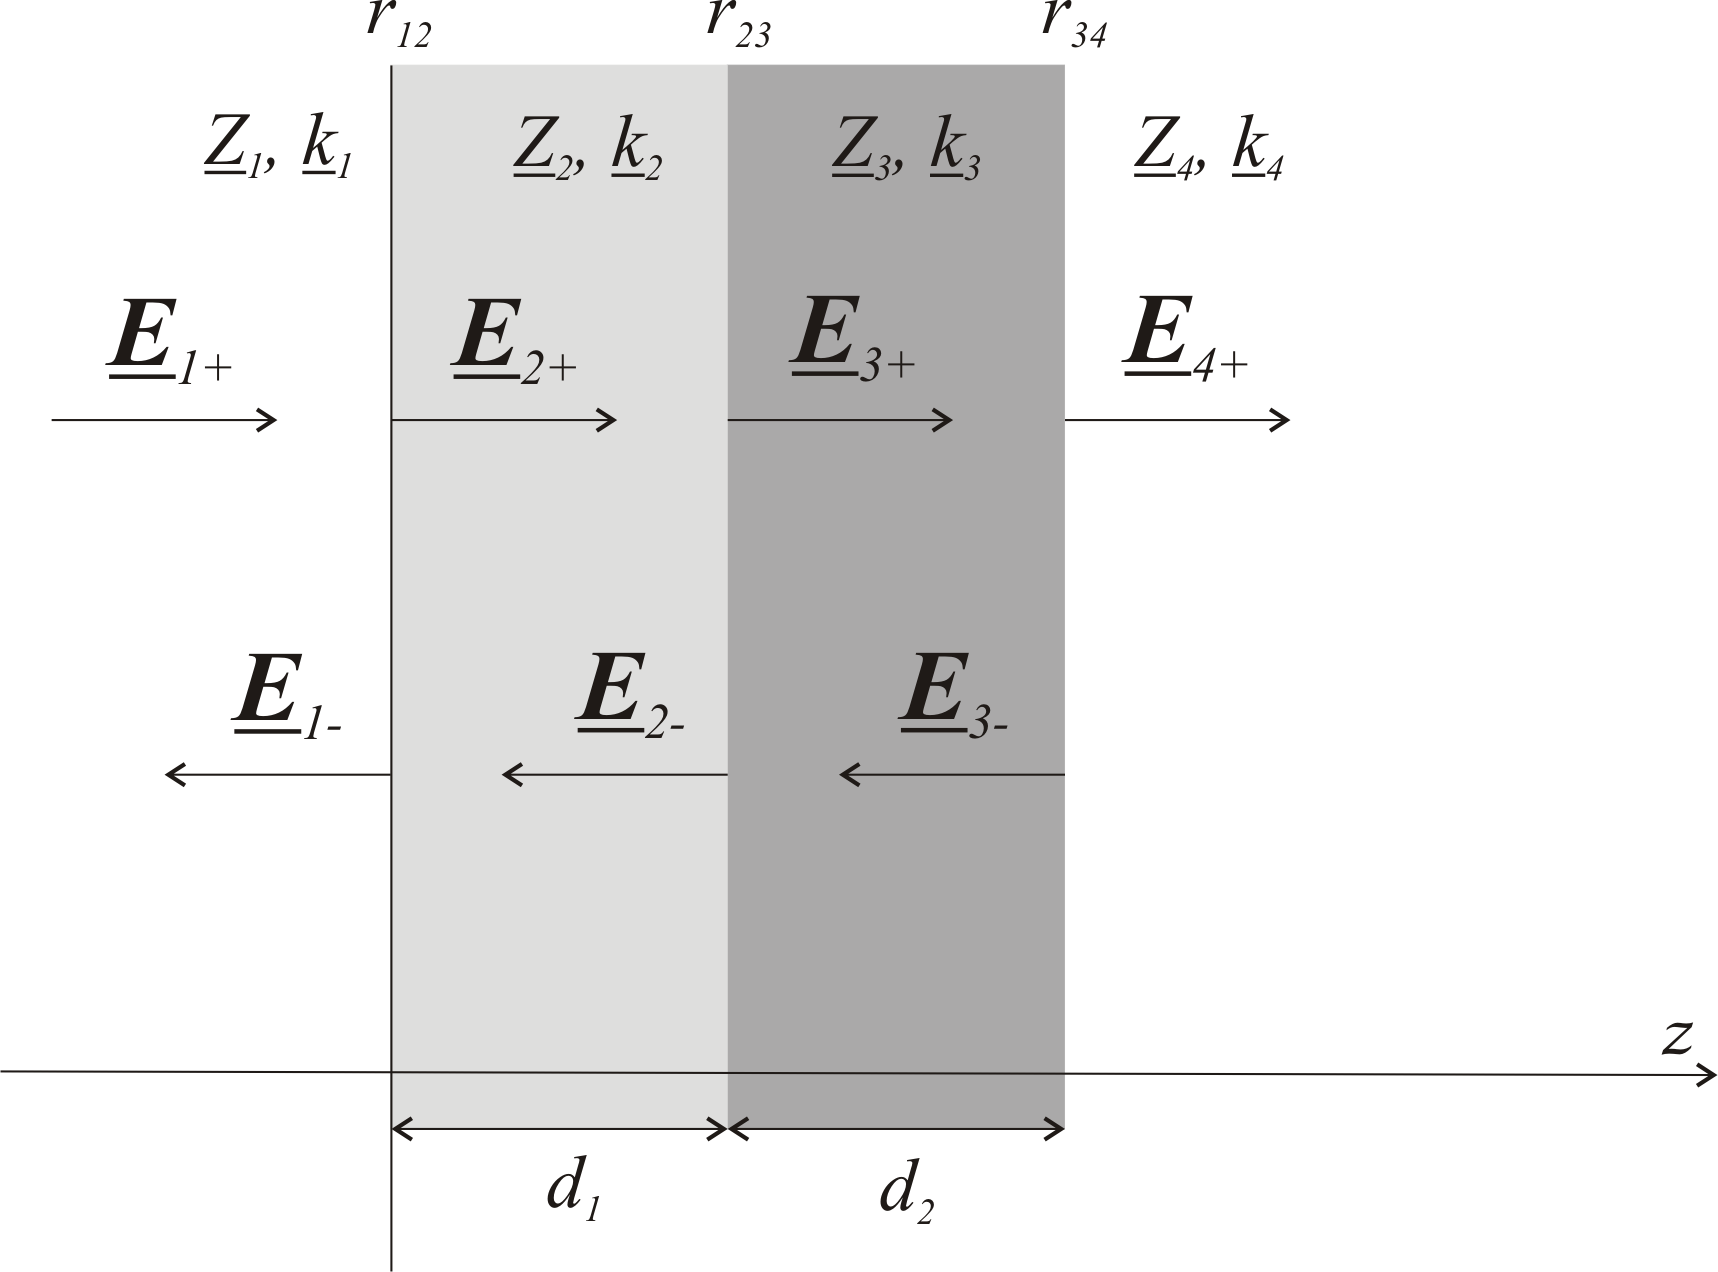
\includegraphics[width=8cm]{evlny_maticova_metoda3.png}
	\caption{Příklad vlny procházející přes dvě oblasti $d_{1}$ a $d_{2}$.}
	\label{obr:evlny_maticova_metoda3}
\end{figure}

\subsubsection*{3. Transformace vlnových impedancí}
Další možnost pro řešení vícevrstvých rozhraní vychází z~postupů, které se používají v~teorii vedení. Principem této metody je v~každém kroku výpočtu transformovat vlnovou impedanci posledního prostředí do místa rozhraní s~předcházející vrstvou. 
Odvození používaných vzorců se nachází v~\cite[str. 106]{emp}.
Pro situaci na obrázku \ref{obr:evlny_maticova_metoda3} bude prvním krokem transformace impedance $\faz Z_{3}$ a $\faz Z_{4}$ na rozhraní $r_{23}$ podle vztahu
\begin{equation}
	\faz Z_{c3}(r_{23}) = \faz Z_{3}\frac{\faz Z_{4}\cos(\faz k_{3}d_{2})+\mj\faz Z_{3}\sin(\faz k_{3}d_{2})}{\faz Z_{3}\cos(\faz k_{3}d_{2})+\mj\faz Z_{4}\sin(\faz k_{3}d_{2})}\unit{[\Omega]}.
	\label{rce:elvny_vrstvene_transformace1}
\end{equation}
V~dalším kroku se analogickým způsobem vypočtená impedance z~výrazu (\ref{rce:elvny_vrstvene_transformace1}) přepočte na rozhraní $r_{12}$
\begin{equation}
	\faz Z_{c2}(r_{12}) = \faz Z_{2}\frac{\faz Z_{c3}(r_{23})\cos(\faz k_{2}d_{1})+\mj\faz Z_{2}\sin(\faz k_{2}d_{1})}{\faz Z_{2}\cos(\faz k_{2}d_{1})+\mj\faz Z_{c3}(r_{23})\sin(\faz k_{2}d_{1})}\unit{[\Omega]}.
	\label{rce:elvny_vrstvene_transformace2}
\end{equation}
Nakonec je možné definovat činitele prostupu (\ref{rce:evlny_cin_prostupu}) a odrazu (\ref{rce:evlny_cin_odrazu}) na rozhraní $r_{12}$
\begin{equation}
	\faz R = \frac{\faz Z_{c2}(r_{12}) - \faz Z_{1}}{\faz Z_{1} + \faz Z_{c2}(r_{12})}
	\label{rce:elvny_vrstvene_transf_R},
\end{equation}
\begin{equation}
	\faz T = \frac{2\faz Z_{c2}(r_{12})}{\faz Z_{1} + \faz Z_{c2}(r_{12})}
	\label{rce:elvny_vrstvene_transf_T}.
\end{equation}
\newpage

\section{Vlnovody}
Během šíření vln ve volném prostředí od zdroje k~přijímací anténě dochází přirozeně k~rozptylu energie do prostoru. Anténou je tak zachycena pouze její část. To platí i pro směrové vysílací antény, pokud přenos probíhá na velké vzdálenosti. Pro zvýšení jeho efektivity je potřeba použít nějaké konstrukce, která umožňuje vedení energie.

To je možné zprostředkovat právě pomocí vlnovodů, jejichž nejběžnější provedení jsou na obrázku \ref{obr:evlny_vlnovody}. Vlnovody představují přípravek, ve kterém se elektromagnetická vlna šíří podélně ve směru osy $z$. V~příčném směru (tj. podle os $x$ a $y$) vzniká tzv. stojaté vlnění.
\begin{figure}[!h]
	\centering
	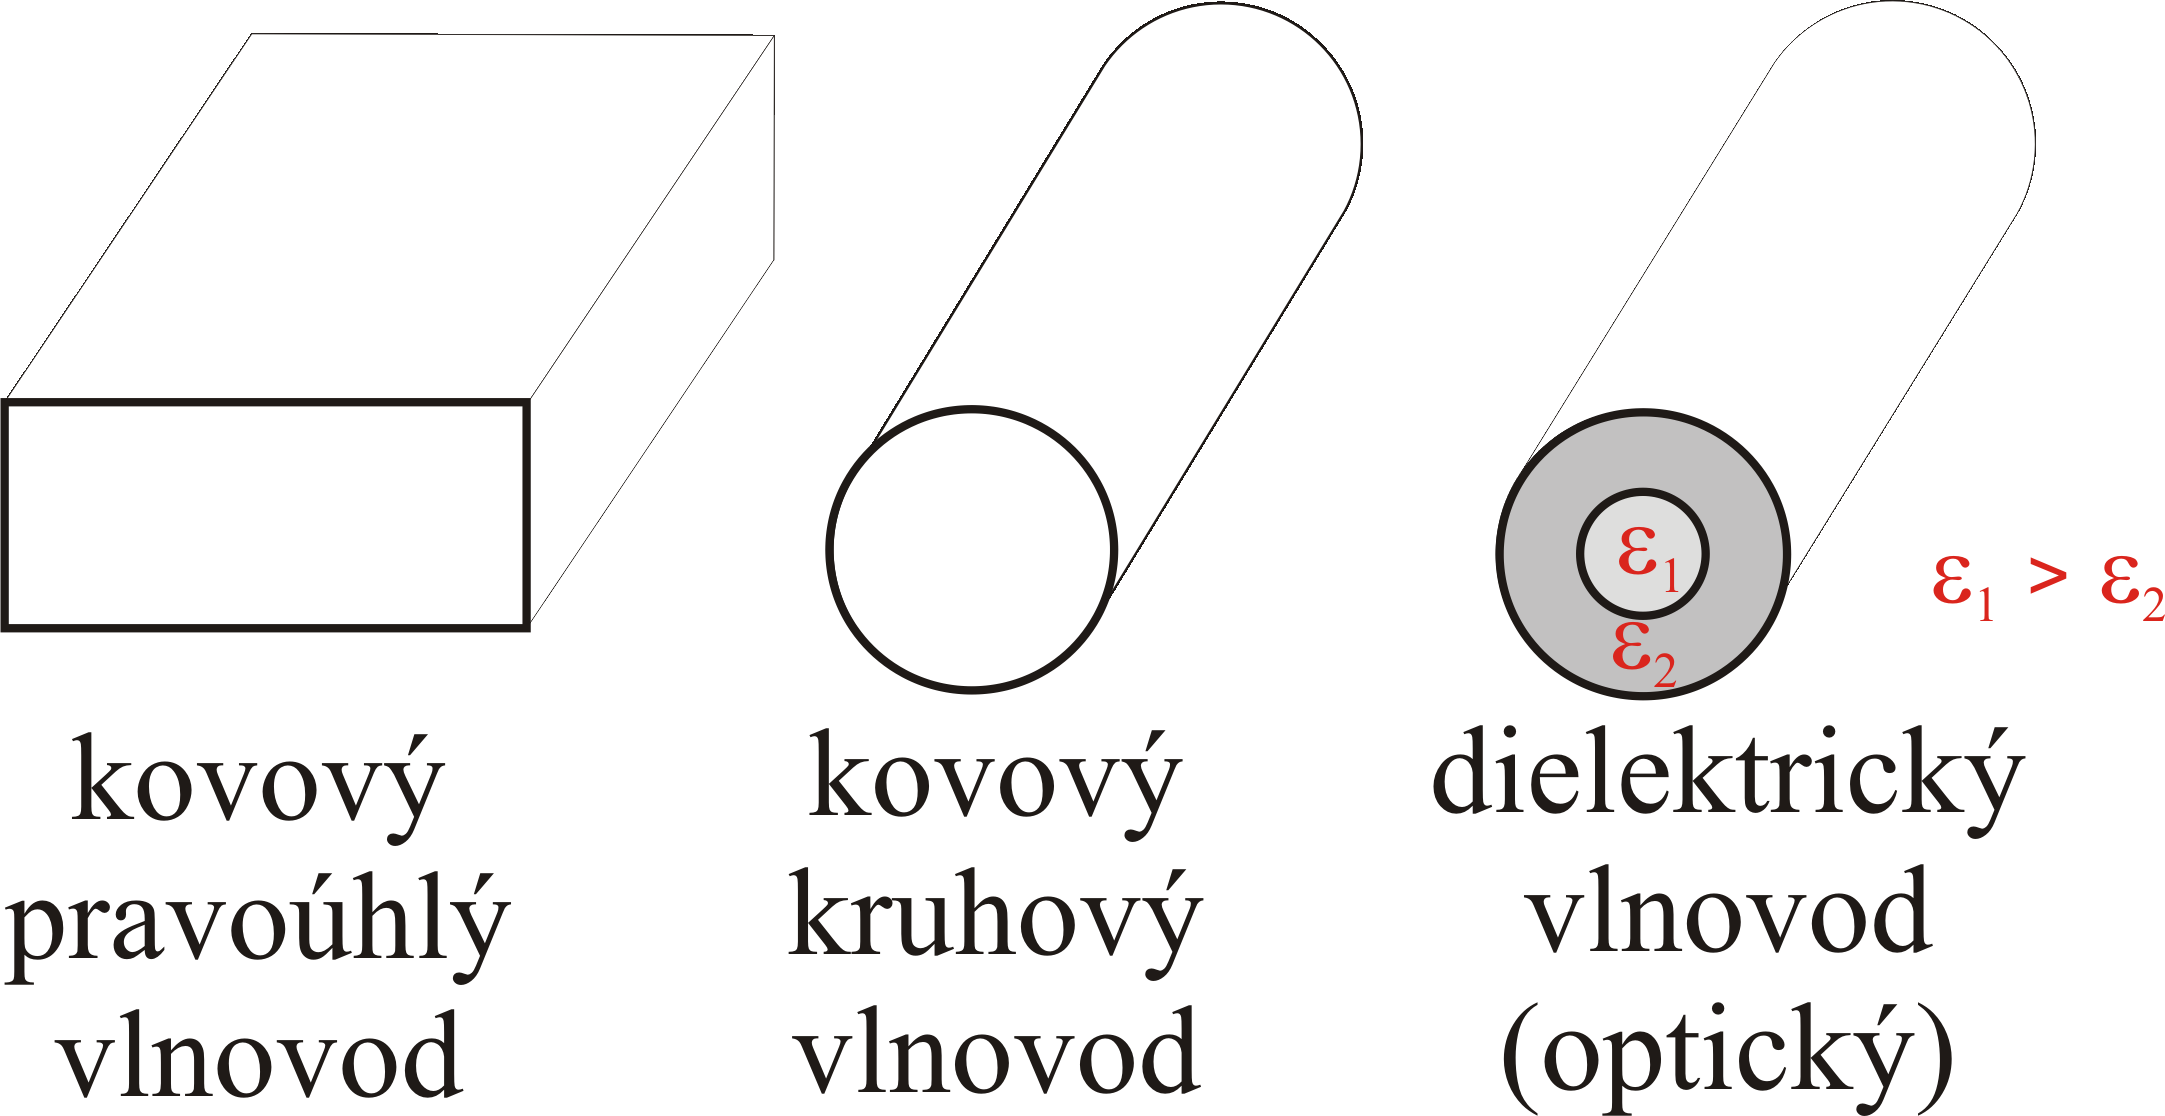
\includegraphics[width=6cm]{evlny_vlnovody.png}
	\caption{Nejběžnější konstrukce vlnovodů. \cite{emp}}
	\label{obr:evlny_vlnovody}
\end{figure}
Výhody vlnovodů jsou, kromě malých ztrát přenosu, v~nízké úrovni vyzařování do okolí  . Nevýhodou může být jejich cena a výroba pro velmi vysoké kmitočty. 

Další možnost pro přenos energie poskytují vedení, například dvouvodičnové, koaxiální nebo mikropáskové, které jsou popsané v~\cite{emp}.

\subsection{Klasifikace vln}
Vedené vlny lze rozlišit na několik druhů. Toto dělení se děje podle podélných složek pole, kterými jsou $\faz E_{z}$ a $\faz H_{z}$. V~případě vlnovodů se vnitřním prostorem šíří vlny typu TM a TE.

\subsubsection*{TEM vlny}
U~TEM, nebo-li transverzálně elektromagnetických vln jsou obě podélné složky pole nulové. Pro příčné složky, označené indexem $\perp$, platí dle \cite{emp} vztahy
\begin{displaymath}
	\nabla^{2}_{\perp} \vecfaz E_{\perp} = 0,\qquad\nabla^{2}_{\perp} \vecfaz H_{\perp} = 0.
\end{displaymath}
Charakterem odpovídají tyto rovnice elektrostatickému poli, proto i rozložení pole pro TEM vlny bude obdobné.

\subsubsection*{TM vlny}
Transverzálně magnetické nebo také elektrické vlny mají nulovou složku magnetického pole $\faz H_{z}$. Složka elektrického pole $\faz E_{z}$ je nenulová. Řešení pole vychází z~vlnové rovnice ve tvaru
\begin{displaymath}
	\nabla^{2} \faz E_{z} + \faz k^{2}\faz E_{z} = 0,
\end{displaymath}
kde $\faz k$ představuje konstatnu šíření ve volném prostoru. Ta se skládá z~podélné $\faz k_z$ a příčné $\faz k_p$ konstanty šíření. Mezi sebou jsou vázány vztahem $\faz k^{2} = \faz k_z^{2} + \faz k_p^{2}$. Pro impedanci vlnovodu $\faz Z_{V}$ platí pro TM vlny vztah
\begin{displaymath}
   \faz Z_{V}^{TM} = \frac{\faz k_z}{\omega\varepsilon}\unit{[\Omega]}.
\end{displaymath}

\subsubsection*{TE vlny}
TE označuje vlny transverzálně elektrické. To jsou takové, které mají $\faz E_{z} = 0$. Příslušná vlnová rovnice má tvar
\begin{displaymath}
	\nabla^{2} \faz H_{z} + \faz k^{2}\faz H_{z} = 0.
\end{displaymath}
Impedance vlnovodu pro TE vlny je
\begin{displaymath}
	\faz Z_{V}^{TE} = \frac{\omega\mu}{\faz k_z}\unit{[\Omega]}.
\end{displaymath} 
\subsubsection*{EH a HE vlny}
Tento typ vln se vyskytuje ve vlnovodech složených z~několika dielektrik. Mají obě podélné složky pole nenulové a někdy se také označují jako vlny hybridní. Podle poměru $\frac{\faz E_z}{\faz H_z}$ se rozlišuje označení EH nebo HE.

\subsection{Parametry vlnovodů obdélníkových průřezů}
Tento typ vlnovodu patří k~nejběžněji používaným. 
Pro příčnou konstantu $k_p$ platí 
\begin{displaymath}
	k_p = \sqrt{\bigg(\frac{m\pi}{a}\bigg)^{2} + \bigg(\frac{n\pi}{b}\bigg)^{2}},
\end{displaymath}
kde $m, n = 1, 2, 3,\cdots$. Hodnoty $a$ a $b$ představují geometrii vlnovodu.

\subsection*{Mezní (kritická) frekvence}
Aby mohla být elektromagnetická vlna vedena vlnovodem, je potřeba, aby její kmitočet byl vyšší než mezní, který je definován
\begin{equation}
f_{m} = \frac{c}{2\pi\sqrt{\varepsilon_{r}\mu_{r}}}\cdot k_p = \frac{c}{2\sqrt{\varepsilon_{r}\mu_{r}}}\cdot \sqrt{\bigg(\frac{m}{a}\bigg)^{2} + \bigg(\frac{n}{b}\bigg)^{2}}\unit{[Hz]}. 
	\label{rce:evlny_vlnovody_mezni_frekvence}
\end{equation}
Tato hodnota je stejná jak pro TM, tak i pro TE vlny.
\subsection*{Mezní (kritická) vlnová délka}
Pro vedení vlny musí být vlnová délka menší než mezní, pro kterou platí
\begin{equation}
\lambda_{m} = \frac{c}{f_{m}} = \frac{2\sqrt{\varepsilon_{r}\mu_{r}}}{\sqrt{\big(\frac{m}{a}\big)^{2} + \big(\frac{n}{b}\big)^{2}}}\unit{[m]}. 
	\label{rce:evlny_vlnovody_mezni_vlnova_delka}
\end{equation}
Vztah je opět stejný pro TM a TE vlny.
\subsection*{Impedance vlnovodu}
Velikost impedance vlnovodu závisí na typu šířících se vln. V~případě transverzálně magnetických platí
\begin{displaymath}
	\faz Z_{V}^{TM} = \frac{\faz k_z}{\omega\varepsilon} = \frac{\sqrt{k^{2} - \big(\frac{m}{a}\big)^{2} - \big(\frac{n}{b}\big)^{2}}}{\omega\varepsilon}\unit{[\Omega]}
\end{displaymath}
a pro TE vlny náleží vztah
\begin{displaymath}
	\faz Z_{V}^{TE} = \frac{\omega\mu}{\faz k_z} = \frac{\omega\mu}{\sqrt{k^{2} - \big(\frac{m}{a}\big)^{2} - \big(\frac{n}{b}\big)^{2}}}\unit{[\Omega]}.
\end{displaymath}

\section{Dutinové rezonátory}
V~elektrotechnice se běžně používají systémy, založené na principu rezonance. Pro nízké frekvence je lze zrealizovat pomocí vhodné kombinace indukčnosti L, kapacity C a odporu R. Ve vysokofrekvenční oblasti tento přístup není možný a funkci těchto systémů plní dutinové rezonátory. 

Významnou skupinu představují rezonátory vytvořené z~vlnovodů, kterým se uzavře vstupní a výstupní brána. Obecně se jedná o~objem dielektrika libovolného tvaru, který je uzavřen dobře vodivým pláštěm. V~praxi se však upřednostňují rezonátory jednoduchých geometrických forem, například pravoúhlé (obrázek \ref{obr:evlny_rezonator}), cylindrické nebo toroidiální. 
\begin{figure}[!h]
	\centering
	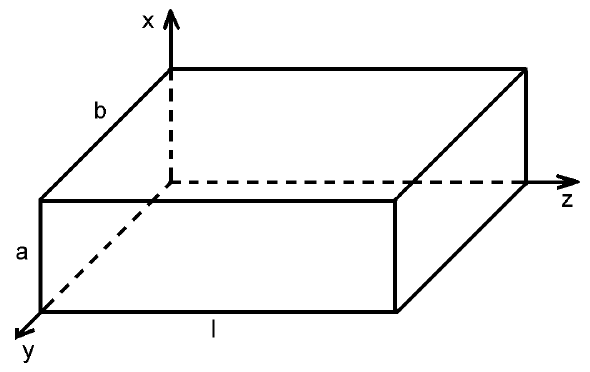
\includegraphics[width=5cm]{evlny_rezonator.png}
	\caption{Pravoúhlý dutinový rezonátor. \cite{tripak}}
	\label{obr:evlny_rezonator}
\end{figure}

Vzhledem ke skutečnosti, že rezonátory jsou uzavřený útvar, nedochází zde k~šíření vlny v~žádném směru. Mezi všemi stěnami se vyskytuje, podobně jako u~vlnovodů ve směru os $x$ a $y$, stojaté vlnění. U~rezonátorů tedy oproti vlnovodům existuje toto vlnění navíc i podél $z$-ové souřadnice. 

Analýzu jednotlivých typů rezonátorů je možné nalézt v~\cite{emp} nebo \cite{tripak}.

\subsection{Parametry rezonátorů}
Obdobně jako u~rezonančních systémů vytvořené z~R, L a C prvků, tak i u~dutinové rezonátory je možné charakterizovat několika parametry.
\subsection*{Rezonanční kmitočet}
\begin{displaymath}
	f_r = \frac{c}{2\sqrt{\varepsilon_r \mu_r}}\sqrt{\bigg(\frac{m}{a}\bigg)^{2} + \bigg(\frac{n}{b}\bigg)^{2} + \bigg(\frac{p}{d}\bigg)^{2}}\unit{[Hz]},
\end{displaymath}
kde $m, n, p = 1, 2, 3,\cdots$. Hodnoty $a$,$b$ a $d$ představují geometrii rezonátoru.
\subsection*{Kvalita (Jakost) rezonátoru}
Dalším důležitým parametrem rezonátoru se nazývá kvalita, případně jakost. Představuje míru ztrát energie za jednu periodu a je dána vztahem
\begin{displaymath}
	Q_0 = \omega_r \frac{W_{r}}{P},
\end{displaymath}
kde $\omega_r$ je úhlový rezonanční kmitočet, $W_r$ představuje nahromaděnou  energii a $P$ jsou výkonové ztráty v~rezonátoru.
\newpage

\chapter{Simulace} \label{kap:Simulace}
% !TeX root = Main.tex
Programový kód, kterým je realizována simulace šíření elektromagnetického pole, je proveden jako modul pro aplikaci Agros2D. Prostředí tohoto programu je patrné na obrázku \ref{obr:sim_agros2d}. Mezi základní prvky patří uprostřed umístěná pracovní plocha pro zadání geometrie řešeného problému a současně i prostor pro zobrazení výsledků. V~levé horní části se nachází informační okno o~daném řešeném problému včetně seznamu zadaných okrajových podmínek a materiálech. Pod tímto oknem je snadno dostupný postprocesor pro volbu zobrazení vyřešeného fyzikálního pole. Pravá oblast aplikace poskytuje možnost zobrazení hodnot konkrétních veličin v~požadovaném bodě.

\begin{figure}[!h]
	\centering
	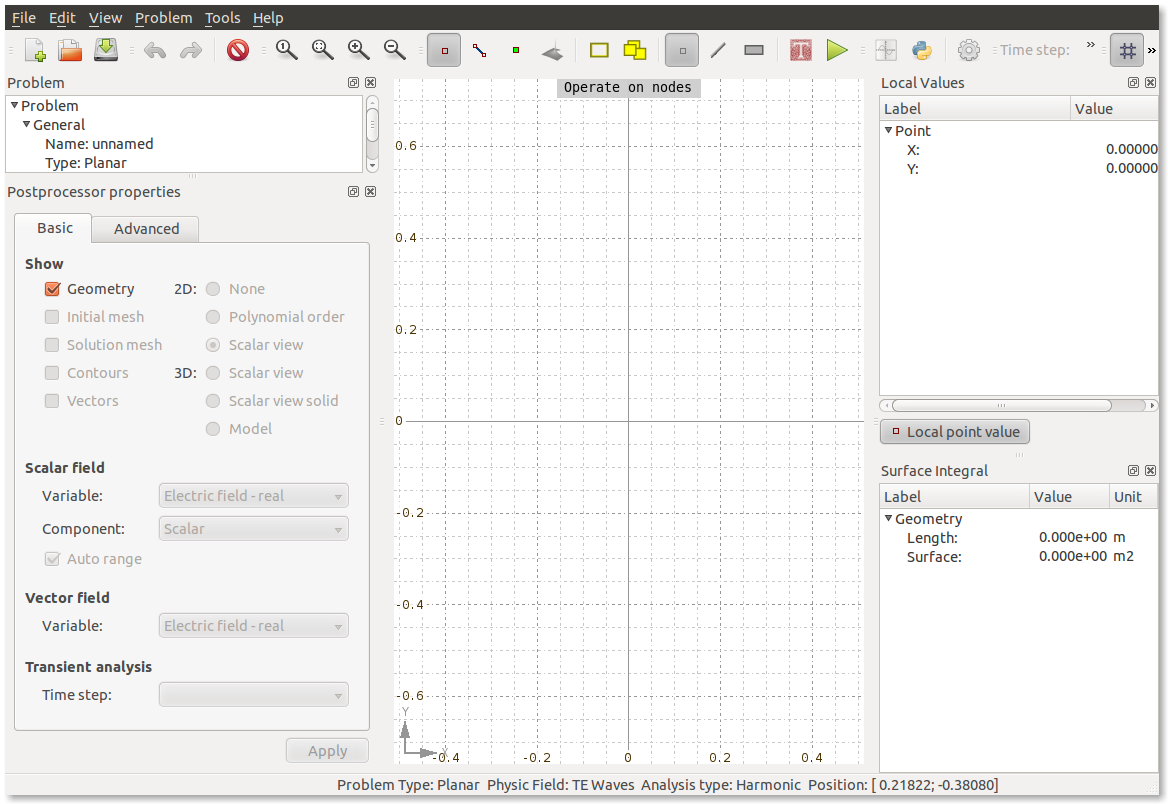
\includegraphics[width=14cm]{sim_agros2d.png}
	\caption{Základní pracovní rostředí programu Agros2D.}
	\label{obr:sim_agros2d}
\end{figure}

Samotný modul pro simulaci elektromagnetického pole tedy využívá z~programu Agros2D zmíněný preprocesor pro zadávání dat a postprocesor pro zobrazení výsledků ve 2D a 3D zobrazení. Vlastní numerické řešení zajišťuje knihovna Hermes2D a programový kód je obsažen v~ příslušném modulu. V~této kapitole jsou popsány výpočetní části, které se týkají především řešení vlnových rovnic, specifikace okrajových podmínek a zadávání materiálových konstant prostředí. 

\section{Metoda konečných prvků}
Základem samotné knihovny Hermes2D je numerické řešení pomocí tzv. metody konečných prvků neboli FEM (Finite Element Method). Historie spadá do první poloviny 20. století, kdy byly základy FEM popsány v~práci a Richarda Couranta (1943). Až v~roce 1953 byly rovnice popsány v~maticovém tvaru, což umožnilo řešení na počítačích a v~té době se FEM využívala v~leteckém průmyslu. K~jejímu šiřšímu využití v~dalších oborech však došlo až s~nástupem modernější výpočetní techniky v~průběhu 60. a 70. let. Například na problémy týkající se elektromagnetismu nebyla FEM použita dříve než v~roce 1968. V~současné době se však pomocí FEM výhodně řeší fyzikální problémy z~oborů statiky, dynamiky, akustiky, tepla, elektromagnetického pole, proudění, elektrostatiky a z~dalších vědeckých disciplín. 

Ačkoliv existují také jiné numerické metody řešení, například metoda konečných diferencí (FDM) nebo momentová metoda (MOM), které nejsou tak náročné na programovou implementaci, tak právě varianty metody FEM (v případě Hermes2D jde o $hp$-FEM) jsou nejvíce používané. Důvodem je jejich všestrannost a výkonnost. Dále také proto, že programy vyvinuté pro konkrétní problémy mohou být snadno použity k~řešení příkladů v~naprosto jiném oboru pomocí drobných nebo dokonce žádných změn.

\subsection{Kroky řešení pomocí FEM}
Analýza jakéhokoliv problému prostřednictvím metody konečných prvků zahrnuje v~podstatě čtyři kroky:
\begin{itemize}
\item {Diskretizace oblasti na konečný počet prvků.}
\item {Vyjádření rovnic pro konkrétní prvek.}
\item {Sestavení prvků v~řešené oblasti.}
\item {Řešení získaných rovnic.}
\end{itemize}
Vlatní princip řešení a odvození příslušných rovnic je možné nalézt v~\cite[kap. 6.2]{num}, kde je FEM pro jednoduchost reprezentována na Laplaceově rovnici $\nabla^{2}V = 0$ .

\subsection*{Diskretizace}
Prvním krokem pro numerické řešení rovnic je rozdělení nekonečného objemu řešené oblasti na konečný počet prvků, tak jak je to naznačeno na obrázku \ref{obr:sim_diskretizace}.
\begin{figure}[!h]
	\centering
	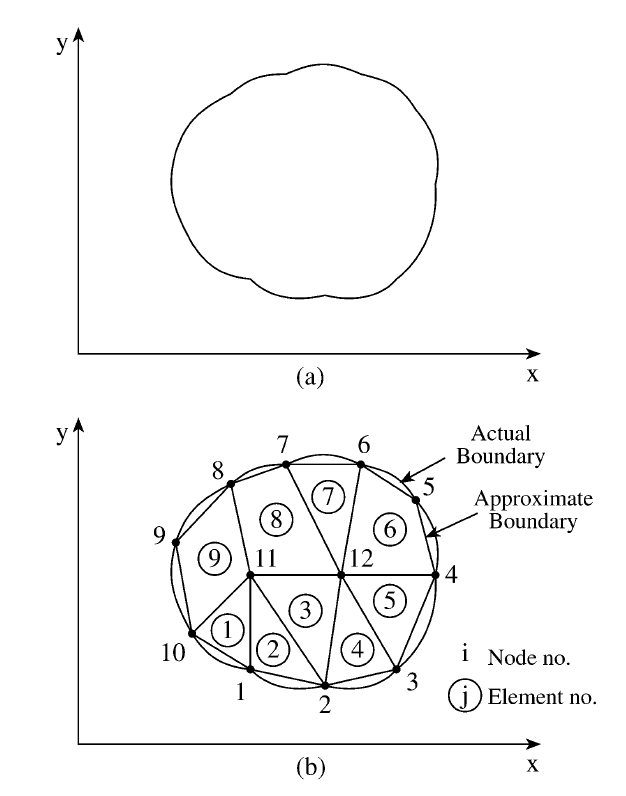
\includegraphics[width=13cm]{sim_diskretizace.png}
	\caption{Dělení řešené oblasti (a) na konečný počet diskretizačních prvků (b). \cite{num}}
	\label{obr:sim_diskretizace}
\end{figure}
Vlastní prvky, na které je oblast rozčleněna mohou mít libovolný tvar, ale typické tvary pro dvojdimenzionální problém jsou jsou naznačeny na obrázku \ref{obr:sim_prvky}.
\begin{figure}[!h]
	\centering
	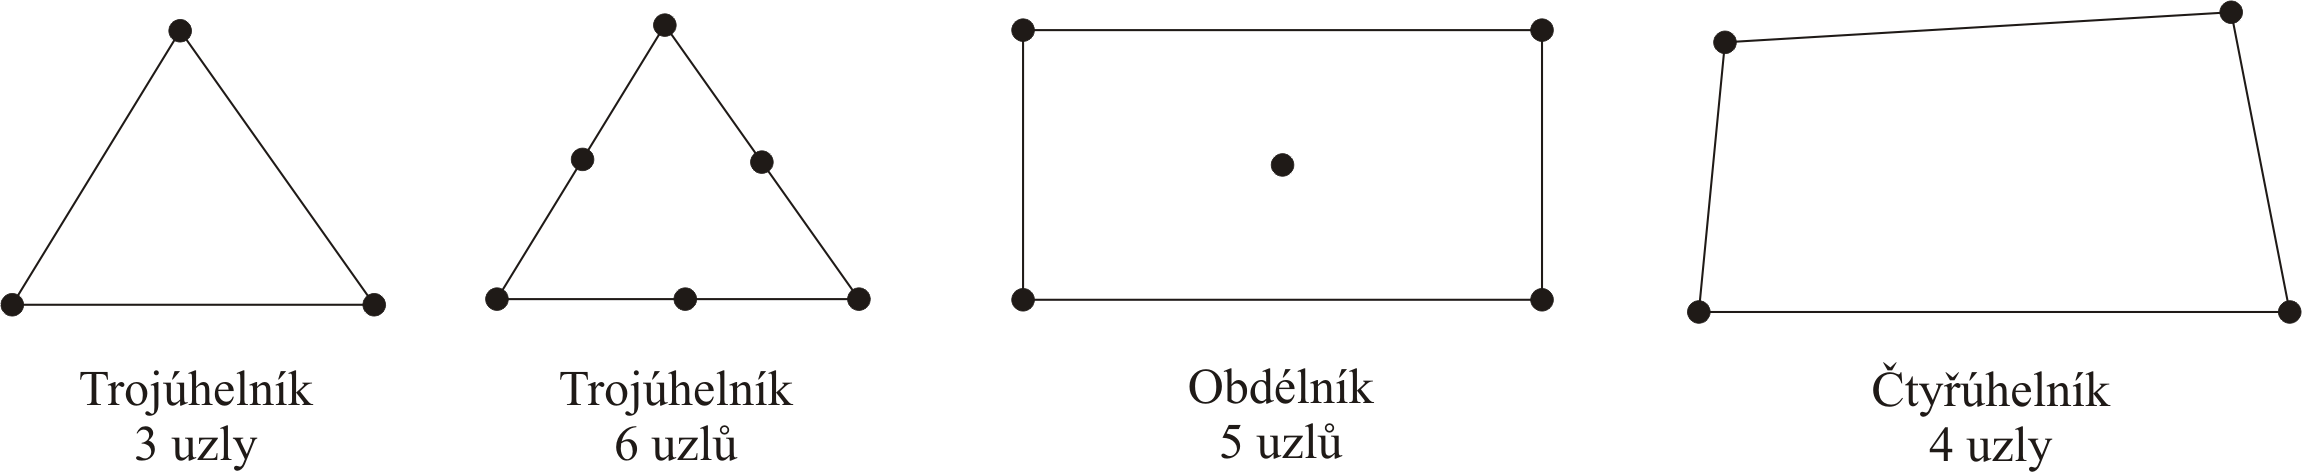
\includegraphics[width=9cm]{sim_prvky.png}
	\caption{Prvky diskterizace 2D oblasti. \cite{num}}
	\label{obr:sim_prvky}
\end{figure}

\subsection{Aproximované řešení}
Pro řešení diferenciální rovnice druhého řádu na obecné oblasti $\Omega$ je potřeba nejprve odvodit slabou formu. Ta představuje vynásobení rovnice testovací funkcí $v$ a poté integraci přes oblast řešení $\Omega$. Podrobný postup převodu pro Helmholtzovu rovnici (\ref{rce:sim_helmholtz_vychozi}) je blíže popsán v~podkapitole \ref{sec:sim_hermes2d}. Slabou formu výchozí řešené rovnice lze rozčlenit na bilineární a lineární členy. Bilineární člen $b(E_z,v)$ představuje levou stranu rovnic ve slabé formě a lineární člen $l(v)$ reprezentuje stranu pravou.
Aproximovaným řešením výchozí rovnice (\ref{rce:sim_kar_helmholtz_num}) je pak funkce $E_z$, pro kterou platí 
\begin{equation}
	b(E_z,v) = l(v),\qquad \mathrm{pro}\ E_z, v~\in V_{n}(\Omega),
	\label{rce:sim_aprox_reseni}
\end{equation}
kde $V_{n}(\Omega)$ představuje podprostor Hilbertova prostoru funkcí $H_{0}^{1}(\Omega)$. Řešení rovnice (\ref{rce:sim_aprox_reseni}) je možné zapsat jako lineární kombinaci bázových funkcí s~neznámými koeficienty, které je pro řešení potřeba nalézt
\begin{displaymath}
	E_z = \sum_{i=1}^{N}y_i v_i.
\end{displaymath}
Při položení bázových funkcí stejných jako testovací a dosazením do rovnice  (\ref{rce:sim_aprox_reseni}) obdržíme vztah
\begin{equation}
	\sum_{i=1}^{N}b(v_i,v_j)\cdot y_i = l(v_j),
	\label{rce:sim_aprox_reseni2}
\end{equation}
ze kterého vznikne systém algebraických rovnic s~neznámými koeficienty bázových funkcí, které aproximují řešení výchozí diferenciální rovnice na oblasti $\Omega$
\begin{equation}
	\vec S~\cdot \vec Y = \vec G.
	\label{rce:sim_aprox_matice}
\end{equation}
Matice $\vec S$ se označuje jako \uv{matice tuhosti}. Název má spojitost s~historií a pochází z~teorie elastických deformací. V~rovnici (\ref{rce:sim_aprox_matice}) je definována
\begin{displaymath}
	\vec S~= \{b(v_i,v_j) \}_{i,j = 1}^{N}.
\end{displaymath}
Vektor pravých stran lze zapsat
\begin{displaymath}
	\vec G = \{l(v_j) \}_{j = 1}^{N}
\end{displaymath}
a vektor neznámých koeficientů
\begin{displaymath}
	\vec Y = \{y_j \}_{j = 1}^{N}.
\end{displaymath}
Je zřejmé, že nalezení hledaných koeficientů $y_j$ spočívá v~řešení maticové rovnice ve tvaru
\begin{equation}
	\vec Y = \vec S~^{-1}\cdot \vec G.
	\label{rce:sim_aprox_inv_matice}
\end{equation}

\section{Řešení harmonické vlnové rovnice knihovnou Hermes2D} \label{sec:sim_hermes2d}
Vzhledem k~široké problematice elektromagnetických vln je potřeba pro jejich modelování zavést některé zjednodušení. 
\begin{itemize}
\item {\bf Harmonická analýza} - První předpokladem je řešení vlnové rovnice v~harmonickém tvaru (Helmholtzova rovnice)
\begin{equation}
	\nabla\times(\nabla\times\vecfaz E) +\faz k^{2}\vecfaz E = \mathrm{grad}\frac{\rho}{\varepsilon} + \mj\omega\mu\faz J_{\mathrm{ext}}.
    \label{rce:sim_helmholtz_vychozi} 
\end{equation}
\item {\bf Rovnoměrné rozložení náboje $\rho$} - Při této úvaze je v~řešené rovnici (\ref{rce:sim_helmholtz_vychozi}) člen $\mathrm{grad}\frac{\rho}{\varepsilon}$ roven nule.
\item {\bf Šíření vln v~kartézské souřadnicové soustavě v~jediném směru dle osy $z$} - Tento předpoklad platí pro planární problém.
\item {\bf Šíření vln v~polární souřadnicové soustavě má pouze tangenciální složku} - Uvažujeme pro osově symetrický problém.
\end{itemize}

\subsection{Kartézská souřadnicová soustava} \label{subsec:sim_kar}
Zavedením zjednodušujících předpokladů vycházíme z~rovnice ve tvaru
\begin{equation}
	\nabla^{2}\faz E_{(z)} +\faz k^{2}\faz E_{(z)} = \mj\omega\mu\faz J_{\mathrm{ext}},
	\label{rce:sim_kar_helmholtz_num} 
\end{equation}
platné na definované oblasti $\Omega$, na které známe okrajové podmínky a ve které chceme dostat výsledné řešení. Tím může být například vnitřní prostor vlnovodu nebo rezonátoru. Pro získání slabé formy k~rovnici (\ref{rce:sim_kar_helmholtz_num}) nejprve vyjádříme reálnou a imaginární složku
\begin{displaymath}
	\nabla^{2}(E_{z\Re} + \mj E_{z\Im}) + (\omega^{2}\varepsilon\mu - \mj\omega\mu\sigma)(E_{z\Re} + \mj E_{z\Im}) = \mj\omega\mu (J_{\mathrm{ext}\Re} + \mj J_{\mathrm{ext}\Im}),
\end{displaymath}
\begin{displaymath}
	\nabla^{2} E_{z\Re} + \mj\nabla^{2} E_{z\Im} + \omega^{2}\varepsilon\mu E_{z\Re} + \mj\omega^{2}\varepsilon\mu E_{z\Im} - \mj\omega\mu\sigma E_{z\Re} + \omega\mu\sigma E_{z\Im} = - \omega\mu J_{\mathrm{ext}\Im} + \mj\omega\mu J_{\mathrm{ext}\Re},
\end{displaymath}
kde reálnou část tvoří
\begin{equation}
	\Re : \nabla^{2} E_{z\Re} + \omega^{2}\varepsilon\mu E_{z\Re} + \omega\mu\sigma E_{z\Im} = - \omega\mu J_{\mathrm{ext}\Im}
	\label{rce:sim_kar_num_real} 
\end{equation}
a imaginární je vyjádřena
\begin{equation}
	\Im : \nabla^{2} E_{z\Im} + \omega^{2}\varepsilon\mu E_{z\Im} - \omega\mu\sigma E_{z\Re} = \omega\mu J_{\mathrm{ext}\Re}.
	\label{rce:sim_kar_num_imag} 
\end{equation}
Obě upravené rovnice (\ref{rce:sim_kar_num_real}) a (\ref{rce:sim_kar_num_imag}) je již možné převést do slabých forem, které splňují nulovou Dirichletovu a Neumannovu okrajovou podmínku. Postup převodu spočívá ve vynásobení parciálních diferenciálních rovnic testovací funkcí $v$ a v~následné integraci přes oblast řešení $\Omega$ 
\begin{equation}
	\Re : \int_{\Omega}\nabla^{2} E_{z\Re}\cdot v~\dif S~+ \omega^{2}\varepsilon\mu\int_{\Omega} E_{z\Re}\cdot v\dif S~+ \omega\mu\sigma\int_{\Omega} E_{z\Im}\cdot v\dif S~= - \omega\mu \int_{\Omega}J_{\mathrm{ext}\Im}\cdot v~\dif S,
	\label{rce:sim_kar_weak_odv_real} 
\end{equation}
\begin{equation}
	\Im : \int_{\Omega}\nabla^{2} E_{z\Im}\cdot v\dif S~+ \omega^{2}\varepsilon\mu\int_{\Omega} E_{z\Im}\cdot v\dif S~- \omega\mu\sigma\int_{\Omega} E_{z\Re}\cdot v\dif S~= \omega\mu \int_{\Omega}J_{\mathrm{ext}\Re}\cdot v~\dif S.
	\label{rce:sim_kar_weak_odv_imag} 
\end{equation}
V~dalším kroku se aplikuje 1. Greenova identita \cite[příloha A.2]{num} (integrace po částech pro vyšší řády) a tím se konečně získají slabé formy k~původním rovnicím (\ref{rce:sim_kar_num_real}) a (\ref{rce:sim_kar_num_imag})
\begin{displaymath}
\Re : \int_{\Gamma}\frac{\partial E_{z\Re}}{\partial n}\cdot v\dif l-\int_{\Omega}\nabla E_{z\Re}\cdot\nabla v~\dif S~+ \omega^{2}\varepsilon\mu\int_{\Omega} E_{z\Re}\cdot v\dif S~+ \omega\mu\sigma\int_{\Omega} E_{z\Im}\cdot v\dif
S~\end{displaymath}
\begin{equation}
	 = - \omega\mu \int_{\Omega}J_{\mathrm{ext}\Im}\cdot v~\dif S,
	\label{rce:sim_kar_weak_real} 
\end{equation}
\begin{displaymath}
\Im : \int_{\Gamma}\frac{\partial E_{z\Im}}{\partial n}\cdot v\dif l-\int_{\Omega}\nabla E_{z\Im}\cdot\nabla v\dif S~+ \omega^{2}\varepsilon\mu\int_{\Omega} E_{z\Im}\cdot v\dif S~- \omega\mu\sigma\int_{\Omega} E_{z\Re}\cdot v\dif S~\end{displaymath}
\begin{equation}
	= \omega\mu \int_{\Omega}J_{\mathrm{ext}\Re}\cdot v~\dif S.
	\label{rce:sim_kar_weak_imag} 
\end{equation}
První člen $\int_{\Gamma}\frac{\partial E_{z\Re}}{\partial n}\cdot v\dif l$ (respektive $\int_{\Gamma}\frac{\partial E_{z\Im}}{\partial n}\cdot v\dif l$) vyjadřuje Neumanovu okrajovou podmínku. Pokud je podmínka nulová, tak i tyto členy budou nulové. 

Levé strany rovnic představují bilineární členy daných slabých forem. Na pravých stranách se nacházejí členy lineární. K~první rovnici (\ref{rce:sim_kar_weak_real}) lze bilineární člen zapsat jako
\begin{equation}
	b(E_{z},v) = -\int_{\Omega}\nabla E_{z\Re}\cdot\nabla v~\dif S~+ \omega^{2}\varepsilon\mu\int_{\Omega} E_{z\Re}\cdot v\dif S~+ \omega\mu\sigma\int_{\Omega} E_{z\Im}\cdot v\dif
S~\label{rce:sim_kar_bilinear_real} 
\end{equation}
a lineární člen vztahem
\begin{equation}
	l(v) = - \omega\mu \int_{\Omega}J_{\mathrm{ext}\Im}\cdot v~\dif S.
	\label{rce:sim_kar_linear_real}
\end{equation}
U~rovnice druhé (\ref{rce:sim_kar_weak_imag}) jsou lineární a bilineární členy vyjádřeny
\begin{equation}
	b(E_{z},v) = -\int_{\Omega}\nabla E_{z\Im}\cdot\nabla v\dif S~+ \omega^{2}\varepsilon\mu\int_{\Omega} E_{z\Im}\cdot v\dif S~- \omega\mu\sigma\int_{\Omega} E_{z\Re}\cdot v\dif S,
	\label{rce:sim_kar_bilinear_imag}	
\end{equation}
\begin{equation}
	l(v) = \omega\mu \int_{\Omega}J_{\mathrm{ext}\Re}\cdot v~\dif S.
	\label{rce:sim_kar_linear_imag}
\end{equation}

\subsection{Polární souřadnicová soustava}
Řešení vlnové rovnice v~polárních souřadnicích vychází z~rovnice
\begin{equation}
	\nabla\times(\nabla\times\faz E_{\alpha}) +\faz k^{2}\faz E_{\alpha} = \mj\omega\mu\faz J_{\mathrm{ext}},
	\label{rce:sim_pol_helmholtz_num} 
\end{equation}
ve které je zavedeno zjednodušení, že výsledek má pouze tangenciální složku. Potom můžeme rovnici (\ref{rce:sim_pol_helmholtz_num}) snadno upravit. Nejprve vyjádříme vnitřní rotaci
\begin{displaymath}
	\nabla\times \frac{1}{r}\Bigg|
	\begin{array}{ccc}
\hat{r} & r\hat{\alpha} & \hat{z} \\
\frac{\partial}{\partial r} & \frac{\partial}{\partial \alpha} & \frac{\partial}{\partial z} \\
0 & r\faz E_{\alpha} & 0\\
\end{array}\Bigg| +\faz k^{2}\faz E_{\alpha} = \mj\omega\mu\faz J_{\mathrm{ext}},
\end{displaymath}
\begin{equation}
\nabla\times \Bigg[\hat{r}\bigg(-\frac{1}{r}\cdot\frac{\partial r\faz E_{\alpha}}{\partial z}\bigg) + \hat{\alpha}\bigg(0\bigg) + \hat{z}\bigg(\frac{1}{r}\cdot\frac{\partial r\faz E_{\alpha}}{\partial r}\bigg) \Bigg]+\faz k^{2}\faz E_{\alpha} = \mj\omega\mu\faz J_{\mathrm{ext}}.
	\label{rce:sim_pol_rotace1}
\end{equation}
Analogickým způsobem upravíme vnější rotaci ve vztahu (\ref{rce:sim_pol_rotace1})
\begin{displaymath}
	\frac{1}{r}\Bigg|
	\begin{array}{ccc}
\hat{r} & r\hat{\alpha} & \hat{z} \\
\frac{\partial}{\partial r} & \frac{\partial}{\partial \alpha} & \frac{\partial}{\partial z} \\
-\frac{1}{r}\cdot\frac{\partial r\faz E_{\alpha}}{\partial z} & 0 & \frac{1}{r}\cdot\frac{\partial r\faz E_{\alpha}}{\partial r}\\
\end{array}\Bigg| +\faz k^{2}\faz E_{\alpha} = \mj\omega\mu\faz J_{\mathrm{ext}},
\end{displaymath}
\begin{equation}
\Bigg[\hat{r}\bigg(\frac{1}{r}\cdot\frac{\partial}{\partial \alpha}\cdot\frac{1}{r}\frac{\partial r\faz E_{\alpha}}{\partial r}\bigg) + \hat{\alpha}\bigg(-\frac{\partial}{\partial z}\cdot\frac{1}{r}\cdot\frac{\partial r\faz E_{\alpha}}{\partial z} - \frac{\partial}{\partial r}\cdot\frac{1}{r}\cdot\frac{\partial r\faz E_{\alpha}}{\partial r}\bigg) + \hat{z}\bigg(\frac{1}{r}\cdot\frac{\partial}{\partial \alpha}\cdot\frac{1}{r}\frac{\partial r E_{\alpha}}{\partial z}\bigg) \Bigg]+\faz k^{2}\faz E_{\alpha} = \mj\omega\mu\faz J_{\mathrm{ext}}.
	\label{rce:sim_pol_rotace2}
\end{equation}
Ve výsledném vztahu (\ref{rce:sim_pol_rotace2}) zanedbáme všechny ostatní složky kromě té, která respektuje souřadnici $\hat{\alpha}$. Dostaneme rovnici
\begin{displaymath}
-\frac{\partial}{\partial z}\cdot\frac{1}{r}\cdot\frac{\partial r\faz E_{\alpha}}{\partial z} - \frac{\partial}{\partial r}\cdot\frac{1}{r}\cdot\frac{\partial r\faz E_{\alpha}}{\partial r}+\faz k^{2}\faz E_{\alpha} = \mj\omega\mu\faz J_{\mathrm{ext}},
\end{displaymath}
kterou upravíme do podoby
\begin{equation}
-\frac{\partial^{2}E_{\alpha}}{\partial z^{2}}-\frac{\partial^{2}E_{\alpha}}{\partial r^{2}}-\frac{1}{r}\cdot\frac{\partial E_{\alpha}}{\partial r} + \frac{E_{\alpha}}{r^{2}} +\faz k^{2}\faz E_{\alpha} = \mj\omega\mu\faz J_{\mathrm{ext}}.
	\label{rce:sim_pol_helmholtz_upravena}
\end{equation}
Tento vztah představuje vyjádření Helmholtzovy rovnice v~polárních souřadnicích, při uvažování výše uvedených předpokladů simulace. Pro zápis programového kódu k~vyřešení rozložení pole při osové symetrii je potřeba, stejným způsobem jako v~části \ref{subsec:sim_kar}, odvodit slabou formu k~rovnici (\ref{rce:sim_pol_helmholtz_upravena}) 
splňující Dirichletovu i Neumannovu okrajovou podmínku. 

\section{Okrajové podmínky}
Pro řešení diferenciálních rovnic popisující chování elektromagnetického pole v~dané oblasti $\Omega$ je třeba znát okrajové podmínky na hranicích. Účelem je specifikovat chování výsledné funkce, případně derivace této funkce, v~daných bodech ležících na okraji řešené oblasti. Při popisu fyzikálních polí pomocí diferenciálních rovnic se užívá Dirichletova, Neumannova nebo Newtonova (smíšená) okrajová podmínka.
\begin{itemize}
\item {\bf Dirichletova okrajová podmínka} - Předepisuje na hranici $\Gamma$ hodnotu funkce $E_{(z)}$, která může být obecně závislá na čase nebo na souřadnicích
\begin{displaymath}
	\faz E_{(z)}|_{\Gamma} = f_{Dir}(x,y,z,t). 
\end{displaymath}
\item {\bf Neumannova okrajová podmínka} - Na okraji řešené oblasti definuje tato podmínka hodnotu normálové derivace funkce $\frac{\partial E_{(z)}}{\partial n}$
\begin{displaymath}
	\frac{\partial \faz E_{(z)}}{\partial n}|_{\Gamma} = f_{Neu}(x,y,z,t). 
\end{displaymath}
\item {\bf Newtonova okrajová podmínka} - Neboli smíšená podmínka, kombinuje obě předchozí uvedené. Na hranici $\Gamma$ tak specifikuje kombinaci hodnoty funkce $E_{(z)}$ a její normálové derivace $\frac{\partial E_{(z)}}{\partial n}$
\begin{displaymath}
	\bigg(\frac{\partial \faz E_{(z)}}{\partial n} + \faz E_{(z)}\bigg)|_{\Gamma} = f_{New}(x,y,z,t). 
\end{displaymath}
\end{itemize}

\section{Možnosti zobrazení výsledků řešení}
Vlastnosti postprocessingu zobrazení v~programu Agors2D jsou velmi obsáhlé. Pomocí levého panelu v~pracovním okně (patrné na obrázku \ref{obr:sim_agros2d}) je možné vybrat zobrazení ve 2D nebo 3D prostoru a řadu dalších vlastností. 

Příslušné vztahy pro interpretaci výsledků je však potřeba implemetovat v~samostatném modulu, patřící k~jednotlivým polím. V~případě elektromagnetického pole nás bude zajímat především rozložení intenzit elektrického a magnetického pole, magnetické indukce, Poyntingova vektoru a ztrát. Programové kódy pro všechny zmíněné veličiny pole v~kartézských souřadnicích se nachází v~příloze \ref{kap:Program_kod}. 
 
\subsection*{Intenzita elektrického pole}
Hodnoty této veličiny v~řešených v~bodech na oblasti $\Omega$ odpovídají přímo řešení rovnice (\ref{rce:sim_kar_helmholtz_num}) v~kartézských souřadnicích nebo rovnice (\ref{rce:sim_pol_helmholtz_num}) v~polární souřadnicové soustavě.

\subsection*{Magnetická indukce}
Odvození vztahů pro zobrazení magnetické indukce vychází z~druhého Maxwellova zákona (\ref{rce:1MaxwR}), který má pro harmonické pole tvar
\begin{displaymath}
	\rot\vecfaz E = -\mj\omega\vecfaz B.
\end{displaymath}
Po úpravě rotace na levé straně výrazu pro jedinou složku $E_z$ dostaneme vztah
\begin{equation}
	\frac{\partial \faz E_z}{\partial y}\cdot\overrightarrow{\mathrm{i}} - \frac{\partial \faz E_z}{\partial y}\cdot\overrightarrow{\mathrm{j}} + 0\cdot\overrightarrow{\mathrm{k}} = -\mj\omega \faz B_x\cdot\overrightarrow{\mathrm{i}} - \mj\omega\faz  B_y\cdot\overrightarrow{\mathrm{j}} - \mj\omega\faz B_z\cdot\overrightarrow{\mathrm{k}},
	\label{rce:sim_zobrazeni_flux}
\end{equation}
ze kterého lze vyjádřit $x$-ová a $y$-ová složka magnetické indukce. $\faz B_z$ je podle rovnice (\ref{rce:sim_zobrazeni_flux}) nulová. Pro $\faz B_x$ tedy platí
\begin{displaymath}
	\faz B_x = -\frac{1}{\mj\omega}\frac{\partial E_z}{\partial y},
\end{displaymath}
kde po dosazení za $\faz E_z$ můžeme vyjádřit reálnou a imaginární složku magnetické indukce ve směru $x$, které lze pak implemetovat do modulu
\begin{equation}
	B_{x\Re} = -\frac{1}{\mj\omega}\frac{\partial E_{z\Im}}{\partial y}, \qquad \qquad B_{x\Im} = \frac{1}{\mj\omega}\frac{\partial E_{z\Re}}{\partial y}.
	\label{rce:sim_flux_x_re}
\end{equation}
Z~rovnice (\ref{rce:sim_zobrazeni_flux}) je pak dále možné stejným způsobem odvodit vztahy pro obě složky indukce ve směru $y$
\begin{equation}
	B_{y\Re} = \frac{1}{\mj\omega}\frac{\partial E_{z\Im}}{\partial x}, \qquad \qquad B_{y\Im} = -\frac{1}{\mj\omega}\frac{\partial E_{z\Re}}{\partial x}.
	\label{rce:sim_flux_y_im}
\end{equation}
Nakonec zbývá vyjádřit rozložení modulu magnetické indukce. Pro jeho velikost platí
\begin{displaymath}
	B = \sqrt{B_{x}^{2} + B_{y}^{2}} = \sqrt{B_{x\Re}^{2} + B_{x\Im}^{2} + B_{y\Re}^{2} + B_{y\Im}^{2}}.
\end{displaymath}

\subsection*{Intenzita magnetické pole}
Vztahy pro zobrazení magnetické složky pole s~výhodou vycházejí již z~vyjádřené magnetické indukce, neboť v harmonickém poli platí
\begin{displaymath}
\vecfaz H = \frac{1}{\mu} \vecfaz B.
\end{displaymath}
Je zřejmé, že veškeré výše odvozené vztahy (\ref{rce:sim_flux_x_re}) až (\ref{rce:sim_flux_y_im}) lze pouze podělit hodnotou permeability, která se nachází v~řešené oblasti. 

\subsection*{Poyntingův vektor}
Vektor vyjádřený vektorovým součinem intenzit elektrického a magnetického pole představuje plošnou hustotu výkonu na řešené oblasti $\Omega$
\begin{equation}
	\vecfaz N = \vecfaz E \times\vecfaz H\unit{[W/m^{2}]}.
	\label{rce:sim_poynting_vec}
\end{equation}
Úpravou rovnice (\ref{rce:sim_poynting_vec}) dostaneme vyjádření pro rozložení jednotlivé složky Poyntingova vektoru
\begin{equation}
	\faz N_x \cdot\overrightarrow{\mathrm{i}} + \faz N_y \cdot\overrightarrow{\mathrm{j}} + \faz N_z \cdot\overrightarrow{\mathrm{k}} = (-\faz E_z \faz H_y) \cdot\overrightarrow{\mathrm{i}} + \faz E_z \faz H_x \cdot\overrightarrow{\mathrm{j}} + 0 \cdot\overrightarrow{\mathrm{k}}.
	\label{rce:sim_poynting_vec_rozepsany}
\end{equation}
Je zřejmé, že $N_z$ je dle výrazu (\ref{rce:sim_poynting_vec_rozepsany}) nulový. Pro $x$-ovou složku platí
\begin{displaymath}
	\faz N_x = -\faz E_z \faz H_y,
\end{displaymath}
\begin{displaymath}
	\faz N_x = -(E_{z\Re} + \mj E_{z\Im})\cdot (H_{y\Re} + \mj H_{y\Im}),
\end{displaymath}
což ve výsledku vede na vztah
\begin{displaymath}
	\faz N_x = E_{z\Im} H_{y\Im} - E_{z\Re} H_{y\Re} - \mj (E_{z\Re} H_{y\Im} + E_{z\Im} H_{y\Re}).
\end{displaymath}
Pro Poyntingův vektor ve směru $y$ analogicky vychází
\begin{displaymath}
	\faz N_y = \faz E_z \faz H_x,
\end{displaymath}
\begin{displaymath}
	\faz N_y = E_{z\Re} H_{x\Re} - E_{z\Im} H_{x\Im} + \mj (E_{z\Re} H_{x\Im} + E_{z\Im} H_{x\Re}).
\end{displaymath}
Pro výslednou hodnotu Poyntingova vektoru na řešené oblasti $\Omega$ platí
\begin{displaymath}
	N = \sqrt{N_{x}^{2} + N_{y}^{2}} = \sqrt{(E_{z\Im} H_{y\Im} - E_{z\Re} H_{y\Re})^{2} + (E_{z\Im} H_{x\Im} - E_{z\Re} H_{x\Re})^{2}}.
\end{displaymath}

\subsection*{Jouleovy ztráty}
Rozložení ztrát v~řešené oblasti odpovídá součinu proudové hustoty $J$ a hodnoty intenzity elektrického pole $E$ 
\begin{displaymath}
	P_j = \faz J \cdot \faz E = \sigma \faz E^{2} = \sigma \sqrt{E_{z\Re}^{2} + E_{z\Im}^{2}}\unit{[J/m^{3}]}.
\end{displaymath}

\section{Numerická integrace}
Výpočet určitých integrálů, které se v~řešených vztazích vyskytují, je analyticky možný pouze v~určitých jednoduchých případech. Pro obecné funkce se integrace provádí numericky. Jednou z~možností je výpočet pomocí Gaussovy kvadratury.

Účelem je vypočítat numericky hodnodutu integrálu obecné funkce $g(\xi)$ na intervalu $x\in\langle a, b\rangle$,  pomocí aproximace výrazem
\begin{displaymath}
\sum_{i=0}^{n}\mathrm{w}_{t}[i]f(x_{i}),
\end{displaymath}
který se nazývá kvadraturní formule. Číslo $n$ představuje počet integračních bodů, hodnoty $\mathrm{w}_{t}[i]$ jsou příslušné váhové koeficienty uvedeného kvadraturního vzorce a $x_{i}$ se nazývají jeho uzly. 

Při výpočtu integrálu pomocí kvadraturní formule záleží tedy na volbě dělících bodů $x_{i}$ i koeficientů $\mathrm{w}_{t}[i]$. Právě princip Gaussovy kvadratury spočívá v~tom, jak vhodně zvolit $x_{i}$ a následně dopočítat $\mathrm{w}_{t}[i]$. Hodnoty uzlových bodů se pro jednorozměrný případ volí jako kořeny Legendrových polynomů
\begin{displaymath}
	P_{n}(x) = \frac{1}{2^{n}\cdot n!}\frac{\dif^{n}}{\dif x^{n}}[(x^{2} - 1)^{n}]
\end{displaymath}
a koeficienty $\mathrm{w}_{t}[i]$ jsou definovány
\begin{displaymath}
\mathrm{w}_{t}[i] = \frac{-2}{(n+2)P_{n+2}(x_i)P'_{n+1}(x_i)}.
\end{displaymath}
Více o~této metodě Gaussovy kvadratury je možné zjistit v~\cite{gk_tichy} nebo v~\cite{gk_kaw}.

\subsection{Numerický zápis rovnic kartézské souřadnicové soustavy}
\subsubsection*{Vyjádření členů rovnice (\ref{rce:sim_kar_weak_real})}
Bilineární člen rovnice, tj. vztah (\ref{rce:sim_kar_bilinear_real}) se ještě rozdělí na část reprezentovanou reálnou a imaginární složkou. Nejprve vyjádříme zápis, který je v~programu označen indexem \uv{real\_real}. Rozepsáním operátoru $\nabla$ a numerickým řešením integrálů obdržíme výraz
\begin{equation}
	-\sum_{i=0}^{n}\mathrm{w}_{t}[i]\bigg(\frac{\partial E_{z\Re}}{\partial x}\cdot \frac{\partial v}{\partial x} + \frac{\partial E_{z\Re}}{\partial y}\cdot \frac{\partial v}{\partial y} \bigg) + \omega^{2}\varepsilon\mu\sum_{i=0}^{n}\mathrm{w}_{t}[i]\bigg(E_{z\Re}\cdot v\bigg).
	\label{rce:sim_kar_weak_real_real_num} 
\end{equation}
Podobným způsobem postupujeme u~druhé složky bilineární části vyjádřené pomocí $E_{z\Im}$. Index funkce v~programu se změní na \uv{real\_imag}
\begin{equation}
 \omega\mu\sigma\sum_{i=0}^{n}\mathrm{w}_{t}[i]\bigg(E_{z\Im}\cdot v\bigg).
	\label{rce:sim_kar_weak_real_imag_num} 
\end{equation}
Nakonec je potřeba vyčíslit lineární část reálné složky, kterou reprezentuje rovnice (\ref{rce:sim_kar_linear_real})
\begin{equation}
 -\omega\mu\sum_{i=0}^{n}\mathrm{w}_{t}[i]\bigg(J_{\mathrm{ext}\Im}\cdot v\bigg).
	\label{rce:sim_kar_linear_real_num} 
\end{equation}


\subsubsection*{Členy rovnice (\ref{rce:sim_kar_weak_imag})}
Postup je naprosto totožný jako u~slabé formy reálné složky výchozí rovnice. Tudíž opět rozdělíme bilineární část na dvě části dle $E_{z\Re}$ a $E_{z\Im}$. Pro bilineární část (\ref{rce:sim_kar_bilinear_imag}) související s~indexem \uv{imag\_real} platí
\begin{equation}
 -\omega\mu\sigma\sum_{i=0}^{n}\mathrm{w}_{t}[i]\bigg(E_{z\Im}\cdot v\bigg)
	\label{rce:sim_kar_weak_imag_real_num} 
\end{equation}
a označení \uv{imag\_imag} odpovídá
\begin{equation}
	-\sum_{i=0}^{n}\mathrm{w}_{t}[i]\bigg(\frac{\partial E_{z\Im}}{\partial x}\cdot \frac{\partial v}{\partial x} + \frac{\partial E_{z\Im}}{\partial y}\cdot \frac{\partial v}{\partial y} \bigg) + \omega^{2}\varepsilon\mu\sum_{i=0}^{n}\mathrm{w}_{t}[i]\bigg(E_{z\Im}\cdot v\bigg).
	\label{rce:sim_kar_weak_imag_imag_num} 
\end{equation}
Imaginární lineární část (\ref{rce:sim_kar_linear_imag}) je reprezentovaná zápisem
\begin{equation}
 \omega\mu\sum_{i=0}^{n}\mathrm{w}_{t}[i]\bigg(J_{\mathrm{ext}\Re}\cdot v\bigg).
	\label{rce:sim_kar_linear_imag_num} 
\end{equation}

\subsection{Numerický zápis rovnic polární souřadnicové soustavy}
\subsubsection*{Reálná část vztahu (\ref{rce:sim_pol_helmholtz_upravena})}
Bilineární člen dané slabé formy s~indexem \uv{real\_real} lze po zavedení numerické integrace zapsat jako
\begin{displaymath}
-\sum_{i=0}^{n}\mathrm{w}_{t}[i]\bigg(\frac{\partial E_{\alpha\Re}}{\partial z}\cdot \frac{\partial v}{\partial z} + \frac{\partial E_{\alpha\Re}}{\partial r}\cdot \frac{\partial v}{\partial r} \bigg) - \frac{1}{r}\sum_{i=0}^{n}\mathrm{w}_{t}[i]\bigg(\frac{\partial E_{\alpha\Re}}{\partial r}\cdot v\bigg) +
\end{displaymath}
\begin{equation}
	 + \frac{1}{r^{2}}\sum_{i=0}^{n}\mathrm{w}_{t}[i]\bigg(E_{\alpha\Re}\cdot v\bigg) + \omega^{2}\varepsilon\mu\sum_{i=0}^{n}\mathrm{w}_{t}[i]\bigg(E_{\alpha\Re}\cdot v\bigg).
	\label{rce:sim_pol_bilinear_real_real} 
\end{equation}
Je zřejmé, že forma označená \uv{real\_imag} vyjde identicky jako v~případě kartézské souřadnicové soustavy, neboť člen $+\faz k^{2}\faz E_{\alpha}$ v~rovnici (\ref{rce:sim_pol_helmholtz_upravena}) je formálně stejný se vztahem (\ref{rce:sim_kar_helmholtz_num}). Platí tedy
\begin{equation}
 \omega\mu\sigma\sum_{i=0}^{n}\mathrm{w}_{t}[i]\bigg(E_{\alpha\Im}\cdot v\bigg).
	\label{rce:sim_pol_bilinear_real_imag} 
\end{equation}
Nakonec je potřeba zapsat lineární část reálné složky, která vyjde také identicky jako u~kartézské souřadnicové soustavy
\begin{equation}
 -\omega\mu\sum_{i=0}^{n}\mathrm{w}_{t}[i]\bigg(J_{\mathrm{ext}\Im}\cdot v\bigg).
	\label{rce:sim_pol_linear_real_num} 
\end{equation}

\subsubsection*{Imaginární část výrazu (\ref{rce:sim_pol_helmholtz_upravena})}
Slabým formám vycházející z~imaginární části z~původní rovnice (\ref{rce:sim_pol_helmholtz_upravena}) odpovídá vyjádření
\begin{equation}
 -\omega\mu\sigma\sum_{i=0}^{n}\mathrm{w}_{t}[i]\bigg(E_{\alpha\Re}\cdot v\bigg),
	\label{rce:sim_pol_bilinear_imag_real} 
\end{equation}
pro \uv{imag\_real}, což je opět ze stejného důvodu identické s~kartézskou souřadnicovou soustvou. Nakonec indexu \uv{imag\_imag} odpovídá
\begin{displaymath}
-\sum_{i=0}^{n}\mathrm{w}_{t}[i]\bigg(\frac{\partial E_{\alpha\Im}}{\partial z}\cdot \frac{\partial v}{\partial z} + \frac{\partial E_{\alpha\Im}}{\partial r}\cdot \frac{\partial v}{\partial r} \bigg) - \frac{1}{r}\sum_{i=0}^{n}\mathrm{w}_{t}[i]\bigg(\frac{\partial E_{\alpha\Im}}{\partial r}\cdot v\bigg) +
\end{displaymath}
\begin{equation}
	 + \frac{1}{r^{2}}\sum_{i=0}^{n}\mathrm{w}_{t}[i]\bigg(E_{\alpha\Im}\cdot v\bigg) + \omega^{2}\varepsilon\mu\sum_{i=0}^{n}\mathrm{w}_{t}[i]\bigg(E_{\alpha\Im}\cdot v\bigg).
	\label{rce:sim_pol_bilinear_imag_imag} 
\end{equation}
Imaginární lineární část je reprezentovaná opět identickým zápisem
\begin{equation}
 \omega\mu\sum_{i=0}^{n}\mathrm{w}_{t}[i]\bigg(J_{\mathrm{ext}\Re}\cdot v\bigg).
	\label{rce:sim_pol_linear_imag_num} 
\end{equation}

%\chapter{Závěr} \label{kap:Zaver}
%% !TeX root = Main.tex

Hlavním posláním této diplomové práce bylo vytvořit prostředek, pomocí kterého by bylo možné simulovat rozložení elektromagnetického pole při znalosti materiálových parametrů v~řešené oblasti a okrajových podmínek. Pro numerické řešení harmonické vlnové rovnice byla využita knihova Hermes2D, založená na metodě konečných prvků vyšších řádů přesnosti.

Celý simulační kód byl koncipován jako modul pro multiplatformní aplikaci Agros2D.  


Možnosti simulačního modulu byly demonstrovány na příkladu řešení vlnovodu R100 v~kapitole \ref{kap:Priklad}. Ověření výsledků bylo provedeno na stejném příkladu pomocí profesionálního programu COMSOL. Z~porovnání výsledků je patrné, že rozložení elektromagnetického pole je u~obou aplikací téměř identické. Drobné odlišnosti jsou způsobeny především přesností numerického řešení, která je závislá na míře diskretizace řešené oblasti ($h$-FEM) a řádu polynomu použitých prvků ($p$-FEM).

Příslušné parciální diferenciální rovnice byly odvozeny z~Maxwellových rovnic.



%% !TeX root = Main.tex

%\bibliography{references}
\bibliographystyle{plain}

\begin{thebibliography}{9}
\bibitem{emp}
{\sc Novotný, K.:}  {\bf Elektromagnetické pole a vlny: teorie elektromagnetického pole II},
Vydavatelství ČVUT, Praha~2001, \mbox{ISBN 80-01-02429-6}

\bibitem{hpfem}
{\em Oficiální internetové stránky sdružení hpFEM},
citováno dne \today \\
\texttt{http://www.hpfem.org/}

\bibitem{emc_trakce}
{\sc Kůs, V., Skála, J., Laurenc, J.:}  {\bf Elektrická trakce a EMC},
odborný článek, Plzeň~1997

\bibitem{nfr}
{\sc Kůs, K.:}  {\bf Nízkofrekvenční rušení},
skriptum, Západočeská univerzita, Plzeň~2003, \mbox{ISBN 80-7082-976-1}

\end{thebibliography}

%\newpage


%\listoffigures
%\listoftables
%\newpage

\appendix
%% !TeX root = Main.tex

\chapter{Odvození vlnových rovnic} \label{kap:Odvozeni_VlnR}
\section{Obecně časově proměnné pole} \label{sec:Odvozeni_CasPole}
K~sestavení vlnové diferenciální rovnice pro vektor intenzity elektrického pole $\vec E$ nebo vektor indukce magnetického pole $\vec B$ využijeme diferenciální tvar Maxwellových rovnic. 
\subsection*{Maxwellovy rovnice v~diferenciálním tvaru}
\begin{equation}
	\rot\vec H = \vec J+\frac{\partial\vec D}{\partial t}
	\label{rce:1MaxwR}
\end{equation}
\begin{equation}
	\rot\vec E = -\frac{\partial\vec B}{\partial t}
	\label{rce:2MaxwR}
\end{equation}
\begin{equation}
	\div\vec D = \rho
	\label{rce:3MaxwR}
\end{equation}
\begin{equation}
	\div\vec B = 0
	\label{rce:4MaxwR}
\end{equation}

\subsection{Vlnová rovnice pro vektor intenzity elektrického pole $\vec E$}
Dle \cite[str. 33]{emp} uvažujeme případ, že se v~daném objemu nachází indukovaný proud a~navíc proud, který vnucen vnějším zdrojem. Důsledkem je modifikace rovnice (\ref{rce:1MaxwR}).
\begin{equation}
	\rot\vec H = \vec J+\frac{\partial\vec D}{\partial t}+\vec J_{\mathrm{vn}}
	\label{rce:1MaxwR_vn}
\end{equation}
\begin{figure}[!h]
	\centering
	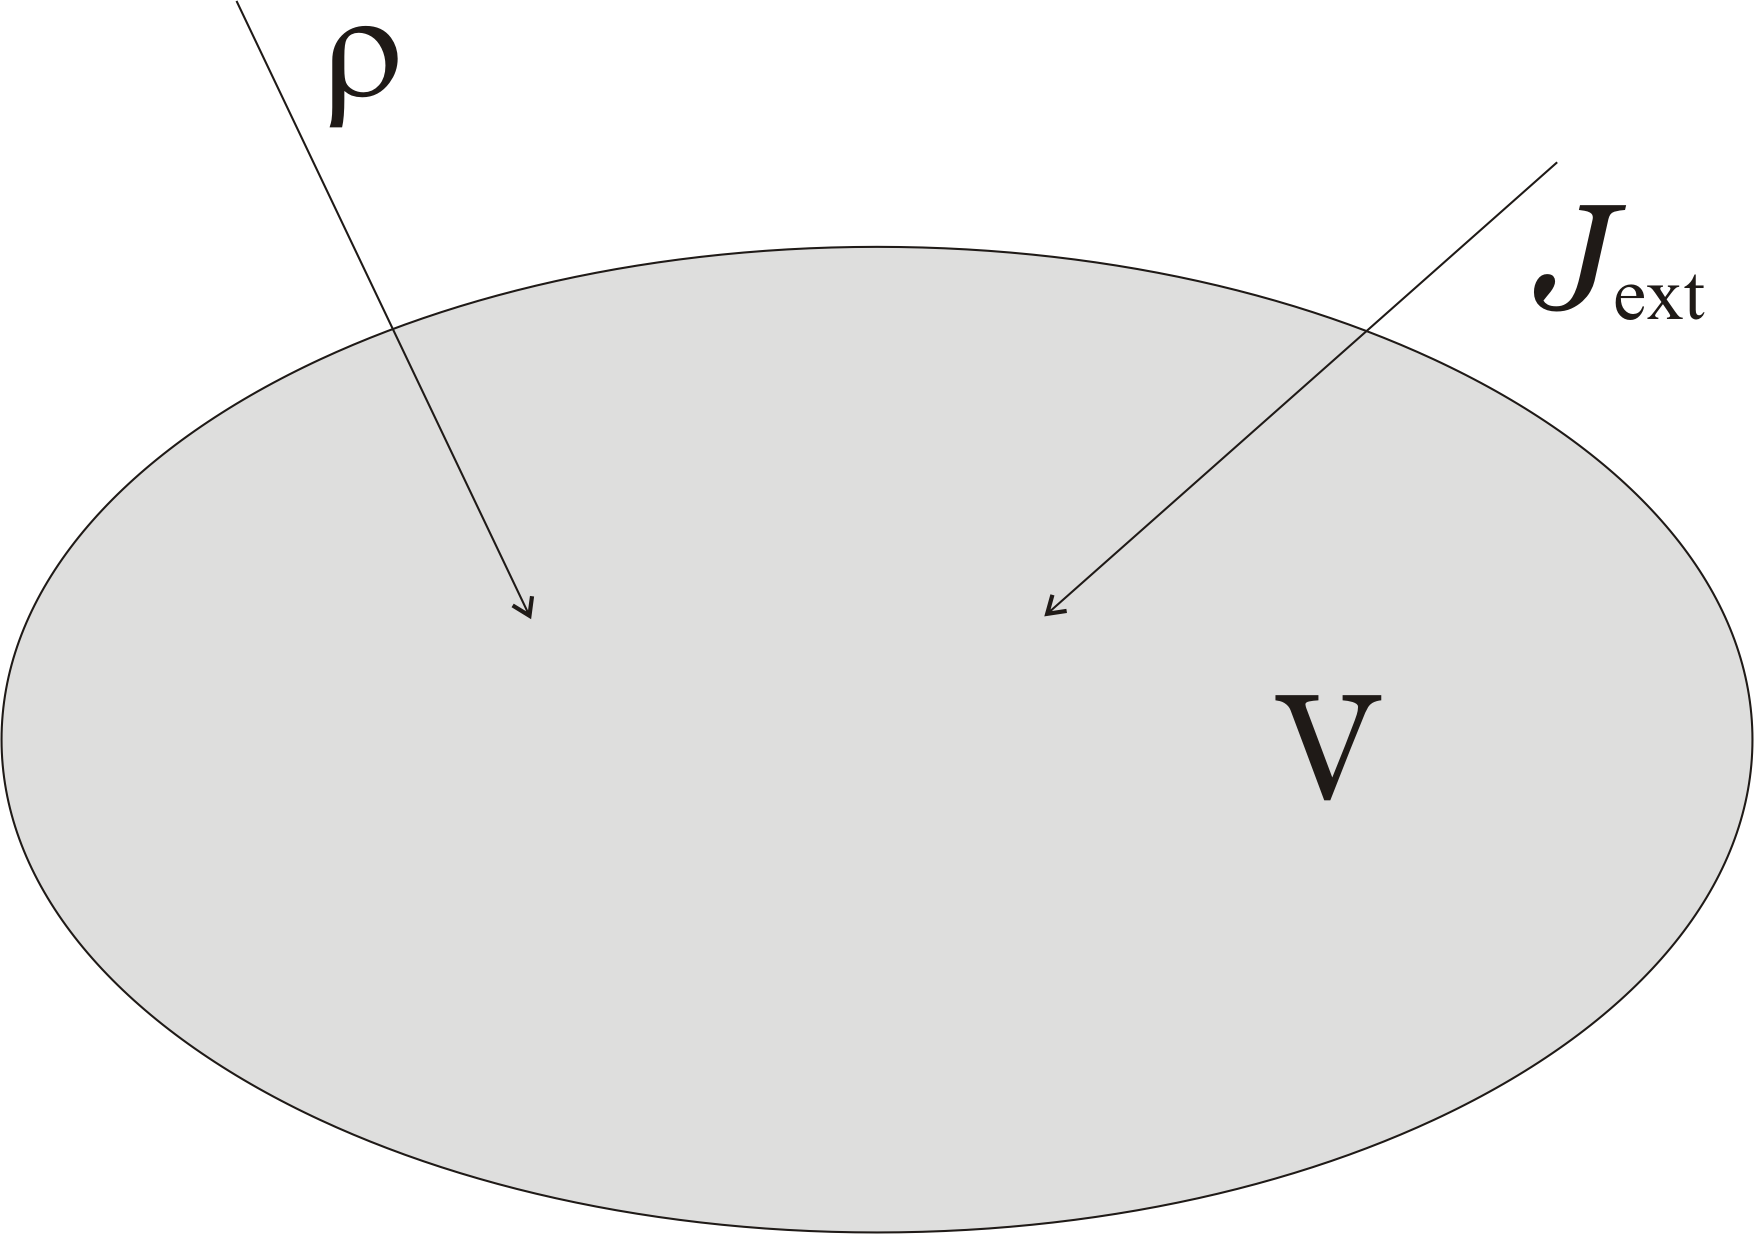
\includegraphics[width=4.5cm]{vnuceny_I.png}
	\caption{Vnucený proud vnějším zdrojem.}
	\label{obr:vnuceny_I}
\end{figure}\\
Vyjádření $\rot\vec B$ z~rovnice (\ref{rce:1MaxwR_vn}).
\begin{displaymath}
	\frac{1}{\mu} \rot\vec B = \sigma \vec E+\varepsilon\frac{\partial\vec E}{\partial t}+\vec J_{\mathrm{vn}}
\end{displaymath}
\begin{equation}
	\rot\vec B = \mu\sigma\vec E+\mu\varepsilon\frac{\partial\vec E}{\partial t}+\mu\vec J_{\mathrm{vn}}
	\label{rce:VlnR_ElPole_odv1}
\end{equation}
Na druhou Maxwelovu rovnici (\ref{rce:2MaxwR}) aplikujeme operaci rotace.
\begin{displaymath}
	\rot\rot\vec E = -\frac{\partial}{\partial t}\rot\vec B
\end{displaymath}
Za výraz $\rot\vec B$ na pravé straně rovnice dosadíme z~(\ref{rce:VlnR_ElPole_odv1}).
\begin{displaymath}
	\rot\rot\vec E = -\frac{\partial}{\partial t}\Big(\mu\sigma\vec E+\mu\varepsilon\frac{\partial\vec E}{\partial t}+\mu\vec J_{\mathrm{vn}}\Big)
\end{displaymath}
Pravou stranu rovnice roznásobíme a na levou použijeme vztah vektorové identity $\rot\rot\vec E = \grad\div\vec E - \nabla^{2}\vec E$. 
\begin{displaymath}
	\grad\div\vec E - \nabla^{2}\vec E = -\mu\sigma\frac{\partial\vec E}{\partial t}-\mu\varepsilon\frac{\partial^{2}\vec E}{\partial t^{2}}-\mu\frac{\partial\vec J_{\mathrm{vn}}}{\partial t}
\end{displaymath}
Ze třetí Maxwellovy rovnice (\ref{rce:3MaxwR}) dosadíme za $\div\vec E$ výraz $\frac{\rho}{\varepsilon}$. Úpravou přesuneme na~pravou stranu zdrojové funkce elektromagnetického pole a dostaneme výslednou vlnovou rovnici pro vektor intenzity elektrického pole $\vec E$.
\begin{equation}
	\nabla^{2}\vec E -\mu\sigma\frac{\partial\vec E}{\partial t}-\mu\varepsilon\frac{\partial^{2}\vec E}{\partial t^{2}} = \grad\frac{\rho}{\varepsilon}+\mu\frac{\partial\vec J_{\mathrm{vn}}}{\partial t}
	\label{rce:VlnR_ElPole}
\end{equation}
Rovnice (\ref{rce:VlnR_ElPole}) je dle \cite{emp} označována jako {\bf zobecněná nehomogenní vlnová rovnice}. Pro oblast bez vnějších zdrojů 
odpovídá $\rho = 0$ a $\vec J_{\mathrm{vn}} = 0$. Zavedení této úpravy získáme {\bf zobecněnou homogenní vlnovou rovnici} (\ref{rce:VlnR_ElPole_BezZdroju}).
\begin{equation}
	\nabla^{2}\vec E -\mu\sigma\frac{\partial\vec E}{\partial t}-\mu\varepsilon\frac{\partial^{2}\vec E}{\partial t^{2}} = 0
	\label{rce:VlnR_ElPole_BezZdroju}
\end{equation}

\subsection{Vlnová rovnice pro vektor indukce magnetického pole $\vec B$}
Vycházíme ze stejné počáteční úvahy jako při odvození vlnové rovnice pro vektor elektrické intenzity $\vec E$. Z~modifikované první Maxwellovy rovnice (\ref{rce:1MaxwR_vn}) opět vyjádříme $\rot \vec B$. Následně aplikujeme operaci rotace.
\begin{displaymath}
	\rot\vec B = \mu\sigma\vec E+\mu\varepsilon\frac{\partial\vec E}{\partial t}+\mu\vec J_{\mathrm{vn}}
\end{displaymath}
\begin{displaymath}
	\rot\rot\vec B = \mu\sigma\rot\vec E+\mu\varepsilon\frac{\partial \rot\vec E}{\partial t}+\mu\,\rot\vec J_{\mathrm{vn}}
\end{displaymath}
Na levou stranu použijeme vztah vektorové identity $\rot\rot\vec B = \grad\div\vec B - \nabla^{2}\vec B$. Za výraz $\rot \vec E$ dosadíme z~druhé Maxwellovy rovnice (\ref{rce:2MaxwR}). 
\begin{displaymath}
	\grad\div\vec B - \nabla^{2}\vec B = -\mu\sigma\frac{\partial\vec B}{\partial t}-\mu\varepsilon\frac{\partial^{2}\vec B}{\partial t^{2}}+\mu\,\rot\vec J_{\mathrm{vn}}
\end{displaymath}
Nakonec využijeme čtvrtou Maxwellovu rovnici (\ref{rce:4MaxwR}), přičemž $\div \vec B = 0$ a opět upravíme tak, aby na pravé straně vlnové rovnice vystupovaly zdrojové funkce.
\begin{equation}
	\nabla^{2}\vec B -\mu\sigma\frac{\partial\vec B}{\partial t}-\mu\varepsilon\frac{\partial^{2}\vec B}{\partial t^{2}}= -\mu\,\rot\vec J_{\mathrm{vn}}
	\label{rce:VlnR_MagPole}
\end{equation}
Analogicky se rovnice (\ref{rce:VlnR_MagPole}) nazývá zobecněná nehomohenní vlnová rovnice, která v~oblasti bez vnějších zdrojů přejde na homogenní vlnovou rovnici (\ref{rce:VlnR_MagPole_BezZdroju}).
\begin{equation}
	\nabla^{2}\vec B -\mu\sigma\frac{\partial\vec B}{\partial t}-\mu\varepsilon\frac{\partial^{2}\vec B}{\partial t^{2}}= 0
	\label{rce:VlnR_MagPole_BezZdroju}
\end{equation}

\subsection*{Vlnové rovnice pro vektory $\vec D$ a $\vec H$}
Pro úplnost jsou zde uvedeny i zobecněné nehomohenní vlnové rovnice pro vektory elektrické indukce $\vec D$ a magnetické intenzity $\vec H$. Analogickým odvozením z~Maxwellových rovnic dostaneme téměř identické vztahy jako (\ref{rce:VlnR_ElPole}) a (\ref{rce:VlnR_MagPole}). 
\begin{displaymath}
	\nabla^{2}\vec D -\mu\sigma\frac{\partial\vec D}{\partial t}-\mu\varepsilon\frac{\partial^{2}\vec D}{\partial t^{2}} = \grad\rho + \mu\varepsilon\frac{\partial\vec J_{\mathrm{vn}}}{\partial t}
\end{displaymath}
\begin{displaymath}
	\nabla^{2}\vec H -\mu\sigma\frac{\partial\vec H}{\partial t}-\mu\varepsilon\frac{\partial^{2}\vec H}{\partial t^{2}}= -\rot\vec J_{\mathrm{vn}}
\end{displaymath}
Je zřejmé, že tyto vztahy můžeme získat rovnou z~vlnových rovnic pro daný vektor vynásobením nebo vydělením příslušnou materiálovou konstantou. Také pro tyto rovnice platí skutečnost, že pro oblast bez vnějších zdrojů bude pravá strana rovnic nulová a vztahy přejdou na zobecněné homogenní vlnové rovnice.

\section{Harmonicky proměnné pole} \label{sec:Odvozeni_HarmPole}

\subsection*{Vlnová rovnice harmonického pole pro fázor vektoru $\vecfaz E$}
Veličny pole se pro harmonické pole vyjadřují pomocí fázorů. Z~výše odvozené vlnové rovnice (\ref{rce:VlnR_ElPole}) pomocí vztahu pro obraz derivace $\frac{\partial}{\partial t}=\mj\omega$ dostaneme.
\begin{displaymath}
	\nabla^{2}\vecfaz E -\mj\omega\mu\sigma\vecfaz E-\mj^{2}\omega ^{2}\mu\varepsilon\vecfaz E = \grad\frac{\rho}{\varepsilon}+\mj\omega\mu\vecfaz J_{\mathrm{vn}}
\end{displaymath}
\begin{displaymath}
	\nabla^{2}\vecfaz E -\mj\omega\mu(\sigma+\mj\omega\varepsilon)\vecfaz E = \grad\frac{\rho}{\varepsilon}+ \mj\omega\mu\vecfaz J_{\mathrm{vn}}
\end{displaymath}
Zavedeme konstantu šíření $\faz k=\pm\sqrt{-\mj\omega\mu(\sigma+\mj\omega\varepsilon)}$. Tím dostaneme výslednou vlnovou rovnici pro vektor intenzity elektrického pole v~harmonickém prostředí. Označuje se jako {\bf nehomogenní Helmholtzova vlnová rovnice}, podle německého fyzika Hermanna Ludwiga Helmholtze.
\begin{equation}
	\nabla^{2}\vecfaz E +\faz k^{2}\vecfaz E = \grad\frac{\rho}{\varepsilon}+ \mj\omega\mu\vecfaz J_{\mathrm{vn}}
	\label{rce:VlnR_ElPole_harm} 
\end{equation}
Pro oblast bez vnějších zdrojů platí $\rho = 0$ a $\vec J_{\mathrm{vn}} = 0$. Zavedení této úpravy dostaneme z~rovnice (\ref{rce:VlnR_ElPole_harm}) {\bf homogenní Helmholtzovu rovnici}.
\begin{equation}
	\nabla^{2}\vecfaz E +\faz k^{2}\vecfaz E = 0
	\label{rce:VlnR_ElPole_harm_BezZdroju} 
\end{equation}

\subsection*{Vlnová rovnice harmonického pole pro fázor vektoru $\vecfaz B$}
Vlnovou rovnici (\ref{rce:VlnR_MagPole}) upravíme opět obrazem derivace $\frac{\partial}{\partial t}=\mj\omega$.
\begin{displaymath}
	\nabla^{2}\vecfaz B - \mj\omega\mu\sigma\vecfaz B - \mj^{2}\omega^{2}\mu\varepsilon\vecfaz B = -\mu\,\rot\vecfaz J_{\mathrm{vn}}
\end{displaymath}
\begin{displaymath}
	\nabla^{2}\vecfaz B - \mj\omega\mu(\sigma + \mj\omega\varepsilon)\vecfaz B = -\mu\,\rot\vecfaz J_{\mathrm{vn}}
\end{displaymath}
Pro konstantu šíření $\faz k=\pm\sqrt{-\mj\omega\mu(\sigma+\mj\omega\varepsilon)}$ a dostaneme vlnovou rovnici pro~vektor indukce magnetického pole v~harmonickém prostředí.
\begin{equation}
	\nabla^{2}\vecfaz B +\faz k^{2}\vecfaz B = -\mu\,\rot\vecfaz J_{\mathrm{vn}}
	\label{rce:VlnR_MagPole_harm} 
\end{equation}
Pokud se jedná o~oblast ve které nejsou žádné vnější zdroje platí, platí $\vecfaz J_{\mathrm{vn}} = 0$. Tímto doplněním z~rovnice  (\ref{rce:VlnR_MagPole_harm}) obdržíme homogenní Helmholtzovu rovnici.
\begin{equation}
	\nabla^{2}\vecfaz B +\faz k^{2}\vecfaz B = 0
	\label{rce:VlnR_MagPole_harm_BezZdroju} 
\end{equation}

\chapter{Obsah přiloženého CD-ROM} \label{kap:Obsah_CD}
\begin{itemize}
\item text diplomové práce ve formátu PDF a \TeX{}
\item obrázky použité v~diplomové práci ve formátu PNG
\end{itemize}


\end{document}
